% Versión recortada del documento, para comparar con main.tex. Usa los capítulos
% de capitulos_recorte/ donde existen y los de capitulos/ en el resto.
% =====================================================================
%  Documento final de proyecto de grado
%  Sistema colaborativo de robots móviles para asistencia de orientación
%  en entornos interiores con múltiples pisos
%
%  Santiago Hernández Ávila · Jonny Alejandro Mejía León
%  Universidad Santo Tomás — Facultad de Ingeniería Electrónica
%
%  CÓMO SE COMPILA
%  ---------------
%  En Overleaf: subir la carpeta entera y compilar con pdfLaTeX. La bibliografía
%  usa biblatex+biber, que Overleaf ejecuta solo.
%  En local:  pdflatex main  →  biber main  →  pdflatex main  →  pdflatex main
%             (es 'biber', NO 'bibtex')
%
%  CÓMO SE TRABAJA
%  ---------------
%  Cada capítulo es un archivo aparte en capitulos/. Así dos personas pueden
%  escribir a la vez sin pisarse y cada cambio se ve en el diff de git, que es
%  justamente lo que el .docx no permitía.
%
%  El formato vive en usta-proyecto-grado.sty, con la decisión de norma
%  explicada en su cabecera. No meter ajustes de formato aquí.
% =====================================================================
\documentclass[12pt,letterpaper,oneside]{report}
\usepackage{usta-proyecto-grado}

% ---------------------------------------------------------- bibliografía ---
\addbibresource{referencias.bib}

% ------------------------------------------------------ datos del trabajo ---
\ustatitulo{Sistema colaborativo de robots móviles para asistencia de
            orientación en entornos interiores con múltiples pisos}
\ustasubtitulo{}                    % la plantilla pide aquí la relación con el objetivo general
\ustaautores{Santiago Hernández Ávila\\[0.3cm] Jonny Alejandro Mejía León}
\ustamodalidad{Proyecto de Investigación}
% Grupo y línea confirmados por los autores el 2026-10-25.
\ustagrupo{GED — Grupo de Estudio y Desarrollo en Robótica}
\ustalinea{Robótica e Inteligencia Computacional}
\ustadirector{Ing. Armando Mateus Rojas, MSc.}
% Sin codirectores: el proyecto tiene un solo director. El bloque no se imprime
% si queda vacio (ver \ustacontraportada en el .sty).
\ustacodirector{}
\ustaasesor{}                        % vacío = no se imprime el bloque
\ustaanio{2026}
\ustames{octubre}

% ---------------------------------------------------- notas en el PDF ---
% Los bloques «Nota para la revisión» quedan APAGADOS: el texto sigue en los
% capítulos, pero no se imprime. Los pendientes que señalaban están recogidos
% en PENDIENTES.md, que es donde se les hace seguimiento.
% Para volver a verlos en el PDF: borrar la línea de abajo.
\ustanotasrevisorfalse

\begin{document}

% =====================================================================
%  PRELIMINARES
% =====================================================================
\pagenumbering{roman}

\ustaportada
\ustacontraportada
% Autoridades académicas. Los nombres los publica la Universidad; hay que
% verificarlos en la página institucional antes de entregar, no copiarlos de
% una plantilla que puede estar desactualizada.
\ustaseccion{Autoridades académicas}

\begin{center}
P. NOMBRES COMPLETOS, O.P.\\ \textit{Rector General}\\[0.7cm]
P. NOMBRES COMPLETOS, O.P.\\ \textit{Vicerrector Administrativo y Financiero General}\\[0.7cm]
P. NOMBRES COMPLETOS, O.P.\\ \textit{Vicerrector Académico General}\\[0.7cm]
NOMBRE COMPLETO\\ \textit{Secretaria General}\\[0.7cm]
P. NOMBRES COMPLETOS, O.P.\\ \textit{Director de División de Ingenierías}\\[0.7cm]
NOMBRE COMPLETO\\ \textit{Secretaria de División de Ingenierías}\\[0.7cm]
NOMBRE COMPLETO\\ \textit{Decano Facultad de Ingeniería Electrónica}
\end{center}

\vspace{1em}
\begin{notarevisor}
Falta por completar un dato institucional que no se debe transcribir de una plantilla, porque cambia y una equivocación aquí se ve en la primera página:

\begin{enumerate}[leftmargin=*,nosep]
  \item Los nombres de esta página, que la Universidad publica y hay que
    verificar en la fuente oficial antes de entregar.
  
\end{enumerate}
\end{notarevisor}

\ustanotaaceptacion
\ustaadvertencia
% DEDICATORIA y AGRADECIMIENTOS son OPCIONALES segun la plantilla.
%
% LA DEDICATORIA LA ESCRIBEN LOS AUTORES, y va una pagina por autor. No queda
% aqui una pagina con el titulo y nada debajo, que es peor que no ponerla. Para
% activarla: descomentar las dos lineas de abajo y escribir el texto.
%
% \ustaseccion{Dedicatoria}
%
% (texto de Santiago)
% \clearpage
% (texto de Jonny)

\ustaseccion{Agradecimientos}

% Hechos verificables, no formulas. Si hay que anadir a alguien, este es el
% sitio: la plantilla pide reconocer apoyo economico, toma de datos, prestamo de
% equipo y lectura critica.

Al ingeniero Armando Mateus Rojas, director del proyecto, por el seguimiento
semanal y por insistir en que cada afirmación del documento tuviera detrás un
dato que la sostuviera.

Al Grupo de Estudio y Desarrollo en Robótica de la Universidad Santo Tomás, por
el espacio de trabajo y por los dos AWS DeepRacer sobre los que se construyeron los agentes. Sin ellos el
proyecto habría tenido que empezar por construir el hardware.

A los docentes y compañeros de la Facultad de Ingeniería Electrónica que
prestaron equipo, acompañaron las jornadas de medición en los pasillos y leyeron
borradores de este documento.

A nuestras familias, por el respaldo durante los dos semestres que tomó el
trabajo.

\vspace{1.5em}
\textbf{Conflicto de intereses}

Los autores declaran no tener ningún conflicto de intereses. Los patrocinadores
no participaron en el diseño del estudio, la recopilación, el análisis ni la
interpretación de los datos publicados, ni en la redacción del documento.

% =====================================================================
%  RESUMEN Y ABSTRACT
%  La plantilla fija 150-250 palabras y pide objetivo, metodo, resultados y
%  discusion. Las palabras clave son obligatorias en los dos idiomas.
%
%  REGISTRO: un resumen comprime, asi que sus frases salen mas largas que las
%  del cuerpo. Aun asi se mantienen por debajo de las 30 palabras, que es el
%  limite que el resto del documento respeta.
% =====================================================================
\ustaseccion{Resumen}

Orientarse en un edificio de varios pisos es difícil para quien no lo conoce, y
el cambio de nivel corta la continuidad del recorrido. Las soluciones robóticas
existentes resuelven ese salto de dos maneras: dotando al robot de mecanismos
para subir escaleras, o conectándolo al ascensor. Las dos son caras y obligan a
intervenir el edificio.

Este trabajo propone y evalúa una alternativa. Dos agentes, robots móviles terrestres, uno por planta, se reparten el guiado de una persona mediante un protocolo de relevo
en la zona de escaleras. Ningún agente cruza de nivel. Un coordinador central
asigna el agente según el nivel del origen y del destino. El usuario pide el
servicio desde una interfaz web que funciona en cualquier teléfono, sin instalar
nada y sin salida a internet.

La evaluación siguió un protocolo escrito antes de instrumentar el sistema, con
cuatro métricas de definición operativa. En simulación, treinta misiones
sorteadas dieron una campaña válida sin descartes, que permite afirmar con 95~\%
de confianza que la tasa de éxito supera el 70~\%.

De diez misiones sorteadas con los agentes físicos, uno por piso, nueve se
completaron con relevo, con un tiempo total mediano de 87,6~s y la
llegada a menos de 0,5~m del destino según la localización de cada agente. La
décima se interrumpió porque el computador del coordinador se quedó sin batería.
La tracción no responde por debajo de 0,40~m/s, y eso limita la precisión de llegada.

\vspace{1em}
\textbf{Palabras clave:} robótica móvil colaborativa; sistemas multi-robot;
navegación en interiores; protocolo de relevo; interacción humano-robot; ROS~2.

\ustaseccion{Abstract}

Finding one's way inside a multi-storey building is hard for first-time
visitors, and changing floors breaks the continuity of the route. Existing
robotic solutions address that gap in two ways: by equipping the robot to climb
stairs, or by interfacing it with the building lift. Both are expensive and
require modifying the infrastructure.

This work proposes and evaluates an alternative. Two agents, ground mobile robots, one per floor, share the task of guiding a person through a handover protocol at the
stairwell. Neither agent crosses between levels. A central coordinator assigns
the agent according to the floor of the origin and the destination. The user
requests the service from a web interface that runs on any phone, with no
installation and no internet access.

The evaluation followed a protocol written before instrumenting the system, with
four operationally defined metrics. In simulation, thirty randomised missions
gave a valid campaign with no discards, which supports, with 95~\% confidence,
the claim that the success rate exceeds 70~\%.

Of ten randomised missions with the physical agents, one per floor, nine were
completed with a handover, with a median total time
of 87.6~s and arrival within 0.5~m of the goal according to each agent's own localisation. The tenth was interrupted when the coordinator's computer ran out
of battery. Traction does not respond below 0.40~m/s, which limits arrival accuracy.

\vspace{1em}
\textbf{Keywords:} collaborative mobile robotics; multi-robot systems; indoor
navigation; handover protocol; human-robot interaction; ROS~2.

% =====================================================================
%  GLOSARIO Y ABREVIATURAS
%
%  POR QUE ESTE GLOSARIO NO REPITE EL MARCO CONCEPTUAL
%  ---------------------------------------------------
%  El §2.2 define cincuenta términos agrupados por tema, y es el lugar donde se
%  explican a fondo. Un glosario que los copiara sería redundante, y la
%  redundancia ya se había señalado como problema del documento.
%
%  Este glosario tiene otra función: permitir leer el resumen y la introducción
%  SIN haber llegado al capítulo 2. Por eso trae solo los términos que aparecen
%  antes de ese capítulo, en orden alfabético, con la definición mínima que hace
%  falta, y remite al §2.2 para el desarrollo.
%
%  La plantilla sugiere ubicarlo como anexo. Se deja en los preliminares porque
%  es donde lo pone su propia tabla de contenido, y porque un glosario que se
%  lee después del documento no cumple su función.
% =====================================================================
\ustaseccion{Glosario}

\begin{description}[style=nextline,leftmargin=1.5em,itemsep=0.2em]
  \item[Agente] Cada uno de los dos robots móviles del sistema, construidos sobre la plataforma AWS DeepRacer y dedicados cada uno a un nivel del edificio. Tiene su propia navegación y ejecuta los tramos de la misión que le asigna el coordinador.

  \item[AMCL] Algoritmo de localización por filtro de partículas. Combina la
    odometría con las lecturas del láser para situar al agente dentro de un mapa
    que ya conoce. No construye el mapa: lo supone dado.

  \item[Banda muerta de tracción] Rango de velocidades ordenadas en el que el agente no llega a moverse, porque la señal resultante no vence el
    rozamiento estático. En los agentes de este trabajo abarca todo lo que está por debajo de 0,40~m/s, y condiciona su aproximación final al destino.

  \item[Cinemática tipo automóvil (dirección Ackermann)] Modelo de un vehículo
    que dirige con el eje delantero. Tiene radio de giro mínimo y no puede girar
    sobre su propio eje. Es lo contrario de la tracción diferencial, que es lo
    que la mayoría de las herramientas de navegación supone por omisión.

  \item[Continuidad del servicio] Propiedad de no interrumpir la asistencia
    mientras el usuario cambia de nivel. Es la propiedad que el esquema de relevo
    debe garantizar para responder la pregunta problema.

  \item[Localización] Estimación de la posición y la orientación del agente respecto a un marco de referencia fijo.

  \item[Mapa de ocupación] Cuadrícula en la que cada celda se declara libre,
    ocupada o desconocida. Es la representación del edificio con la que
    funcionan la localización y la planificación.

  \item[Mapa de costos (\textit{costmap})] Cuadrícula derivada de la anterior en
    la que cada celda lleva un costo de tránsito en lugar de una sola etiqueta.
    Permite que el planificador prefiera el centro del pasillo sin prohibir
    los bordes.

  \item[Middleware robótico] Capa de software que comunica entre sí los módulos
    del sistema. Aquí es ROS~2.

  \item[Misión] Una solicitud de guiado completa, desde que el usuario elige
    origen y destino hasta que el sistema la cierra. Es la unidad de medida de
    la campaña experimental: las métricas se reportan por misión.

  \item[Observabilidad] Propiedad de una magnitud física que permite estimarla a
    partir de las mediciones disponibles. Si en cierta combinación de entorno y
    sensor una magnitud es inobservable, ningún ajuste de parámetros la
    recupera, porque la información no está en la señal. El caso típico es la posición a lo largo de un pasillo recto y uniforme, medida con un láser.

  \item[Odometría] Estimación del desplazamiento propio del agente a partir de sus propias mediciones. Los agentes de este trabajo no tienen encoders, así que la obtienen comparando barridos sucesivos del láser.

  \item[Punto de transferencia] Lugar físico, en este trabajo la escalera, donde
    un agente entrega el guiado y el otro lo recibe.

  \item[Relevo] Traspaso de la responsabilidad de guiar a una persona, de un
    agente al otro, en un punto acordado de antemano. Es el aporte que el
    proyecto declara, y lo que sustituye al hardware de transición vertical.

  \item[Tasa de éxito] Proporción de misiones exitosas sobre las corridas válidas. Una misión es exitosa si llega dentro de la tolerancia, se completa sin pasar por fallida y, si es entre pisos, tiene un relevo.

  \item[Tiempo de respuesta] Intervalo entre la solicitud del usuario y el
    instante en que el agente asignado arranca la tarea.

  \item[Zona de transición] Punto del edificio donde se cambia de nivel:
    escalera o ascensor. En este sistema ningún agente la atraviesa.
\end{description}

\ustaseccion{Abreviaturas}

\begin{description}[style=nextline,leftmargin=1.5em,itemsep=0.2em]
  \item[AMCL] \textit{Adaptive Monte Carlo Localization} — localización adaptativa
    por método de Monte Carlo.
  \item[AWS] \textit{Amazon Web Services}, fabricante de la plataforma DeepRacer sobre la que se construyeron los agentes.
  \item[CONPES] Consejo Nacional de Política Económica y Social (Colombia).
  \item[DDS] \textit{Data Distribution Service} — protocolo de transporte sobre
    el que ROS~2 implementa sus comunicaciones.
  \item[GED] Grupo de Estudio y Desarrollo en Robótica, grupo de investigación en
    el que se inscribe el proyecto.
  \item[GUI] \textit{Graphical User Interface} — interfaz gráfica de usuario.
  \item[HRI] \textit{Human-Robot Interaction} — interacción humano-robot.
  \item[ICONTEC] Instituto Colombiano de Normas Técnicas y Certificación.
  \item[IMU] \textit{Inertial Measurement Unit} — unidad de medición inercial.
  \item[JSON] \textit{JavaScript Object Notation}, formato de intercambio de
    datos en texto.
  \item[MRS] \textit{Multi-Robot System} — sistema multi-robot.
  \item[Nav2] \textit{Navigation2}, marco de navegación autónoma de ROS~2.
  \item[NTC] Norma Técnica Colombiana.
  \item[PID] Control proporcional-integral-derivativo.
  \item[PWM] \textit{Pulse Width Modulation} — modulación por ancho de pulso.
  \item[QoS] \textit{Quality of Service} — políticas de entrega de un canal de
    comunicación.
  \item[ROS] \textit{Robot Operating System}. La versión empleada es ROS~2, que
    no es una actualización de ROS~1 sino un rediseño sobre DDS.
  \item[SLAM] \textit{Simultaneous Localization and Mapping} — localización y
    mapeo simultáneos.
\end{description}


% ------------------------------------------------------------- índices ---
\ustaseccion{Contenido}
\tableofcontents

\ustaseccion{Lista de figuras}
\listoffigures

% La plantilla declara OPCIONALES las listas de graficas y de codigos, y pide
% ademas distinguir GRAFICA de FIGURA («una grafica contiene ejes coordenados
% para expresar comportamiento de datos»). No se imprimen porque saldrian
% vacias: las cinco ilustraciones del documento van todas como figura, incluidas
% las que llevan ejes, porque cada una se apoya sobre el plano del edificio y se
% lee como tal. Para devolver cualquiera de las dos listas basta descomentar su
% par de lineas.
%
% \ustaseccion{Lista de gráficas}
% \listofgraficas
%
% \ustaseccion{Lista de códigos}
% \lstlistoflistings

\ustaseccion{Lista de tablas}
\listoftables

% =====================================================================
%  CUERPO
% =====================================================================
\clearpage
\pagenumbering{arabic}
\setcounter{page}{1}

% =====================================================================
%  INTRODUCCIÓN  —  párrafos continuos, sin subsecciones (lo pide la plantilla)
%  Fuentes: anteproyecto cap. 1 (introducción) y cap. 3 (justificación).
%  Registro: frases cortas, una idea por frase. Mediana objetivo ~15 palabras.
%
%  CITAS: se usa \textcite, que NOMBRA al autor dentro de la frase y deja el
%  numero como localizador. La forma «segun Fulano, tal cosa» es la que pidio el
%  director: una cita que solo es un numero entre corchetes no dice de quien es
%  la idea, y obliga al lector a irse al final del documento para saberlo.
% =====================================================================
\chapter*{Introducción}
\addcontentsline{toc}{chapter}{INTRODUCCIÓN}

Orientarse dentro de un edificio grande no es igual de fácil para todo el mundo.
Quien llega por primera vez construye un mapa mental a partir de información
parcial, y lo va corrigiendo mientras camina. Ese esfuerzo crece cuando el
espacio tiene pasillos repetidos, pocos puntos de referencia o señalización
escasa. Y crece más cuando hay que cambiar de piso, porque la escalera corta la
continuidad de lo que la persona lleva recorrido. Jiménez Muñoz lo señala al construir una
arquitectura cognitiva que mete al usuario dentro de un sistema de mapas de
varios niveles: la escalera es el punto donde la representación mental del
recorrido deja de servir \autocite{jimenez2024arquitectura}.

La robótica móvil colaborativa lleva años resolviendo tareas parecidas. El
reparto de trabajo entre varios robots tiene base teórica desde que
\textcite{gerkey2004taxonomy} formalizaron la asignación de tareas en sistemas
multi-robot. Y \textcite{varghese2023multirobot} muestran que varios agentes
pueden mapear y localizarse de forma cooperativa. Casi todos esos sistemas
operan, sin embargo, en una sola planta.

El cambio de nivel se ha abordado por dos caminos, y los dos pasan por el
hardware. \textcite{kim2024indoor} combinan un mapa por piso con un grafo
topológico y hacen que el robot use el ascensor. \textcite{song2024elevator} van
más lejos: automatizan ese uso instalando dispositivos conectados en el
edificio. La otra opción es dotar al robot de mecanismos para subir escaleras.
Ambas encarecen la plataforma y exigen intervenir la infraestructura.

Este trabajo propone otra. En vez de un robot que cruza de piso, se usan \textbf{dos agentes}, robots móviles dedicados cada uno a un nivel. El usuario sube por su cuenta y el segundo agente lo recibe arriba. El cambio de piso deja de ser un problema
de locomoción y pasa a ser uno de coordinación. Dos agentes se reparten una tarea
y se la pasan en un punto acordado. Ese traspaso es el \emph{relevo}, y es el aporte que el proyecto declara.

La pregunta que organiza el trabajo es cómo asistir la orientación de usuarios
dentro de entornos interiores con múltiples pisos utilizando sistemas robóticos,
y el relevo es la respuesta que se propone y se pone a prueba. No basta con que los agentes se muevan. Hay que demostrar que la asistencia no se interrumpe cuando
el usuario cambia de nivel, y medirlo con criterios fijados antes de correr los
experimentos.

Los agentes se construyeron sobre la plataforma AWS DeepRacer, con software libre. La
coordinación corre en un nodo central que habla con cada agente a través de
ROS~2. \textcite{macenski2022ros2} lo describen como un rediseño sobre DDS, no
como una actualización de su antecesor. El usuario pide el
servicio desde una página web que funciona en cualquier teléfono, sin instalar
nada y sin salida a internet.
La evaluación se hizo primero en simulación, con una campaña de treinta misiones
sorteadas, y después con los agentes físicos, con una campaña de diez misiones sorteadas entre los pisos 3 y 4 del edificio Calatayud de la universidad.


% =====================================================================
%  CONTEXTUALIZACIÓN
%  Los objetivos se transcriben LITERAL del anteproyecto §4.1 y §4.2: son los
%  aprobados y no se reescriben.
% =====================================================================
\chapter{Contextualización}

\section{Planteamiento del problema}

Orientarse en un edificio desconocido exige construir y actualizar una
representación mental del espacio. El proceso se complica cuando el entorno tiene
visibilidad limitada, estructuras repetidas y varios puntos de decisión.
\textcite{omer2025multilayer} describen esos espacios compartidos con personas
como el escenario que más exige a un robot. Vale también para quien camina sin
conocerlos.

Las edificaciones de varios pisos añaden una dificultad propia. El cambio de
nivel rompe la continuidad espacial y obliga a integrar información vertical en
el recorrido. Es el mismo problema que \textcite{kim2024indoor} resuelven para un
robot, con un grafo topológico entre plantas.

La robótica móvil colaborativa ha avanzado en exploración, logística y cobertura
distribuida. La asignación de tareas entre agentes tiene una formalización
aceptada desde el trabajo de \textcite{gerkey2004taxonomy}. Pero la mayoría de
esos desarrollos se evaluó en entornos de una sola planta, donde la segmentación
vertical no es el problema central. Los casos de limpieza doméstica y de almacén
que documenta \textcite{nair2024collaborative} son representativos de ese
escenario plano.

Resolver el cambio de piso con un solo robot resulta caro. Exige mecanismos de
locomoción capaces de subir escaleras, o intervenir el sistema de control del
ascensor. \textcite{song2024elevator} lo hacen instalando dispositivos conectados
en la propia cabina. Las dos opciones elevan el costo del hardware y
obligan a modificar el edificio.

De ahí el planteamiento de este trabajo. El problema no es cómo hacer que un
robot suba, sino \textbf{cómo lograr que dos robots sencillos se repartan el
recorrido y se pasen al usuario sin que la asistencia se interrumpa}. La
comunicación entre agentes sustituye al hardware de transición vertical.

\section{Pregunta problema}

\begin{quote}
¿Cómo asistir la orientación de usuarios dentro de entornos interiores con
múltiples pisos utilizando sistemas robóticos?
\end{quote}

Este trabajo responde con una propuesta concreta: dos robots móviles, cada uno
dedicado a un piso, que se reparten el guiado y se pasan al usuario en la escalera
sin que ninguno atraviese la zona de transición. El capítulo~4 evalúa si con ese
esquema la asistencia se mantiene cuando el usuario cambia de nivel, y con qué
incertidumbre se puede afirmar.

\section{Objetivos}

\subsection{Objetivo general}

Implementar un sistema colaborativo de dos robots móviles terrestres para la guía
coordinada y eficiente de asistencia a visitantes en entornos interiores con
múltiples pisos, mediante comunicación inter-robot, asignación dinámica de tareas
y una interfaz móvil de interacción usuario-robot.

\subsection{Objetivos específicos}

\begin{enumerate}[leftmargin=*,label=\textbf{\arabic*.}]
  \item Modelar la arquitectura funcional del sistema colaborativo de dos robots
    móviles, definiendo requerimientos, escenarios de operación con múltiples
    pisos, estrategia de asignación de tareas y esquema de comunicación
    inter-robot.
  \item Desarrollar una plataforma robótica móvil basada en dos vehículos tipo
    DonkeyCar, integrando los módulos de locomoción, sensado, procesamiento y
    comunicación necesarios para la operación colaborativa en entornos
    interiores.
  \item Programar una interfaz móvil para interacción humano-robot (HRI) basada
    en la selección de localizaciones de interés de origen y destino.
  \item Evaluar el desempeño del sistema mediante pruebas experimentales en un
    entorno interior controlado, utilizando métricas como tiempo de respuesta,
    tiempo de asignación de robot, tasa de éxito en la entrega de asistencia y
    continuidad del servicio entre niveles.
\end{enumerate}

Estos cuatro objetivos organizan el resto del documento. El capítulo~3 dedica una
sección a cada uno, y el~4 reporta lo que se midió para cada uno.

% =====================================================================
%  MARCO REFERENCIAL (versión recortada, para comparar con
%  capitulos/06-marco-referencial.tex)
%
%  Recorte del 2026-10-24, para llevar el documento a 60-80 páginas:
%   - Antecedentes: descripciones más cortas; la distribución del cómputo
%     pasa a la subsección del aporte, con sus tres citas.
%   - Marco conceptual: sin subsecciones. Sigue en párrafos corridos, como
%     pidió el director el 2026-10-05, uno por cada categoría del
%     anteproyecto; los términos que el marco teórico desarrolla se definen
%     en una línea y remiten a él.
%   - Marco teórico: salen los hechos del proyecto que ya cuenta el
%     desarrollo (carga de la tarjeta, las dos distribuciones de ROS 2, la
%     banda muerta, el caso del criterio de continuidad, el intervalo de la
%     campaña). El seguimiento de la trayectoria se une a la planificación.
%   - Marco legal: sin cambios.
%   - Marco ambiental: dos párrafos, sin subsecciones.
%  Ninguna cita sale del capítulo.
%
%  REGISTRO: lectura de pregrado. Frases cortas, voz activa, una idea por
%  frase. Los términos van en negrita solo en el marco conceptual, donde
%  sirven para barrer la sección con la vista (pedido del director).
% =====================================================================
\chapter{Marco referencial}
\label{cap:marco}

% =====================================================================
\section{Antecedentes}
\label{sec:antecedentes}
% =====================================================================

\subsection{Robots que guían a personas}

\textcite{burgard1999experiences} describen RHINO, un robot guía que operó de
forma autónoma durante seis días en un museo en 1997. Integraba localización,
construcción de mapas, evasión de obstáculos, planificación, interacción con los
visitantes y una interfaz web para seguirlo a distancia. De ese trabajo se toma
una idea vigente: guiar personas es un problema de integración tanto como de
navegación, porque ninguna pieza sirve si las demás fallan. Del mismo grupo salió
la localización de Monte Carlo \autocite{fox1999monte}, base del algoritmo de
localización de los agentes de este proyecto.

\textcite{guerreiro2019cabot} llevan la idea a la asistencia de personas ciegas.
Su robot, CaBot, tiene forma de maleta y transmite la dirección por un mango que
vibra; lo evaluaron con diez participantes ciegos. El trabajo muestra dos
exigencias que también aparecen aquí: el robot tiene que adaptarse a una persona
que camina a su lado, y la interfaz tiene que comunicar el estado del guiado sin
exigir atención constante.

\textcite{li2023bug} abordan la seguridad de compartir el espacio con personas,
modificando el algoritmo Bug con sensores de proximidad para reducir las
colisiones con los trabajadores cercanos. En este proyecto la respuesta está en
la operación: una persona acompaña a cada agente durante las maniobras, y el
usuario puede cancelar la misión en cualquier momento.
\textcite{jimenez2024arquitectura} integra al usuario en el propio sistema de
mapas, con representaciones semánticas y reconocimiento de personas, en una
plataforma asistencial de varios niveles. Es el antecedente más próximo en
intención, porque trata a la persona como parte del problema de navegación.

En los tres casos un mismo robot acompaña a la persona durante todo el recorrido.
Ese supuesto es el que este trabajo cambia.

\subsection{Navegación autónoma en interiores}

\textcite{sojan2025autonomous} integran percepción, localización y planificación
sobre ROS~2 para desplazarse en interiores dinámicos, con un mapa plano y
localización por filtro de partículas. Es la arquitectura que este proyecto toma
como punto de partida en cada agente.

El sistema que implementa ese flujo en ROS~2 es Nav2.
\textcite{macenski2020marathon} lo presentan como sucesor de la pila de
navegación de la primera generación de ROS: organiza la tarea con un árbol de
comportamiento y arranca cada servidor como un nodo de ciclo de vida. Lo
validaron en un campus universitario, navegando entre estudiantes.
\textcite{macenski2023survey} comparan los algoritmos de planificación, control y
localización que hoy ofrece el ecosistema. Las dos referencias sirvieron para elegir los componentes de navegación.
\textcite{varghese2023multirobot} llevan el problema a varios agentes que
construyen un mapa compartido y mantienen consistente su localización, con la
misma técnica bidimensional sobre ROS.

Otra línea resuelve la navegación con aprendizaje en lugar de planificación
explícita: redes neuronales que aprenden a conducir solo con imágenes
\autocite{bojarski2016end}, a evadir obstáculos fusionando sensores
\autocite{zain2025obstacle} o a reaccionar combinando aprendizaje profundo y lógica
difusa \autocite{lopez2024enhancing}. Este proyecto no sigue esa vía, porque
exige datos etiquetados del edificio, que no existen, y porque con planificación
clásica cada decisión del agente se puede inspeccionar cuando hay que explicar
un fallo.

\subsection{Coordinación entre varios robots}

Las estrategias de coordinación revisadas se diferencian por el nivel en el que
cooperan. \textcite{nair2024collaborative} comparten la información sensorial
entre los robots para mejorar el desempeño del conjunto.
\textcite{roszkowska2023multilevel} proponen una estructura jerárquica que
supervisa el desplazamiento simultáneo de varios agentes para prevenir
conflictos. \textcite{rudrusamy2022broadcast} resuelven el problema desde el
canal de comunicación, con control por difusión y seguimiento visual.
\textcite{xu2025modular} aportan una arquitectura modular sobre ROS para
asignación cooperativa de tareas, y \textcite{zhan2025kubernetes} estudian la
resiliencia del sistema cuando un nodo falla.

El marco teórico de la asignación lo fijan \textcite{gerkey2004taxonomy}, cuya
taxonomía clasifica cualquier esquema de reparto según cuántas tareas acepta un
robot, cuántos robots requiere una tarea y con cuánta anticipación se decide. Esa taxonomía, con su extensión por \textcite{korsah2013comprehensive}, es la que sitúa el esquema de asignación de este trabajo.

El antecedente más cercano es \textcite{srivastava2025deliver}, que coordinan
recogida y entrega entre varios robots mediante planificación con relevos. Allí
lo que pasa de un agente a otro es un paquete; aquí es una persona. Un paquete
puede esperar indefinidamente en el punto de transferencia, y una persona no. Por
eso el relevo de este trabajo incluye una confirmación explícita del usuario al
llegar al otro piso, con un aviso a los 60~s y un plazo máximo de 120~s. De
alcance comparable, por ser también un proyecto de grado de ingeniería, es
\textcite{piguave2023multirobot}, un sistema multirrobot de código abierto sobre
ROS~2. Según la revisión del anteproyecto, todos estos trabajos operan en un solo
nivel físico.

\subsection{Movilidad entre pisos}

El cambio de nivel se ha abordado sobre todo desde la logística y la
exploración. \textcite{kim2024indoor} combinan un mapa por piso con un grafo
topológico que los conecta, e integran la interacción con el ascensor.
\textcite{song2024elevator} automatizan el uso del elevador con dispositivos
conectados instalados en el edificio. \textcite{luo2025elevator} deciden entre
ascensor y escalera con aprendizaje por refuerzo jerárquico, según el tránsito
que encuentra el robot. \textcite{chen2025lite} descomponen el entorno en pisos y
escaleras para extender las técnicas bidimensionales a varios niveles, y
\textcite{gong2026stairway} incorporan conciencia de piso a la navegación hacia
objetos sin entrenamiento previo del escenario.

Estas propuestas atacan la movilidad entre pisos desde la infraestructura, el
modelado topológico y la decisión adaptativa, y comparten un supuesto: el robot
cruza de nivel, subiendo o accionando el ascensor. Todas se orientan a entrega o
exploración antes que a la asistencia de personas.

\subsection{Aporte de este trabajo frente a los antecedentes}
\label{sec:aporte}

A esas líneas se suma la de dónde ejecutar el procesamiento.
\textcite{kehoe2015cloud} revisan las arquitecturas que lo delegan a servidores
remotos, \textcite{tahir2025edge} las que lo acercan al borde de la red, y
\textcite{malavolta2023offloading} miden el costo de esa delegación sobre WiFi en
robots terrestres. Sus resultados llevaron a que la navegación corra completa en cada agente y solo la coordinación, que intercambia mensajes pequeños,
se centralice en un computador portátil, sin depender de salida a internet.

La literatura cubre bien cada componente por separado. La
tabla~\ref{tab:antecedentes} resume lo que cada línea aporta a este proyecto y el
supuesto que este proyecto no comparte.

\begin{table}[H]
  \centering\small
  \caption{Líneas de antecedentes, lo que aportan a este trabajo y el supuesto
    que este trabajo cambia.}
  \label{tab:antecedentes}
  \begin{tabular}{@{}p{0.2\textwidth}p{0.36\textwidth}p{0.36\textwidth}@{}}
    \toprule
    \textbf{Línea} & \textbf{Lo que se toma de ella} & \textbf{Supuesto que no se comparte} \\ \midrule
    Robots guía & La integración de navegación e interacción; la localización de Monte Carlo & Un solo robot acompaña todo el recorrido \\ \addlinespace
    Navegación en interiores & El flujo mapa, localización y planificación sobre ROS~2 (Nav2) & Ninguno: se adopta, adaptado a la cinemática del agente \\ \addlinespace
    Coordinación multirrobot & La taxonomía de asignación; la planificación con relevos & Lo que se traspasa puede esperar sin límite \\ \addlinespace
    Movilidad entre pisos & El mapa por piso unido por un punto de transición & El robot cruza de nivel \\ \addlinespace
    Distribución del cómputo & La navegación a bordo y la coordinación en un nodo central & --- \\ \bottomrule
  \end{tabular}
\end{table}

Lo que no aparece en ninguna línea es la combinación que aquí se propone:
resolver la discontinuidad entre pisos sin que ningún agente la atraviese. El
recorrido se reparte entre dos agentes dedicados, cada uno a un nivel, y la
persona pasa de uno a otro en la zona de transición. La diferencia con los
trabajos de movilidad vertical es económica antes que algorítmica. Esos trabajos
obtienen la continuidad con hardware, con mecanismos para escaleras o con
intervención del ascensor. Este proyecto la obtiene con comunicación entre
agentes, que es lo que los trabajos de coordinación ya resuelven, aplicada a un
problema donde no se había usado.

% =====================================================================
\section{Marco conceptual}
\label{sec:conceptual}
% =====================================================================
% FORMA: parrafos corridos, no listas de definiciones (pedido del director,
% 2026-10-05). Un parrafo por cada categoria del anteproyecto. Los terminos
% siguen en negrita para poder barrer la seccion con la vista.
% =====================================================================

En navegación y percepción, la \textbf{navegación autónoma} es el desplazamiento
de un robot sin intervención humana, y reúne tres capacidades: percibir el
entorno, estimar dónde está y decidir hacia dónde moverse. Cada agente percibe
con un \textbf{LiDAR}, un sensor láser que mide distancias en un plano, en
360$^\circ$ a su alrededor, y con una \textbf{unidad de medición inercial} o
IMU, que mide la velocidad de giro y la aceleración. Como no tiene codificadores
en las ruedas, su \textbf{odometría} sale de comparar barridos sucesivos del
láser, y \textbf{AMCL} la corrige contra un mapa conocido. Que la odometría
tenga con qué estimar el avance depende del sitio. Para medirlo, el proyecto definió la \textbf{información de avance} de un
barrido: la fracción de los rayos del LiDAR que inciden sobre superficies
orientadas hacia la dirección de marcha. Solo esos rayos cambian de longitud
cuando el agente avanza. El entorno
se representa con un \textbf{mapa de ocupación}, que dice qué celdas están libres,
y con \textbf{mapas de costos}, que dan a cada celda un costo de tránsito. La
\textbf{zona de transición} es el lugar del edificio donde se cambia de nivel; en
este sistema, la escalera.

En control y locomoción, el agente sigue un \textbf{modelo cinemático tipo
automóvil}, o de \textbf{dirección Ackermann}: dirige con el eje delantero y
tiene un \textbf{radio de giro mínimo}. No puede girar en el sitio, como sí lo
hace un robot de tracción diferencial. Para invertir el rumbo en un
pasillo angosto hace una \textbf{media vuelta en varios tiempos}, alternando
marcha atrás y avance con la dirección a tope. Cada punto de una trayectoria en
el que el agente invierte la marcha es una \textbf{cúspide}. Las órdenes llegan
al motor y al servomotor de dirección como señales de \textbf{modulación por
ancho de pulso} (PWM). La tracción funciona en lazo abierto, sin un
\textbf{control PID} que regule la velocidad, y tiene una \textbf{banda muerta}:
por debajo de 0,40~m/s el motor no mueve al agente. Al final de cada tramo, el
\textbf{verificador de meta} decide si el agente llegó, comparando su posición
con una tolerancia.

En comunicación y sistemas distribuidos, el \textbf{middleware robótico} del
proyecto es \textbf{ROS~2}. Organiza el software en \textbf{nodos}, programas que
cumplen cada uno una función, que se comunican por \textbf{tópicos} de
publicación y suscripción, \textbf{servicios} de petición y respuesta y
\textbf{acciones}. Una acción representa una tarea larga: tiene una meta,
retroalimentación periódica y un resultado, y se puede cancelar. El nodo que la
ofrece es el \textbf{servidor de acción} y el que la invoca, el
\textbf{cliente}; el coordinador de este proyecto es cliente ante cada agente y
servidor ante la interfaz. Por debajo, ROS~2 usa \textbf{DDS}, un estándar en el
que los participantes de la red se encuentran solos por \textbf{descubrimiento}.
Quién habla con quién lo deciden el \textbf{dominio}, un número que separa el
descubrimiento; la \textbf{partición}, un filtro dentro de un dominio, y el
\textbf{espacio de nombres}, un prefijo como \texttt{/robot1} que indica a qué
agente pertenece cada tópico. Las políticas de entrega de cada canal se llaman
\textbf{calidad de servicio}. El \textbf{puente \textit{rosbridge}} traduce entre
ROS~2 y mensajes JSON sobre WebSocket, y un \textbf{contenedor} es un entorno de
ejecución aislado, con sus propias bibliotecas, que permite tener dos versiones
de ROS~2 en un mismo computador.

En arquitectura del sistema, la \textbf{asignación de tareas} es el reparto de
actividades entre los agentes según su disponibilidad y su ubicación. Cuando una
tarea cruza de un nivel a otro, el reparto toma la forma de un
\textbf{relevo}: un agente entrega la responsabilidad de guiar al usuario y el
otro la recibe en el \textbf{punto de transferencia}. La \textbf{máquina de
estados de misión} describe en qué punto va cada misión, y sus estados se
publican para la interfaz y para el registro. El \textbf{planificador puro}
calcula los tramos de una misión a partir del catálogo de puntos y del par
origen-destino. No depende del middleware ni de ningún estado externo, y por eso
se puede verificar con cientos de casos sin levantar el simulador. El
\textbf{registro de misión} es un documento estructurado que se compone a partir
de la grabación de cada ejecución y se valida contra un esquema; es la evidencia
primaria del experimento.

En interacción humano-robot, la \textbf{interacción humano-robot} o HRI estudia
el diseño y la evaluación de sistemas robóticos pensados para trabajar con
personas \autocite{jimenez2024arquitectura}. Aquí toma la forma de una
\textbf{interfaz gráfica} web desde la que el usuario hace la \textbf{solicitud
de servicio}. La \textbf{interfaz responsiva de selección} permite buscar un
destino escribiendo su nombre sin perder el catálogo completo, y la
\textbf{retroalimentación literal} es el principio por el que la interfaz
muestra tal cual el texto que redacta el coordinador.

En métricas y criterios de evaluación, las cuatro métricas son las del
anteproyecto: el \textbf{tiempo de respuesta}, el \textbf{tiempo de asignación}, la \textbf{tasa de éxito} y la
\textbf{continuidad de servicio}. El tiempo de asignación es el intervalo entre
aceptar la solicitud y designar el agente que la atiende. Para medirlas se usan
además el \textbf{intervalo de confianza de Wilson} y la \textbf{falsabilidad}
de un criterio. Un \textbf{invariante estructural} es una
propiedad que se cumple siempre por el diseño del sistema y que, por eso, no es
un resultado experimental. La \textbf{cota superior por misión} es lo que se
informa cuando el instrumento no tiene resolución para dar el valor exacto. Con los agentes físicos, la demostración se organizó en \textbf{pruebas de
verificación}, condiciones fijadas antes de correrlas, como
que la odometría registre el avance con un error del 10~\% o menos. Decidirlas
exige una \textbf{verdad de terreno}, la medida independiente con que se
contrasta el sistema, que en este trabajo es la distancia tomada con flexómetro.

% =====================================================================
\section{Marco teórico}
\label{sec:teorico}
% =====================================================================

\subsection{Asignación de tareas en sistemas multirrobot}
\label{sec:teo-asignacion}

\textcite{gerkey2004taxonomy} clasifican los problemas de asignación de tareas
entre robots según tres ejes. El primero distingue robots que ejecutan una sola
tarea a la vez (ST, \textit{single-task}) de robots que atienden varias (MT). El
segundo distingue tareas que requieren un solo robot (SR, \textit{single-robot})
de tareas que requieren varios (MR). El tercero distingue la asignación
instantánea (IA), que se decide al llegar cada tarea, de la extendida en el
tiempo (TA), que planifica asignaciones futuras.

La asignación de este sistema es ST--SR--IA. Cada agente ejecuta un tramo a la vez, cada tramo lo ejecuta uno solo, y la elección se hace al llegar la solicitud. Los mismos autores demuestran que esa clase es una instancia del
problema de asignación óptima, que el método húngaro resuelve en tiempo
polinómico \autocite{kuhn1955hungarian}. En este problema, sin embargo, la matriz
de costos tiene un solo candidato admisible por tarea, porque cada agente está
confinado a su nivel y hay uno solo por nivel. El método húngaro devuelve siempre
la correspondencia que el sistema guarda como tabla de configuración, en la que
cada nivel tiene asignado su agente. La ausencia de un optimizador es, por
tanto, una consecuencia de la estructura del problema y no una carencia de la
implementación.

Por la misma razón se descartaron los mecanismos de mercado. En el protocolo de
red de contratos \autocite{smith1980contract}, un gestor anuncia la tarea, los
agentes ofertan su costo y la tarea se adjudica a la mejor oferta. MURDOCH
\autocite{gerkey2002sold} aplica ese esquema a robots sobre publicación y
suscripción, y CBBA \autocite{choi2009consensus} lo lleva a una subasta
descentralizada en la que los agentes llegan a consenso sin coordinador central.
Con un solo agente elegible por tramo, cualquier subasta tiene un único postor:
añade mensajes y latencia sin cambiar la decisión. CBBA, además, elimina el
coordinador central, que la arquitectura mantiene por diseño.

La misión completa sí se sale de esa clase. El relevo impone una restricción de
precedencia: el tramo del segundo agente no puede empezar hasta que el primero
termine el suyo y el usuario cambie de piso. Las agendas de los dos agentes
quedan acopladas, y la taxonomía de 2004 está construida para tareas
independientes. \textcite{korsah2013comprehensive} la extienden según el grado
de interdependencia entre tareas, y en su clasificación esta misión pertenece a
la clase XD, de dependencias entre agendas (\textit{cross-schedule
dependencies}). Ahí está el aporte del trabajo: la asignación es trivial y óptima
por construcción, y la coordinación del relevo pertenece a una clase de problema
que la taxonomía clásica del área no contempla.

El análisis también delimita el alcance. El sistema atiende una misión a la vez y
no tiene noción de agente ocupado ni cola de solicitudes. Con dos o más agentes
elegibles por tarea, o con misiones simultáneas, la matriz de costos deja de
tener un único candidato, y la elección del agente pasa a depender del método de
asignación. Esa
extensión se plantea en los trabajos futuros.

\subsection{ROS~2 y la comunicación entre los componentes}
\label{sec:teo-ros2}

Todos los componentes se comunican mediante ROS~2, que
\textcite{macenski2022ros2} describen como un rediseño sobre DDS, el estándar de
comunicación de datos en tiempo real del Object Management Group
\autocite{omg2015dds}. DDS aporta el descubrimiento automático de los
participantes y las políticas de calidad de servicio de cada canal.

El descubrimiento tiene un costo que crece con el tamaño del sistema. Por
omisión, cada proceso se anuncia en la red y empareja sus publicadores y
suscriptores con los de todos los demás, y sobre una red inalámbrica ese tráfico
compite con la navegación por el procesador de cada agente. ROS~2 Jazzy permite restringir el
descubrimiento a los procesos del mismo computador y declarar una lista fija de
equipos con los que sí se comunica. Con esas dos opciones la red adopta la
topología en estrella del diseño. Dentro de cada agente los procesos se
descubren entre sí, y hacia afuera solo se anuncia al computador portátil lo que
el coordinador necesita, de modo que los agentes no se ven entre sí.

Dos mecanismos más separan a los agentes. La partición de comunicaciones deja
dentro de cada agente los tópicos del software del fabricante, que no llevan
espacio de nombres. Un espacio de nombres distinto para cada agente distingue la navegación, el estado y la media vuelta de cada uno cuando llegan al portátil. El sistema usa además dos distribuciones de ROS~2, Humble en simulación y Jazzy en los agentes físicos.

\subsection{Cinemática tipo automóvil, planificación y seguimiento de trayectorias}
\label{sec:teo-planificacion}

Un vehículo con dirección Ackermann está sujeto a una restricción no holonómica:
no puede desplazarse de lado ni girar sobre su propio eje, y su curvatura está
acotada por el radio de giro mínimo \autocite{siegwart2011introduction}. Por eso
no toda trayectoria libre de obstáculos es ejecutable, y un planificador que solo
considera la posición propone giros que el vehículo no puede hacer.

\textcite{reeds1990optimal} resolvieron el problema geométrico de fondo: el
camino más corto entre dos poses para un automóvil que puede avanzar y
retroceder, con radio de giro mínimo. Basta considerar caminos formados por arcos
de radio mínimo y segmentos rectos, con a lo sumo dos inversiones de marcha, y el
óptimo está siempre en un conjunto finito de candidatos con fórmulas explícitas.
Como los agentes de este trabajo pueden retroceder, ese es su modelo de movimiento.

Sobre un mapa con obstáculos hace falta además una búsqueda.
\textcite{dolgov2010path} propusieron el A* híbrido: una búsqueda A* sobre la
posición y la orientación del vehículo, en la que cada expansión respeta la
cinemática y el camino resultante se suaviza después. Lo validaron en los
estacionamientos del DARPA Urban Challenge de 2007, un escenario de maniobras con
inversión de marcha parecido al de un pasillo angosto. Nav2 lo implementa en el
planificador Smac, que admite el modelo Reeds-Shepp \autocite{macenski2024smac},
y es el que usan los agentes de este proyecto. El planificador trabaja sobre
mapas de costos organizados por capas \autocite{lu2014layered}: la estática viene
del mapa, la de obstáculos, de las lecturas del sensor, y la de inflado extiende
el costo alrededor de cada obstáculo según el tamaño del agente. El mapa de
costos global sirve al planificador y el local, que cubre los alrededores del
agente, al controlador.

El controlador convierte la trayectoria en órdenes de velocidad. El algoritmo Pure Pursuit, o de persecución pura \autocite{coulter1992implementation}, elige sobre la trayectoria un punto
situado a una distancia de anticipación $\ell$ del agente y calcula el arco de
circunferencia que lleva hasta él. Llamando $y$ a la distancia lateral del punto
al eje del agente, la curvatura ordenada es
\begin{equation}
  \kappa = \frac{2\,y}{\ell^{2}} .
\end{equation}
No requiere un modelo dinámico y siempre ordena arcos que la dirección puede
seguir. \textcite{macenski2023rpp} le añadieron una regulación de velocidad en
las curvas cerradas y cerca de los obstáculos, y la marcha atrás, de modo que sigue las cúspides que propone el planificador; esa versión, Regulated Pure Pursuit, es la que usa este trabajo.

Esa configuración tiene un límite cerca de la meta. En este trabajo la distancia
de anticipación va de 0,3 a 0,9~m. Cuando una cúspide queda muy cerca de la
meta, esa distancia se acorta por debajo de un umbral en el que una guarda de seguridad del
propio controlador anula la curvatura. El agente sigue invirtiendo la marcha
sin dirigir y maniobra decenas de veces en el mismo punto. Por eso la media
vuelta se resolvió con una maniobra propia del agente.

\subsection{Localización, odometría y observabilidad}
\label{sec:teo-localizacion}

La localización de Monte Carlo representa la creencia sobre la pose del agente
con un conjunto de partículas, cada una con un peso
\autocite{fox1999monte,thrun2005probabilistic}. En cada paso, el modelo de
movimiento desplaza las partículas según la odometría. Después, el modelo de
medición las pondera según cuánto se parece el barrido del láser a lo que se vería desde esa
pose en el mapa, y un remuestreo las concentra en las poses más probables. AMCL
es la variante que ajusta el número de partículas a la incertidumbre; en este
trabajo, entre 500 y 2000. Su precisión depende de la calidad de la odometría
entre una actualización y la siguiente.

Como los agentes no tienen codificadores en las ruedas, la odometría sale del
láser. \textcite{jaimez2016planar} estiman el movimiento plano de un láser a
partir de barridos consecutivos con un enfoque de flujo de distancias
(\textit{range flow}). Alinean los barridos de forma densa, usando sus
gradientes y sin buscar correspondencias entre puntos, en alrededor de un
milisegundo por barrido. Es el método que implementa el paquete rf2o, que usan
los agentes.

Todo estimador que se apoya en la geometría del entorno hereda una limitación.
\textcite{zhang2016degeneracy} la formalizan como degeneración: hay direcciones
del espacio de estados en las que las mediciones no restringen la solución. Un
pasillo recto y de sección uniforme es el caso típico. Al avanzar a lo largo de
su eje, cada barrido es casi idéntico al anterior y el estimador devuelve un
desplazamiento cercano a cero, coherente con lo que mide el sensor. La posición
longitudinal es inobservable.

De ahí sale la diferencia entre dos tipos de error que se parecen. Un error de
calibración se corrige ajustando parámetros; una inobservabilidad estructural no,
porque la información no está en la señal. La información de avance mide cuánta hay en cada sitio. El criterio que
el proyecto adoptó para elegir dónde operar es que el entorno ofrezca estructura
no uniforme dentro del alcance del sensor durante todo el recorrido. La
construcción de mapas comparte el límite: la herramienta de SLAM de ROS~2
\autocite{macenski2021slam} usa la misma odometría del láser, y en un pasillo
uniforme no tiene con qué cerrar el mapa. Por eso los mapas de este proyecto se
derivaron de un levantamiento con flexómetro.

El rumbo tiene una solución distinta, porque el giroscopio de la IMU lo mide de
forma directa, sin depender del entorno. Un filtro de Kalman extendido combina
las dos fuentes, ponderando cada medición según su incertidumbre
\autocite{thrun2005probabilistic}. El paquete robot\_localization lo implementa
para ROS de forma general, permitiendo elegir qué componente de cada sensor se
fusiona \autocite{moore2014generalized}. En este trabajo el filtro toma de la
odometría láser las velocidades de avance y de la IMU la velocidad de giro. El
rumbo mejora; la posición no, porque sigue saliendo del láser.

\subsection{Simulación del sistema}
\label{sec:teo-simulacion}

La campaña de evaluación corrió en Gazebo~11 con ROS~2 Humble. Gazebo es un
simulador de código abierto pensado desde su origen para varios robots, con motor
de física, modelos de sensores e integración con ROS \autocite{koenig2004gazebo}.
La cinemática Ackermann del agente se simula con un complemento propio del
paquete de simulación del DeepRacer, en lugar del genérico de Gazebo. Los dos agentes simulados comparten un dominio de comunicaciones y se separan por espacio de
nombres, incluido el marco de referencia de su mapa. Con la configuración por
omisión, dar a cada agente un dominio distinto corta también su descubrimiento con el coordinador. El tiempo que ven los nodos avanza en saltos
de 100~ms, y eso fija la resolución con que se miden los tiempos de la campaña.

\subsection{La interfaz web como cliente del sistema}
\label{sec:teo-interfaz}

\textcite{crick2017rosbridge} propusieron \textit{rosbridge} para que programas
ajenos a ROS, como un navegador, usen tópicos, servicios y acciones mediante
mensajes JSON sobre WebSocket. La versión para ROS~2 expone las acciones con
operaciones propias, que la biblioteca de cliente web más difundida no
implementa, porque fue escrita para las acciones de la primera generación de ROS.
Por eso la interfaz de este trabajo es un cliente propio, sin dependencias
externas, ya que debe funcionar sin salida a internet.

La interfaz no contiene lógica del dominio: el texto que lee el usuario en cada
estado lo escribe el coordinador, y la interfaz lo muestra literal. Si el
navegador interpretara el estado para decidir qué texto mostrar, duplicaría una
lógica que ya vive en el planificador, y las dos copias acabarían divergiendo.

\subsection{Evaluación experimental}
\label{sec:teo-evaluacion}

La evaluación se apoya en las cuatro métricas del anteproyecto, cada una con una
definición operativa que indica qué marca del registro se resta de cuál. El
protocolo se escribió antes de instrumentar el sistema, y las misiones se sortean
con una semilla fijada antes de correrlas, para que ni el instrumento ni los
recorridos se elijan después de ver los resultados.

La tasa de éxito es una proporción estimada sobre una muestra pequeña, y para
ella falla el intervalo de confianza de la aproximación normal.
\textcite{brown2001interval} mostraron que su cobertura real oscila de forma
irregular, incluso con muestras grandes, y empeora con proporciones cercanas a 0
o a 1, y recomiendan el intervalo de \textcite{wilson1927probable}. Sea $n$ el
número de misiones, $\hat{p}$ la proporción observada de éxitos y $z$ el cuantil
de la confianza deseada ($z = 1{,}96$ para el 95~\%). El intervalo de Wilson es
\begin{equation}
  \frac{\hat{p} + \dfrac{z^{2}}{2n} \pm z\sqrt{\dfrac{\hat{p}(1-\hat{p})}{n} + \dfrac{z^{2}}{4n^{2}}}}{1 + \dfrac{z^{2}}{n}} .
\end{equation}
Su ancho decide qué se puede afirmar con una muestra dada.

El segundo principio es de método. Para \textcite{popper1959logic}, una
afirmación aporta conocimiento empírico solo si alguna observación posible podría
refutarla. Trasladado a un experimento, un criterio de aceptación solo es
evidencia si alguna ejecución del sistema puede incumplirlo.

La demostración con los agentes físicos sigue otra lógica. La norma ASTM
F3244-21 \autocite{astm2021f3244} establece un método de prueba para la
navegación de robots en un área definida, con repeticiones del recorrido entre
marcas fijas en el piso. El número de repeticiones fija cuánto se puede afirmar:
si las $n$ repeticiones salen bien, la fiabilidad mínima que se demuestra con una
confianza $C$ es
\begin{equation}
  R = (1-C)^{1/n} ,
\end{equation}
que con $n = 10$ y $C = 0{,}85$ da $R \approx 0{,}83$. Con las cinco a diez
repeticiones que caben en el calendario, la campaña física demuestra que el
sistema opera con los agentes físicos, pero no estima su tasa de éxito con la precisión de la simulación.

% =====================================================================
\section{Marco legal}
\label{sec:legal}
% =====================================================================

El proyecto se desarrolla dentro de la política pública colombiana de
transformación digital y de ciencia, tecnología e innovación, que enmarcan dos
documentos. El CONPES 3975 \autocite{conpes3975} fija la Política Nacional para la
Transformación Digital e Inteligencia Artificial. El CONPES 4069
\autocite{conpes4069} establece la Política Nacional de Ciencia, Tecnología e
Innovación. Ambos piden a la academia que desarrolle prototipos con herramientas
de la Cuarta Revolución Industrial, entre ellas la robótica autónoma, y que lo
haga con diseño local e impacto social.

Este trabajo encaja en esa línea. Es un prototipo de asistencia robótica
construido sobre plataformas de bajo costo y software abierto, dentro de las
limitaciones presupuestales de un entorno universitario.



\subsection{Alcance de la operación y responsabilidad}

El alcance del proyecto excluye de forma explícita que los agentes interactúen mecánicamente con el edificio. No accionan puertas ni botones de ascensor, no
transportan carga y no cruzan las zonas de transición vertical. Esa delimitación
se adoptó por razones técnicas y de costo, y tiene además una consecuencia
normativa favorable: evita intervenir sistemas sujetos a regulación específica de
seguridad en edificaciones.



% =====================================================================
\section{Marco ambiental}
\label{sec:ambiental}
% =====================================================================

El impacto ambiental del proyecto es mínimo. Los dos agentes son equipo institucional que ya existía: el proyecto no los compró, y el presupuesto del anteproyecto los contabiliza como uso y desgaste. Funcionan con baterías pequeñas y de bajo consumo, y una sesión de campo completa gasta una fracción de su carga. El entorno de evaluación es el propio edificio de la universidad, sin infraestructura dedicada ni modificaciones. El único cuidado que exige el prototipo es el de las baterías de polímero de litio de la tracción, que al final de su vida útil deben ir a los canales de disposición de residuos electrónicos de la institución y no a la basura doméstica.



% VERIFICAR: si la universidad tiene un programa institucional de gestión de RAEE
% (residuos de aparatos eléctricos y electrónicos), nombrarlo aquí en concreto.
% No se afirma que exista sin comprobarlo.

% =====================================================================
%  DESARROLLO (versión recortada, para comparar con
%  capitulos/07-desarrollo.tex)
%
%  Recorte del 2026-10-25, para llevar el documento a 60-80 páginas:
%   - Las etapas del trabajo pasan a la entrada del capítulo, y sus tres
%     tablas (etapas, pasos en simulación y pasos con los vehículos) quedan
%     en una sola.
%   - La selección de la plataforma pasa al recorrido (DeepRacer), donde
%     ya se contaba; el cambio de la Raspberry Pi se cuenta una sola vez.
%   - El orden de puesta en marcha se une a Nav2 en el vehículo.
%   - Las cifras de odometría de los pisos 3 y 4 quedan en los resultados;
%     la espera de 1,5 s antes de verificar la llegada pasa a la
%     instrumentación.
%   - El hall del piso 2: el error es del 25 % sobre la medida real (antes
%     decía 20 %).
%   - Registro impersonal en todo el capítulo (corrección del 27 de octubre:
%     la primera persona estaba mal); la postura se dice sin «nosotros».
%   - Revisión del 27 de octubre: cambio del edificio Gregorio (pisos 2 y 3)
%     al Calatayud (pisos 3 y 4); contrato de interfaces en tabla; figuras de
%     los nodos, del planificador y de la instrumentación; cómo salen las 930
%     combinaciones y cómo se sortearon las semillas; fechas en lugar de
%     «durante meses»; menos remisiones a otras secciones y al director.
%   - Figuras y tablas con colocación [htbp] en lugar de [H], para que no
%     dejen páginas a medio llenar.
%  Ninguna figura sale del capítulo.
% =====================================================================
\chapter{Desarrollo}
\label{cap:desarrollo}

El sistema se construyó en dos semestres de 2026, con las seis fases que fijó el
anteproyecto: formulación, levantamiento de requisitos, diseño conceptual,
desarrollo progresivo, integración y pruebas, y validación con análisis de
resultados. El primer semestre, de febrero a junio, cerró las tres primeras y
empezó el desarrollo. El segundo, de agosto a octubre, hizo la integración y la evaluación con un cronograma replanificado (tabla~\ref{tab:etapas}). En esa segunda mitad, la matriz de requisitos asignó a
cada requisito la prueba que lo declara cumplido, y los criterios de la
demostración física fijaron qué debían superar los agentes físicos y hasta cuándo se tomaban datos.

\begin{table}[htbp]
  \caption{Etapas del trabajo frente a las fases del anteproyecto.}
  \label{tab:etapas}
  \footnotesize
  \begin{tabular}{@{}p{0.13\textwidth}p{0.17\textwidth}p{0.64\textwidth}@{}}
    \toprule
    \textbf{Período} & \textbf{Fase} & \textbf{Lo que se hizo} \\ \midrule
    Febrero y marzo & Planteamiento y requisitos & Anteproyecto, con el problema, la pregunta, la revisión de literatura y su sustentación; requisitos funcionales y restricciones técnicas \\ \addlinespace
    Abril & Requisitos y diseño conceptual & Análisis del DonkeyCar y de los simuladores; adopción del modelo del AWS DeepRacer y migración a ROS~2 Humble; arquitectura con servidor central y escenario de relevo \\ \addlinespace
    Mayo y junio & Desarrollo progresivo & Pasillo de la universidad en Gazebo; seguidor de paredes, descartado; sensores en el modelo del edificio Gregorio; primer mapa con SLAM \\ \addlinespace
    Agosto & Integración & En simulación: Nav2 para dirección Ackermann, contrato de interfaces, dos agentes aislados, entorno de dos pisos del edificio Gregorio, requisitos, protocolo y primera misión con relevo. Con los agentes físicos: software de la comunidad, láser y mando desde ROS~2 \\ \addlinespace
    Septiembre & Integración y validación & En simulación: campaña de treinta misiones, interfaz en un teléfono, confirmación de cambio de piso, cancelación y código congelado. Con los agentes físicos: segundo agente, banda muerta, decisión de la demostración física y primera navegación autónoma \\ \addlinespace
    Octubre & Validación & Pisos 3 y 4 del edificio Calatayud levantados con flexómetro; odometría verificada; unidad inercial; llegada verificada; media vuelta; coordinador en el portátil; campaña con los agentes físicos \\ \bottomrule
  \end{tabular}
\end{table}

\section{Recorrido del trabajo}
\label{sec:recorrido}

\subsection{La plataforma DonkeyCar y su simulador}
\label{sec:donkeycar}

El anteproyecto planteó construir los agentes sobre DonkeyCar, con una Raspberry Pi~4,
simulación en CoppeliaSim y visión con OpenCV. DonkeyCar es una plataforma
abierta de vehículos a escala con dirección tipo automóvil, orientada a la
conducción autónoma con una cámara \autocite{donkeycar}. En abril se instaló su
simulador y se condujo desde la interfaz web de la plataforma. En paralelo se empezó un modelo propio del agente para ROS~2, con el chasis, las ruedas, la
dirección y su árbol de transformaciones (figura~\ref{fig:donkeycar}).

\begin{figure}[htbp]
  \centering
  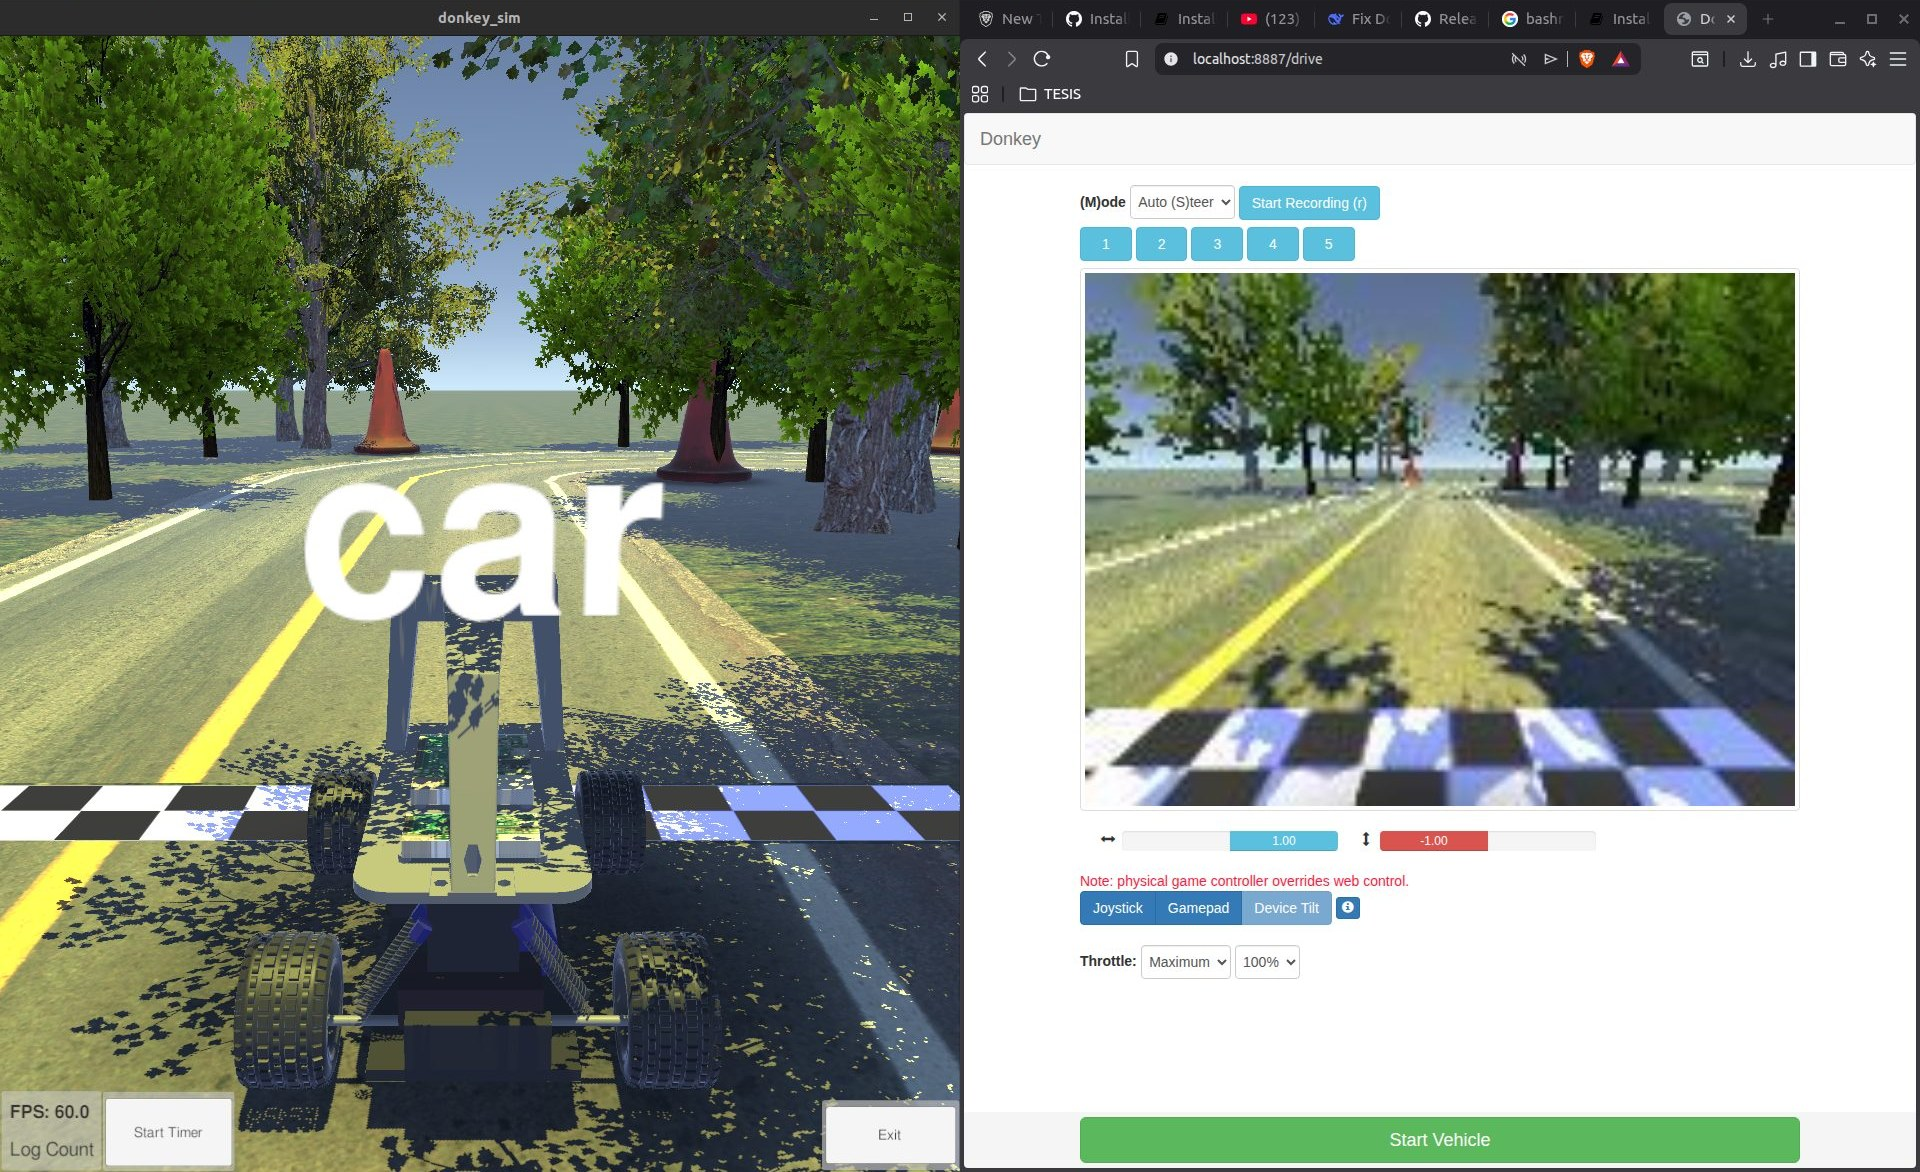
\includegraphics[height=5.2cm]{imagenes/etapa_donkeycar_simulador.jpg}\hfill
  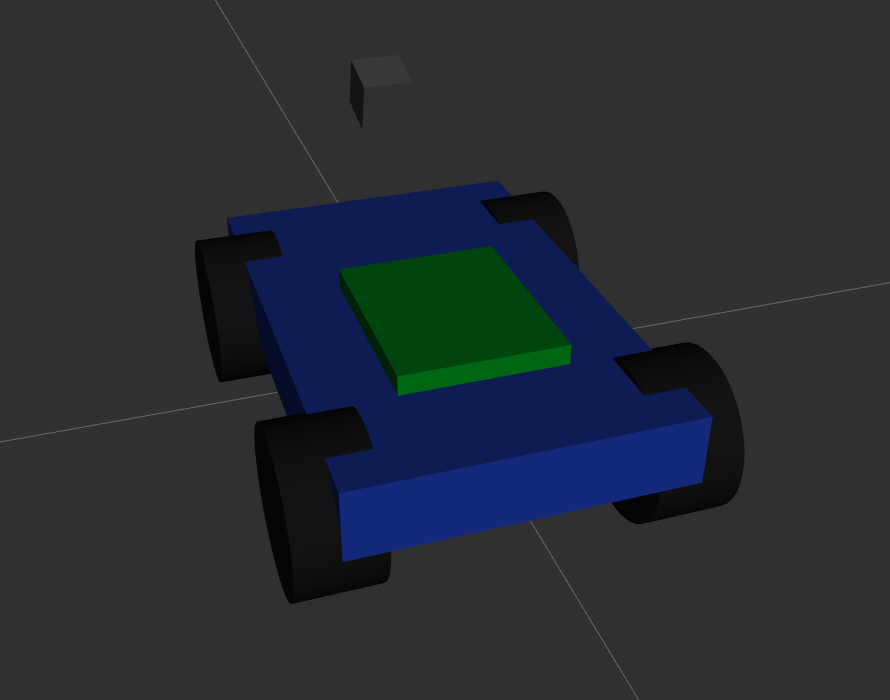
\includegraphics[height=5.2cm]{imagenes/etapa_donkeycar_modelo.png}
  \caption{Exploración de la plataforma DonkeyCar. A la izquierda, su simulador
    conducido desde la interfaz web de la plataforma, con la imagen de la cámara a bordo. A la derecha, el modelo propio del agente en el visualizador
    de ROS~2, con el chasis, las ruedas y la dirección.}
  \label{fig:donkeycar}
\end{figure}

Ese trabajo mostró tres limitaciones. El ecosistema DonkeyCar no se actualiza
desde hace años y no es compatible con las versiones recientes de ROS~2. Su
simulador no se comunica con ROS~2, así que no permite probar el mapeo, la
localización, la planificación ni la comunicación entre agentes, que son el núcleo
del proyecto. Y no existía un modelo del DonkeyCar para Gazebo con dirección
Ackermann que funcionara en ROS~2 Humble.

Para el simulador se fijaron cuatro criterios: compatibilidad con ROS~2 Humble,
vehículos con dirección Ackermann, entornos interiores y soporte para mapeo y
navegación. Entre CoppeliaSim, que proponía el anteproyecto, el simulador del
curso F1TENTH \autocite{okelly2019f1tenth} y Gazebo \autocite{koenig2004gazebo},
se eligió Gazebo por su integración directa con ROS~2 y con su sistema de control
de articulaciones. También se conservó un chasis con dirección tipo automóvil. Cada agente atiende un piso y la persona cambia de nivel por la escalera, así que ningún agente tiene que entrar a un ascensor ni subir escalones. La vuelta dentro del pasillo puede quedar a cargo de un planificador para
automóviles.

\subsection{El modelo de AWS DeepRacer y su migración a ROS~2 Humble}
\label{sec:migracion}

Una semana después se cambió al modelo del AWS DeepRacer, la decisión que hizo viable el proyecto en el tiempo disponible. Es la misma
clase de plataforma que el DonkeyCar, con chasis a escala 1:18, dirección
Ackermann, computador a bordo y software abierto. AWS publicó en código abierto su
modelo de simulación, con un complemento de cinemática Ackermann para Gazebo y
los nodos que traducen las órdenes de velocidad a los servos
\autocite{awsdeepracer2021}, y la universidad ya tenía dos. Lo que pide
el segundo objetivo, que es cinemática tipo automóvil, bajo costo y código
modificable, se cumple igual con las dos plataformas, y usar las que existían dejó
el tiempo para la coordinación. El costo fue convivir con el software del
fabricante, cuyos nodos ocupan el láser, se ejecutan con el usuario
administrador y publican sin espacio de nombres.

El software de AWS estaba escrito para ROS~2 Foxy sobre Ubuntu 20.04, y el
proyecto trabaja con Humble sobre Ubuntu 22.04. La migración necesitó tres
cambios, todos en el sistema de control de articulaciones: la orden que activa
los controladores pasó de \texttt{start} a \texttt{active}, y el componente que
publica el estado de las articulaciones cambió de nombre y de tipo. En un mundo
vacío (figura~\ref{fig:deepracer-sim}, izquierda), el modelo apareció con el láser y la cámara publicando a 62 cuadros por segundo, con un factor de tiempo
real de 1,00 y los siete controladores activos. La odometría registró 0,40~m/s
ante una orden de 0,5~m/s.

\begin{figure}[htbp]
  \centering
  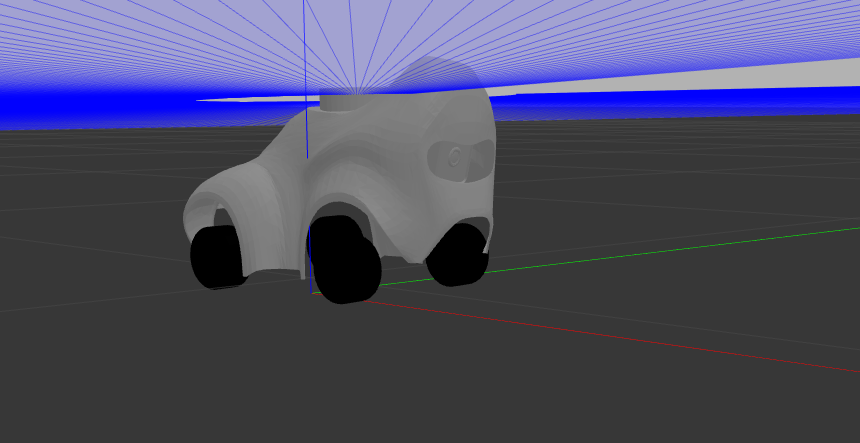
\includegraphics[height=4.6cm]{imagenes/etapa_deepracer_gazebo.png}\hfill
  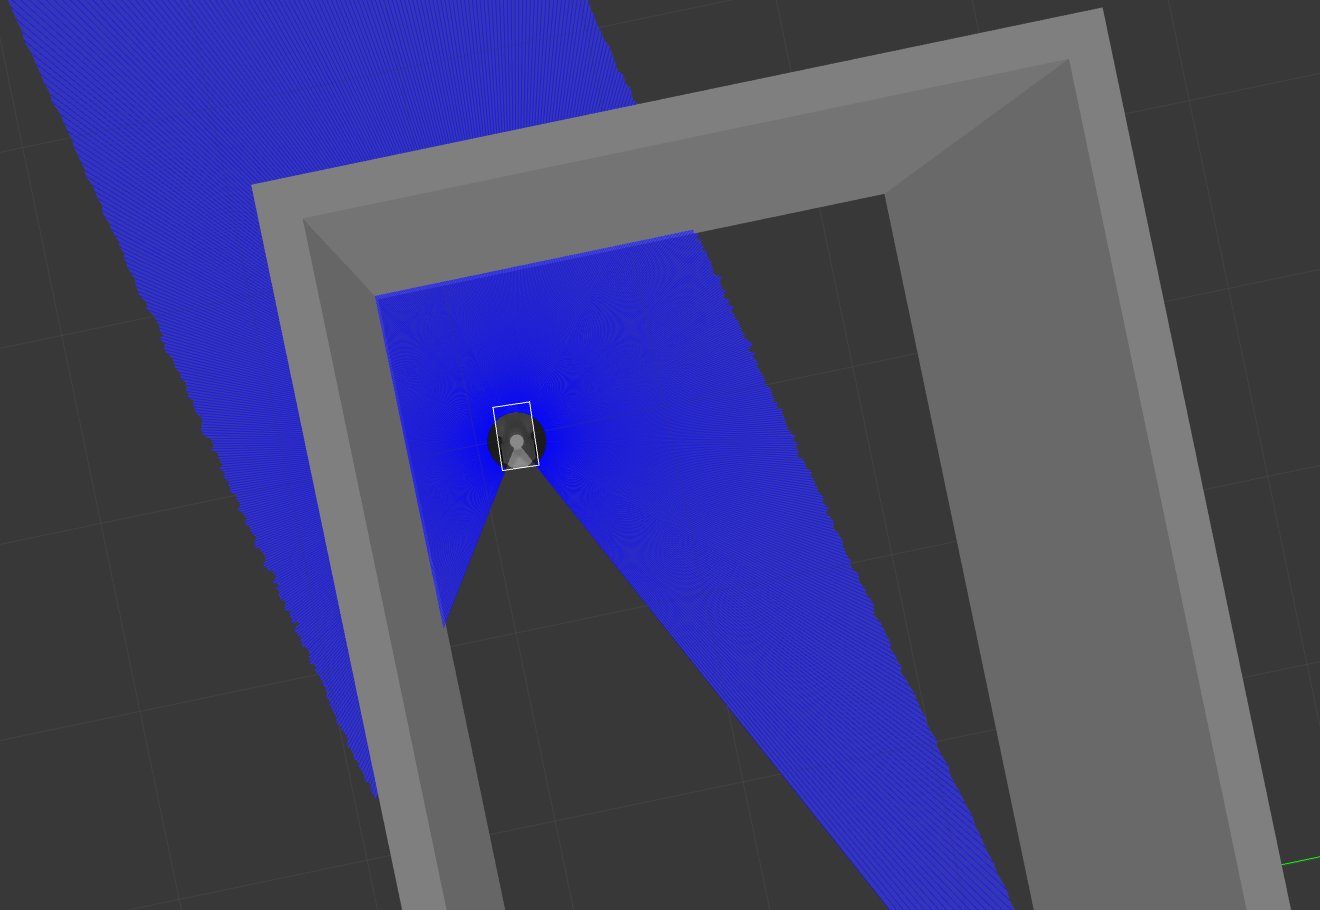
\includegraphics[height=4.6cm]{imagenes/etapa_pasillo_usta.png}
  \caption{El modelo del DeepRacer migrado a ROS~2 Humble. A la izquierda, en un
    mundo vacío, con el barrido del láser en azul. A la derecha, dentro del primer
    modelo del pasillo de la universidad, de 7 por 3~m; el sector sin barrido
    detrás del agente es el que no cubría el láser del modelo simulado.}
  \label{fig:deepracer-sim}
\end{figure}

\subsection{Los primeros entornos simulados y el seguidor de paredes}
\label{sec:primeros-entornos}

En mayo se modeló un tramo del pasillo de la universidad, de 7 por 3~m
(figura~\ref{fig:deepracer-sim}, derecha). Sobre él se programó un seguidor de paredes, como ejercicio de integración entre el láser y la cinemática del agente. La primera versión aplicaba control
proporcional-derivativo sobre un rayo lateral del láser, y saturaba el giro
porque no conocía la orientación del agente respecto a la pared. La segunda usó
la técnica de dos rayos del curso F1TENTH, que estima ese ángulo y la distancia a
la pared un metro más adelante.

En el pasillo de 7 por 3~m ninguna sintonía estabilizó al agente: el giro se
saturaba y el agente trazaba círculos o chocaba, porque su radio de giro deja
muy poco margen en 3~m de ancho. En un pasillo ampliado de 15 por 5~m convergió
por tramos, a 0,76~m de la pared frente a un objetivo de 0,5~m, y se perdía
en los extremos. La conclusión fue que un comportamiento reactivo no anticipa las restricciones de un vehículo tipo automóvil en un pasillo estrecho.
Por eso el proyecto pasó a navegar con un mapa y con un planificador que conoce
esas restricciones.

Después se modeló el primer entorno de pruebas, el piso 2 del edificio Gregorio de la universidad, donde están los salones ETM: un pasillo de 44,25~m de largo y 5,09~m de ancho. En él se comprobaron el láser, la cámara, la odometría y el árbol de transformaciones. Con ese mundo se construyó el primer mapa por localización y
mapeo simultáneos (SLAM), que se aceptó sin medirlo. Medido en septiembre,
resultó de 23,04 por 15,72~m, la mitad del largo y el triple del ancho del
pasillo. Fue la primera manifestación, sin diagnóstico entonces, de la falta de información de avance en un pasillo recto, que acabó determinando cómo se hicieron los mapas.

\subsection{La integración en simulación}
\label{sec:recorrido-sim}

El segundo semestre empezó con un cronograma replanificado, con un criterio de cierre por semana. Lo primero fue ordenar la base.
El espacio de trabajo donde se compilaba el código era una copia del repositorio
del fabricante y no un enlace al del proyecto, así que los ajustes del mapeo del
primer semestre nunca se habían ejecutado. Se enlazó al repositorio del proyecto
y se fijó el contrato de interfaces.

En agosto se aislaron los dos agentes, se construyó el entorno de dos pisos, con los pisos 2 y 3 del edificio Gregorio, y se escribieron los requisitos y el protocolo. A finales de agosto se completó la primera misión con relevo, y la campaña de treinta misiones corrió el 4 y el 5 de septiembre.

También se corrigió el modelo del agente, que tomaba la velocidad angular de la
orden estándar de ROS~2 como el ángulo del volante. Ahora el ángulo se calcula con
el modelo de bicicleta, a partir de las velocidades angular y lineal y de la
distancia entre ejes, y el error de seguimiento de las trayectorias bajó a la
mitad. La misma corrección se aplicó al nodo que mueve al agente físico.

\subsection{Del primer agente físico a la campaña con los dos}
\label{sec:recorrido-fisico}

Con los agentes físicos se trabajó en paralelo desde agosto. Se instaló el software de
la comunidad del DeepRacer \autocite{deepracercustomcar} en una Raspberry Pi~4 y
en la tarjeta original, y los agentes quedaron con su tarjeta original, con
Ubuntu 24.04 y ROS~2 Jazzy. Como la integración de
Gazebo~11 con ROS~2 no está publicada para Jazzy, desde entonces el proyecto
trabaja con dos distribuciones.

Las pruebas con los agentes físicos empezaron en los pasillos del edificio Gregorio, los mismos que se habían modelado para la simulación. Llevar allí los agentes resultó difícil por el tránsito de personas durante las pruebas, y en esos pasillos uniformes la odometría del láser no registraba el avance. Además, el modelo del piso 3 de Gregorio no correspondía a la planta real. El 2 de octubre el trabajo pasó a los pisos 3 y 4 del edificio Calatayud, que el equipo levantó con flexómetro ese mismo día. De esas medidas salieron los mapas, los mundos simulados y el catálogo de destinos de la campaña física.

En el camino hubo otros dos tropiezos: una supuesta avería que resultó ser un problema de permisos, y la saturación de la tarjeta con dos cadenas de navegación. El 21 de septiembre se decidió intentar la demostración física con seis pruebas de verificación, y la campaña con los agentes físicos corrió el 16 de octubre.

% =====================================================================
\section{Arquitectura funcional del sistema}
\label{sec:oe1}

La figura~\ref{fig:arquitectura} muestra el sistema tal como se implementó en
simulación: la interfaz por la que entra la solicitud, el coordinador que la
reparte, los dos agentes con su pila de navegación y la escalera donde ocurre el
relevo.

\begin{figure}[htbp]
  \centering
  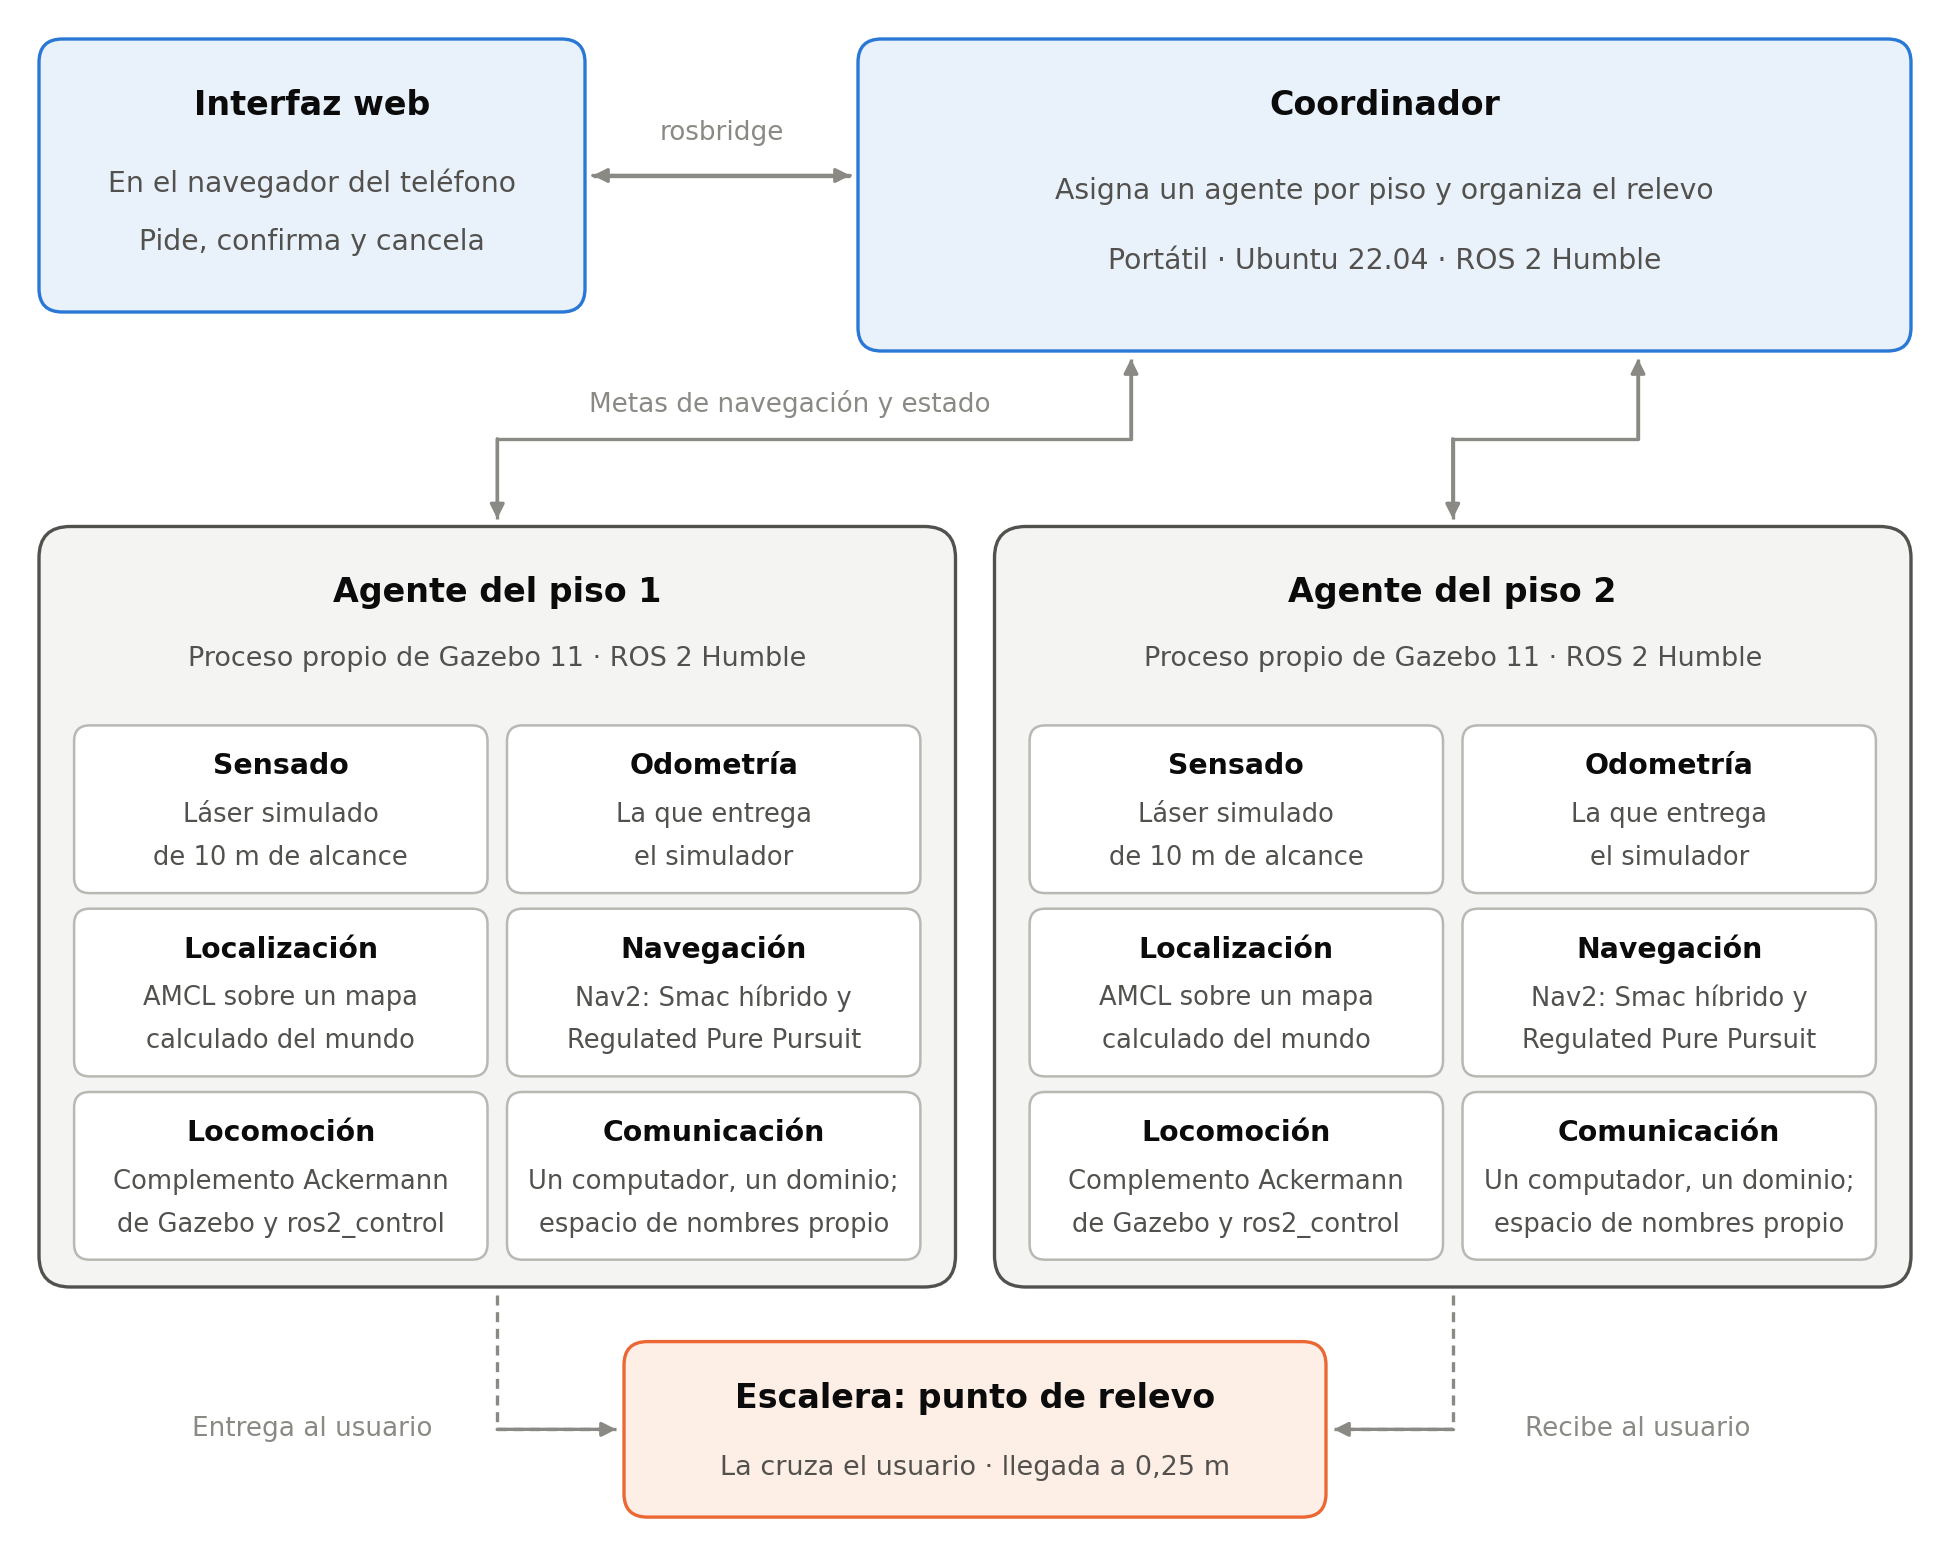
\includegraphics[width=0.86\textwidth]{imagenes/arquitectura_simulacion.png}
  \caption{Arquitectura del sistema en simulación, con un proceso de Gazebo por
    piso. Ningún agente atraviesa la zona de transición: lo que la cruza es el
    usuario, y lo que se traspasa entre agentes es la responsabilidad de guiarlo.}
  \label{fig:arquitectura}
\end{figure}

\subsection{Requisitos}

El anteproyecto no enumeró los requisitos del sistema, aunque su metodología
pedía verificar la implementación contra ellos. Se reconstruyeron al iniciar la integración a partir de los objetivos específicos, el alcance y el contrato de
interfaces. Cada requisito cita su fuente y tiene una prueba que lo declara
cumplido o no, y un requisito sin prueba no entra en la matriz.

La matriz tiene treinta y seis requisitos: veintinueve describen funciones del
sistema y siete son restricciones del alcance, como operar en interiores y en
condiciones controladas o correr la simulación en tiempo real. Al primer objetivo
le corresponden diez, sobre arquitectura, coordinación y relevo; al segundo,
seis, sobre la plataforma; al tercero, seis, sobre la interfaz; y al cuarto, siete,
sobre las métricas, el registro de cada misión y las dos campañas. La confirmación de cambio de piso y la cancelación no estaban en el anteproyecto: se añadieron al ver el sistema en uso. El avance de cada objetivo es el
promedio del estado de sus requisitos.

\subsection{El contrato de interfaces}
\label{sec:contrato}

Antes de escribir código se fijó un contrato: qué habla con qué y en qué formato.
Un coordinador central decide y manda, dos agentes, uno por nivel, ejecutan, y una
interfaz web es la vía por la que el usuario pide el servicio. La comunicación
sigue tres reglas:

\begin{enumerate}[leftmargin=*]
  \item El coordinador manda a un agente solo mediante la acción de navegación
    de ROS~2; no publica velocidades directamente. En la versión final puede
    pedirle además una media vuelta, que el agente ejecuta por su cuenta antes de navegar.
  \item La interfaz habla solo con el coordinador, nunca con los agentes.
  \item El texto que ve el usuario lo redacta el coordinador, y la interfaz lo
    muestra literal.
\end{enumerate}

La tercera regla es la que más protege el diseño: si la página interpretara el estado para decidir qué mostrar, habría dos copias de la misma lógica, y con el tiempo acabarían contradiciéndose.

El contrato se implementó como un paquete propio de mensajes de ROS~2. La acción
de guiado recibe el origen y el destino, devuelve el estado durante la misión y,
al final, el tiempo total y el número de relevos o el motivo del fallo. Cada
cambio de etapa (tabla~\ref{tab:etapas-mision}) se publica, y esas publicaciones
son las marcas de tiempo con que se calculan las métricas. La tabla~\ref{tab:contrato} reúne las interfaces entre los componentes, y la figura~\ref{fig:nodos} muestra todos los nodos del sistema en la campaña con los agentes físicos y lo que circula entre ellos.

\begin{table}[!htbp]
  \centering\footnotesize
  \caption{Interfaces del contrato entre la interfaz web, el coordinador y los agentes. \texttt{N} es el número del agente: 1 en el piso inferior y 2 en el superior.}
  \label{tab:contrato}
  \begin{tabular}{@{}p{0.36\textwidth}p{0.16\textwidth}p{0.13\textwidth}p{0.27\textwidth}@{}}
    \toprule
    \textbf{Interfaz} & \textbf{Tipo} & \textbf{Sentido} & \textbf{Contenido} \\ \midrule
    \texttt{/coordinacion/guiar\_usuario} & acción propia & interfaz $\rightarrow$ coordinador & Origen y destino; devuelve el estado durante la misión y, al final, el éxito, el tiempo total, los relevos o el motivo del fallo \\ \addlinespace
    \texttt{/coordinacion/estado\_mision} & tópico propio, 1~Hz & coordinador $\rightarrow$ interfaz & Etapa, agente activo, destino del tramo, distancia restante y texto para el usuario \\ \addlinespace
    \texttt{/coordinacion/puntos\_interes} & tópico propio, persistente & coordinador $\rightarrow$ interfaz & Catálogo de puntos de interés, con su piso \\ \addlinespace
    \texttt{/coordinacion/confirmacion\_piso} & tópico de texto & interfaz $\rightarrow$ coordinador & Confirmación de que el usuario ya cambió de piso \\ \addlinespace
    \texttt{/robotN/navigate\_to\_pose} & acción de Nav2 & coordinador $\rightarrow$ agente & Meta de cada tramo; es la única orden de movimiento \\ \addlinespace
    \texttt{/robotN/media\_vuelta} & servicio & coordinador $\rightarrow$ agente & Media vuelta antes de una meta que queda detrás \\ \addlinespace
    \texttt{/robotN/estado} & tópico propio, 2~Hz & agente $\rightarrow$ coordinador & Piso, pose en el mapa y estado del agente \\ \addlinespace
    \texttt{/robotN/odom} & odometría & agente $\rightarrow$ coordinador & Desplazamiento, con el que se marca el primer movimiento \\ \bottomrule
  \end{tabular}
\end{table}

\begin{figure}[!htbp]
  \centering
  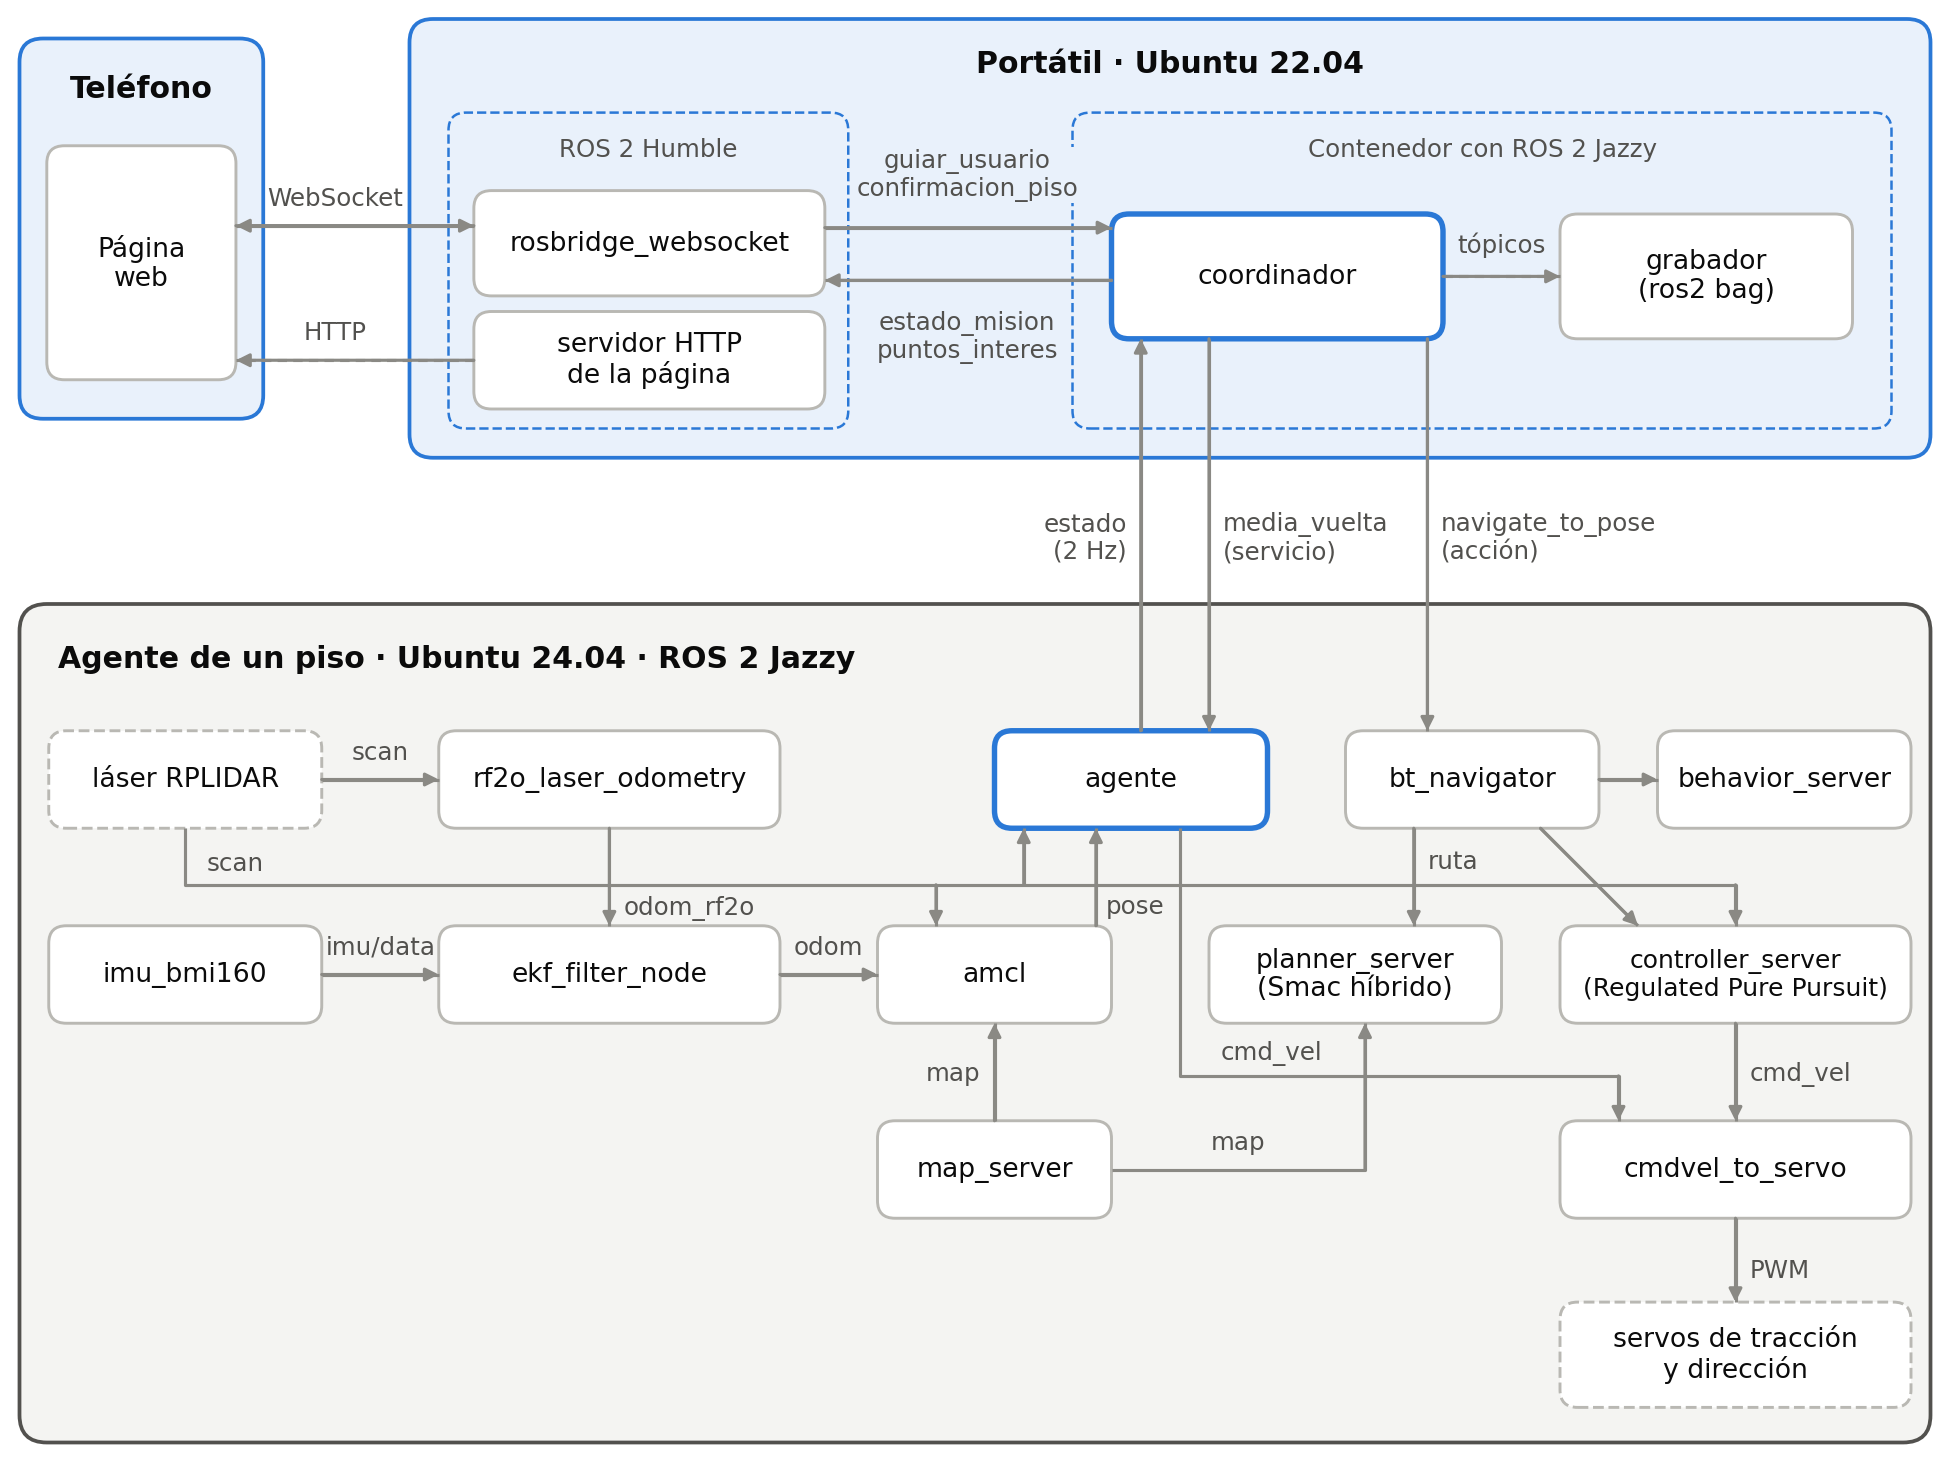
\includegraphics[width=0.96\textwidth]{imagenes/nodos_sistema.png}
  \caption{Nodos de ROS~2 del sistema en la campaña con los agentes físicos. Los dos agentes son iguales; en borde discontinuo, los componentes del fabricante. Las flechas siguen el sentido de los datos y llevan el nombre del tópico, servicio o acción. El navegador pide la ruta al planificador y su seguimiento al controlador, y la pose que estima \texttt{amcl} llega a los demás nodos por las transformadas.}
  \label{fig:nodos}
\end{figure}

\begin{table}[htbp]
  \centering\small
  \caption{Etapas de una misión, tal como las publica el coordinador.}
  \label{tab:etapas-mision}
  \begin{tabular}{@{}p{0.27\textwidth}p{0.65\textwidth}@{}}
    \toprule
    \textbf{Etapa} & \textbf{Significado} \\ \midrule
    Recibida & El coordinador aceptó la solicitud y todavía no asignó agente \\
    Primer tramo & El agente del nivel de origen va a recoger al usuario y lo guía \\
    Transferencia & El agente del otro nivel va a su punto de transferencia \\
    Esperando confirmación & El sistema espera que el usuario confirme que ya cambió de piso \\
    Segundo tramo & El agente del nivel de destino guía al usuario hasta el final \\
    Completada & La misión terminó con la llegada verificada \\
    Fallida & La misión terminó sin cumplirse, con el motivo en el texto \\
    Cancelando & El usuario canceló y el agente activo regresa a su punto de transferencia \\
    Inactiva & No hay misión en curso \\ \bottomrule
  \end{tabular}
\end{table}

\subsection{El planificador, escrito sin ROS}
\label{sec:planificador}

El relevo es el aporte declarado del proyecto, y por eso su planificación se escribió como una función pura, sin dependencia de ROS~2 ni estado propio (figura~\ref{fig:planificador}). Entran el catálogo de puntos y un par origen-destino, y salen los tramos que hay que ejecutar. Si el origen y el destino están en el mismo nivel, la misión
tiene dos tramos del mismo agente: ir a recoger al usuario y llevarlo al destino.
Si están en niveles distintos, tiene cuatro: los dos anteriores, terminando en el
punto de transferencia del nivel de origen; el desplazamiento del segundo agente
a su punto de transferencia; y el guiado final. El punto de encuentro no se negocia: es el punto de transferencia declarado de cada nivel en el catálogo.

\begin{figure}[!htbp]
  \centering
  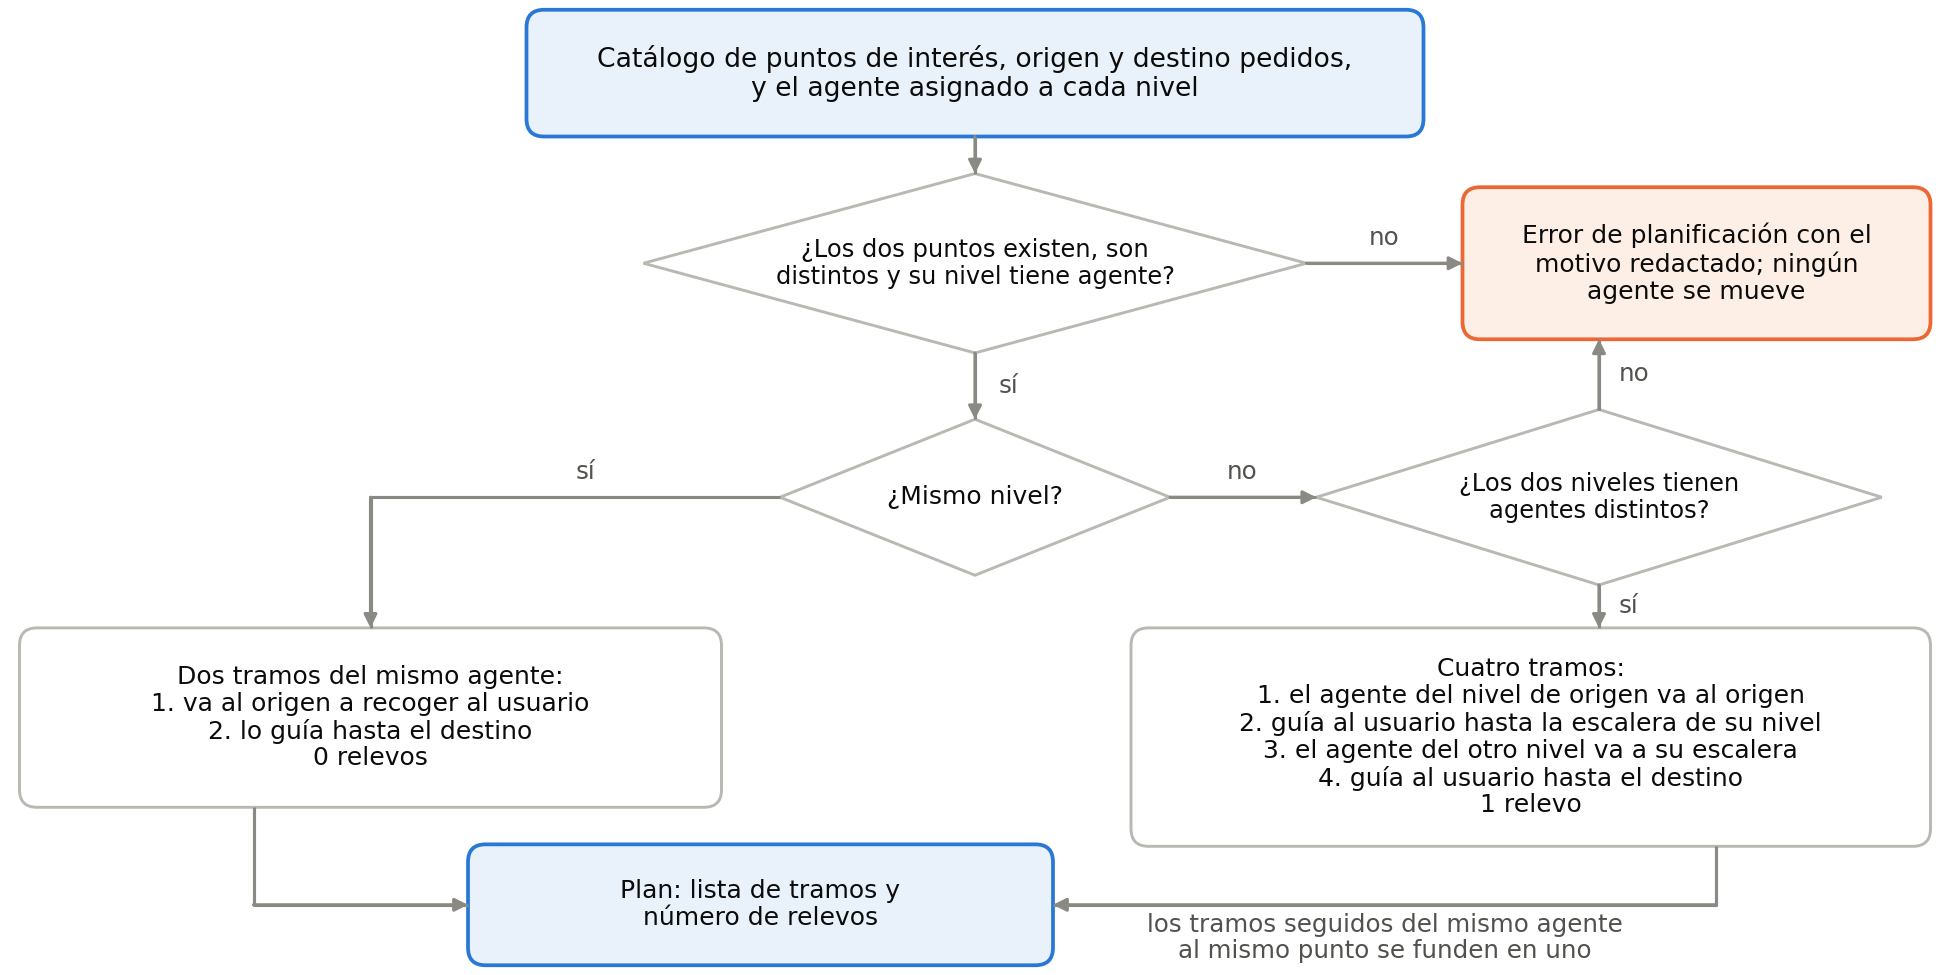
\includegraphics[width=0.84\textwidth]{imagenes/planificador.png}
  \caption{Función que planifica una misión. No usa ROS~2: recibe el catálogo, el origen, el destino y la asignación de un agente por nivel, y devuelve la lista de tramos o un error con su motivo, antes de que ningún agente se mueva.}
  \label{fig:planificador}
\end{figure}

Fue una de las decisiones más rentables del proyecto. Con el
relevo dentro del nodo, mezclado con los clientes de acción, la única forma de
comprobarlo habría sido levantar dos simuladores y observar si el agente llega.
Como función pura, una prueba automática la recorre entera en milisegundos y sin simulador. El catálogo de la simulación tiene 31 puntos de interés, y cada par ordenado de dos puntos distintos es una solicitud posible: $31 \times 30 = 930$ combinaciones de origen y destino. La prueba planifica las 930 y comprueba en todas que el plan empieza en el origen y termina en el destino, y que ningún agente recibe una meta fuera de su nivel. Comprueba también que una misión de un solo nivel usa un agente y ningún relevo, y que una de dos niveles usa los dos agentes y un relevo. Esa prueba encontró un defecto que
una corrida no habría delatado: cuando el origen o el destino era el propio punto
de transferencia de su nivel, el plan mandaba al mismo agente dos veces a la misma
pose. Nav2 devuelve éxito al instante ante un desplazamiento de cero metros, así
que en simulación no se habría visto.

\subsection{La asignación de tareas}
\label{sec:asignacion}

Cada nivel tiene un agente asignado, y esa correspondencia es un dato de
configuración, no una constante del código. El coordinador elige el agente al
aceptar la solicitud, según el nivel del origen y del destino. Con un solo agente
admisible por nivel no hace falta un optimizador, porque el método húngaro devolvería la misma tabla.

El planificador exige un único punto de transferencia por nivel y falla con un
mensaje explícito si encuentra dos. Hoy cada planta tiene una escalera y eso se
cumple; la verificación está para que, el día que haya dos, la decisión se tome a
la vista. En los agentes físicos, además, el coordinador no da por buena la llegada que
informa Nav2, sino que la comprueba con la pose que publica el agente.

\subsection{Escenarios de operación en simulación}
\label{sec:simulacion}

Los escenarios de varios pisos se construyeron primero en Gazebo~11 con ROS~2
Humble. La integración de Gazebo con ROS~2 en Humble aplica a todos los
complementos el espacio de nombres del primer modelo cargado. Por eso no fue posible tener dos agentes en un mismo proceso, y cada uno tiene su propio
simulador. El catálogo llegó a 31 puntos de interés: quince en el piso 2 y dieciséis en el piso 3 del edificio Gregorio.

Al principio los dos pisos estaban en un mismo mundo, y el láser simulado, de
10~m de alcance, veía paredes del otro piso en 61 de 1701 posiciones muestreadas. Esas posiciones estaban justo donde arranca el primer agente y donde está su punto de transferencia. Por
eso cada piso es ahora un mundo distinto, con su propio proceso de simulación. Los
dos agentes comparten un dominio de comunicaciones, separados por espacio de nombres, y la figura~\ref{fig:sim-relevo}
muestra una misión con relevo entre los dos procesos.

\begin{figure}[htbp]
  \centering
  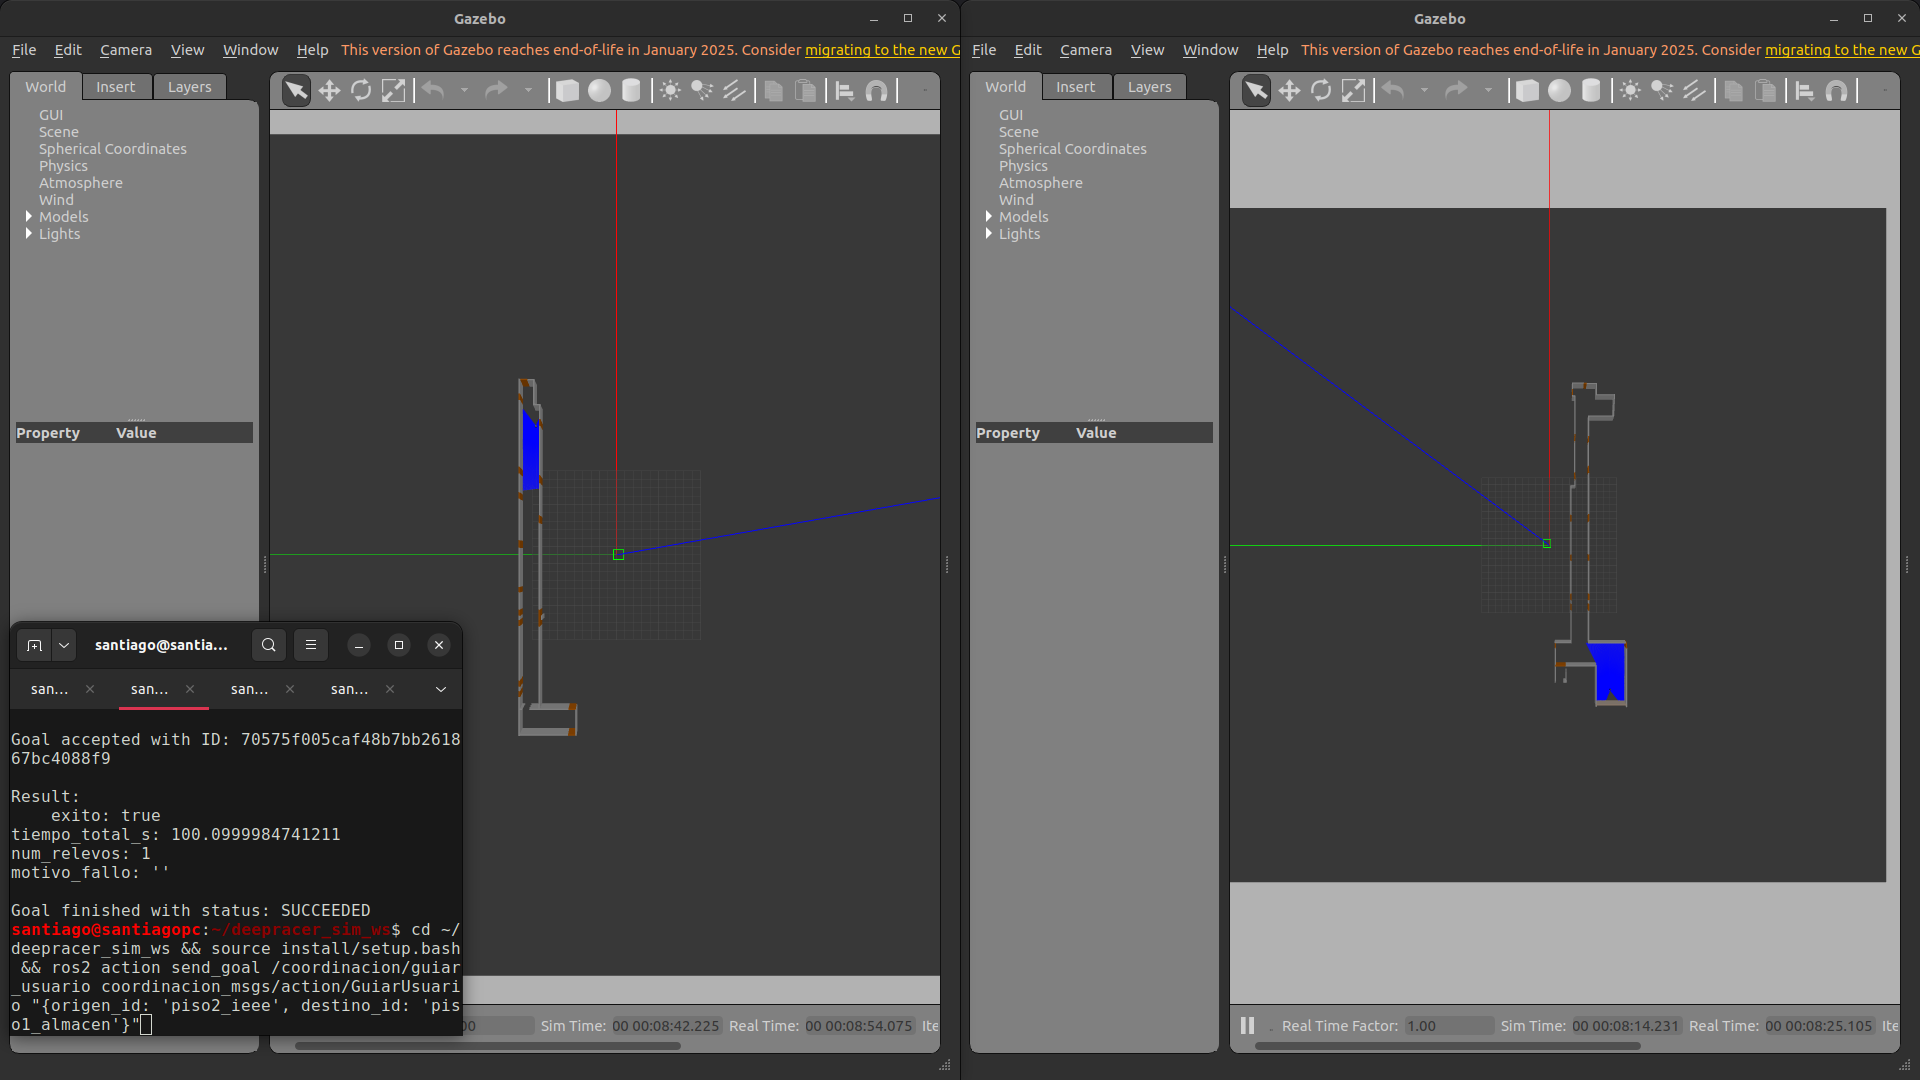
\includegraphics[width=\textwidth]{imagenes/simulacion_relevo_dos_procesos.png}
  \caption{Misión con relevo en simulación. Cada ventana es un proceso de Gazebo
    con un piso y su agente; el láser de cada uno se ve en azul. La terminal
    muestra el resultado de la acción: éxito, un relevo y 100,1~s de duración.}
  \label{fig:sim-relevo}
\end{figure}

El mapa de navegación tampoco salió de SLAM. El que se había construido cubría el
35,5~\% del largo del pasillo, medía 15,0~m de ancho frente a 5,3~m reales, y 2688
de sus 3618 celdas ocupadas, el 74~\%, no tenían ninguna pared detrás. Se reemplazó por un mapa calculado de la geometría del modelo, exacto en
simulación; como un mapa de ocupación es un corte horizontal, el del piso
superior resultó idéntico. Por último, la simulación debe correr a tiempo real
para que las métricas temporales valgan, y en las treinta misiones de la campaña
el factor de tiempo real tuvo un mínimo de 0,9917 y una media de 0,9973.

\subsection{De la simulación a los agentes físicos}
\label{sec:sim-a-vehiculos}

Al llevar el sistema a los agentes físicos se mantuvo su estructura: un coordinador, un
agente por piso, el relevo en la escalera y las reglas del contrato. También se mantuvo el código. El del coordinador,
el del planificador, el de los mensajes y el de la página es el mismo en los dos
destinos: compila sin cambios en las dos distribuciones de ROS~2 y completó una
misión en cada uno. Lo que cambió fue la implementación de los bloques. La
tabla~\ref{tab:sim-vehiculos} reúne cada cambio con su causa, y la
figura~\ref{fig:arquitectura-vehiculos} muestra el sistema como funcionó en la campaña con los agentes físicos.

\begin{table}[htbp]
  \centering\footnotesize
  \caption{Cambios en la implementación al pasar de la simulación a los agentes físicos.}
  \label{tab:sim-vehiculos}
  \begin{tabular}{@{}p{0.13\textwidth}p{0.21\textwidth}p{0.27\textwidth}p{0.31\textwidth}@{}}
    \toprule
    \textbf{Parte} & \textbf{En simulación} & \textbf{En los agentes físicos} & \textbf{Causa} \\ \midrule
    Distribución de ROS~2 & Humble en todos los componentes & Jazzy en los agentes y en el coordinador, que corre en un contenedor del portátil; Humble en la página y en rosbridge & El software de la tarjeta original solo existe para Ubuntu 24.04 con Jazzy, la simulación no existe en Jazzy, y la acción de navegación de Jazzy no es compatible con la de Humble \\ \addlinespace
    Coordinador & En el portátil, junto a los dos simuladores & En el portátil, después de un intento en uno de los agentes & Con el coordinador y el grabador en una tarjeta y las dos navegaciones encendidas, la carga subió de 6 a entre 17 y 33 y Nav2 no arrancaba \\ \addlinespace
    Comunicación & Un solo computador y un dominio de comunicaciones; un espacio de nombres por agente & Red inalámbrica con un punto de acceso de 5~GHz por piso; una partición por agente y topología en estrella hacia el portátil & Los tópicos del fabricante no llevan espacio de nombres, y los procesos de las dos cadenas, anunciándose por la red, saturaban las tarjetas \\ \addlinespace
    Locomoción & Complemento Ackermann de Gazebo con \texttt{ros2\_control} & Puente de la orden de velocidad a los servos, con una escala por agente & La tracción real tiene banda muerta y funciona en lazo abierto \\ \addlinespace
    Sensado & Láser simulado de 10~m de alcance & RPLIDAR A1M8 y la unidad inercial de la tarjeta; cámaras apagadas & Las cámaras no se usan y cargaban la tarjeta \\ \addlinespace
    Odometría & La del simulador & La del láser, combinada con la unidad inercial mediante un filtro & El agente no tiene codificadores en las ruedas, y con el láser solo el rumbo derivaba 5,9$^\circ$ por minuto \\ \addlinespace
    Mapa & Calculado de la geometría del mundo simulado & Derivado de la planta medida con flexómetro & El mapeo con SLAM a bordo no dio un mapa utilizable en ningún pasillo \\ \addlinespace
    Escenario & Pisos 2 y 3 del edificio Gregorio & Pisos 3 y 4 del edificio Calatayud, levantados con flexómetro & En Gregorio el tránsito de personas dificultaba las pruebas, el modelo no correspondía a la planta real y en sus pasillos uniformes la odometría del láser no veía el avance \\ \addlinespace
    Llegada & Tolerancia de 0,25~m & Tolerancia de 0,5~m, verificada con la pose del agente 1,5~s después de que Nav2 da la meta por alcanzada & Por la banda muerta, el agente no alcanza la precisión de la simulación, y sigue rodando cuando Nav2 declara la llegada \\ \addlinespace
    Media vuelta & La planifica Nav2, con marcha atrás & Maniobra propia del agente, vigilada con el láser y el mapa & En la salida del piso 4, de 2,5~m de ancho, la media vuelta de Nav2 abortó contra la pared \\ \bottomrule
  \end{tabular}
\end{table}

\begin{figure}[htbp]
  \centering
  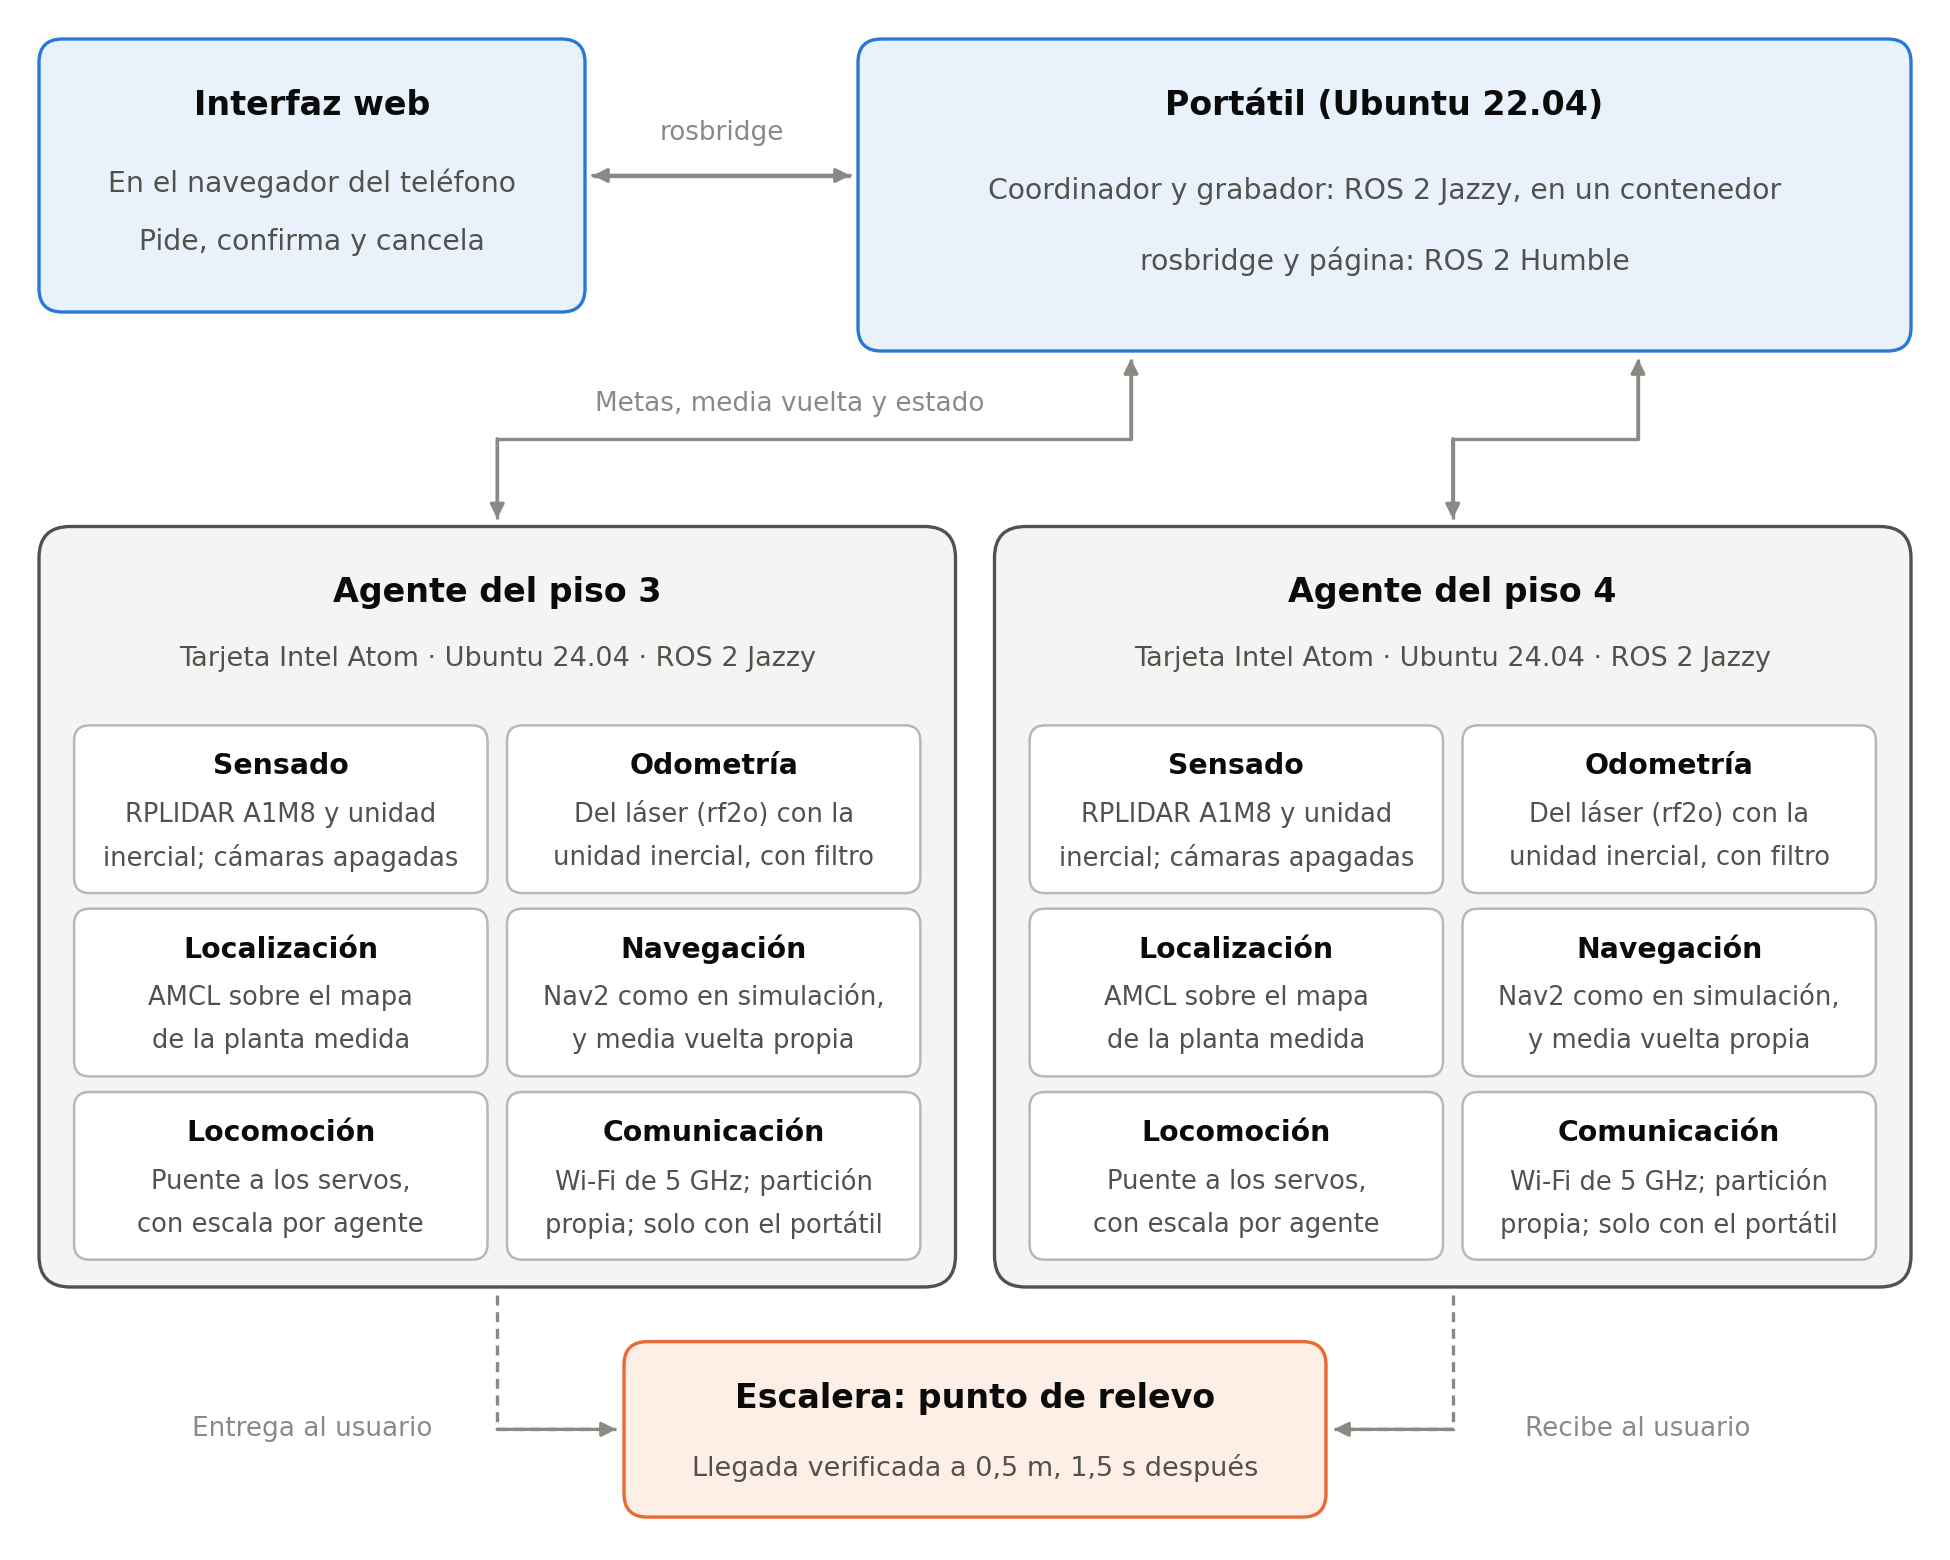
\includegraphics[width=0.86\textwidth]{imagenes/arquitectura_vehiculos.png}
  \caption{Arquitectura del sistema en la campaña con los agentes físicos, en los
    pisos 3 y 4. La estructura es la de la figura~\ref{fig:arquitectura}; cambia
    la implementación de los bloques.}
  \label{fig:arquitectura-vehiculos}
\end{figure}

% =====================================================================
\section{Plataforma robótica}
\label{sec:plataforma}

\subsection{Componentes del agente}
\label{sec:componentes}

Los dos agentes operan con su tarjeta original, para la que el software de la
comunidad solo se publica sobre Ubuntu 24.04 con ROS~2 Jazzy. La
tabla~\ref{tab:vehiculo} reúne los componentes. Cada agente atiende un piso del edificio Calatayud, uno el 3 y otro el 4. El láser que traía el kit no era el que describía el primer
informe de hardware; se identificó leyendo el modelo que reporta el propio
sensor.

\begin{table}[htbp]
  \centering\small
  \caption{Componentes de cada agente y del computador central.}
  \label{tab:vehiculo}
  \begin{tabular}{@{}p{0.25\textwidth}p{0.68\textwidth}@{}}
    \toprule
    \textbf{Componente} & \textbf{Descripción} \\ \midrule
    Chasis & AWS DeepRacer, escala 1:18, dirección Ackermann, motor de tracción con variador y servomotor de dirección \\ \addlinespace
    Cómputo & Tarjeta original, procesador Intel Atom E3930 de dos núcleos, 4~GB de memoria; Ubuntu 24.04 y ROS~2 Jazzy \\ \addlinespace
    Láser & RPLIDAR A1M8-R5: 360$^\circ$, 360 muestras por barrido, alcance de 0,15 a 12~m, entre 6,8 y 7~Hz \\ \addlinespace
    Unidad inercial & Bosch BMI160 integrada en la tarjeta, por I2C: giroscopio y acelerómetro \\ \addlinespace
    Cámaras & Estéreo; desactivadas por software, porque el sistema no las usa y cargaban la tarjeta \\ \addlinespace
    Alimentación & Una batería para el cómputo y otra de polímero de litio para la tracción \\ \addlinespace
    Computador central & Portátil con Ubuntu 22.04 y ROS~2 Humble (AMD Ryzen 5 PRO 5650U, 16~GB); el coordinador corre en un contenedor con Jazzy \\ \bottomrule
  \end{tabular}
\end{table}

\subsection{Nav2 sobre un agente que no gira sobre su eje}
\label{sec:nav2-ackermann}

La configuración por omisión de Nav2 asume tracción diferencial y propone
trayectorias que un vehículo tipo automóvil no puede ejecutar. Por eso se sustituyeron dos de sus tres capas. La
planificación global pasó al planificador híbrido A* de Smac con modelo
Reeds-Shepp, y el seguimiento, al controlador Regulated Pure Pursuit, los
dos con marcha atrás, y con una velocidad deseada de 0,5~m/s. Del árbol de
comportamiento se quitó la recuperación que gira sobre el propio eje, con la que
el agente, ante un bloqueo, movía las ruedas sin avanzar hasta agotar los
reintentos. Los parámetros tienen una variante por distribución, y una prueba
automática falla si se separan en algo distinto de las diferencias documentadas.

La cadena se puso en marcha con la escalera de siete pasos de la guía oficial de
Nav2 \autocite{nav2setup}. El orden va de las transformaciones entre marcos de referencia al
planificador y el controlador, pasando por la odometría, el láser, el mapa, la
localización y los mapas de costos. Seguir ese orden permitió aislar el problema de la odometría, porque una odometría que no mide y un planificador que no
planifica se manifiestan igual: el agente no llega. El orden importa también al
arrancar, porque los mapas de costos leen el mapa al configurarse. Por eso el
programa de arranque de los agentes activa primero el servidor de mapas y
espera a que los seis nodos de la cadena estén activos. En el laboratorio, la
cadena quedó lista en 4~min 4~s en un agente y en 4~min 22~s en el otro.

\subsection{La odometría del láser como limitación principal}
\label{sec:odometria-laser}

El agente no tiene codificadores en las ruedas, y su única odometría sale de
comparar barridos sucesivos del láser. Desde que se midió por primera vez, el 26 de agosto en simulación, hasta el cambio de edificio, el 2 de octubre, no dio una medida utilizable, por falta de información en la señal: en un pasillo recto y uniforme, cada barrido es casi idéntico al anterior y el estimador devuelve un avance cercano a cero. En los pasillos del edificio Gregorio la odometría registró desde el 1,3~\% del avance real, en simulación, hasta el 73~\%, con un agente físico en el hall del piso 3, y la localización llegaba a separarse más de dos metros de la
posición medida con flexómetro (figura~\ref{fig:hall}).

\begin{figure}[htbp]
  \centering
  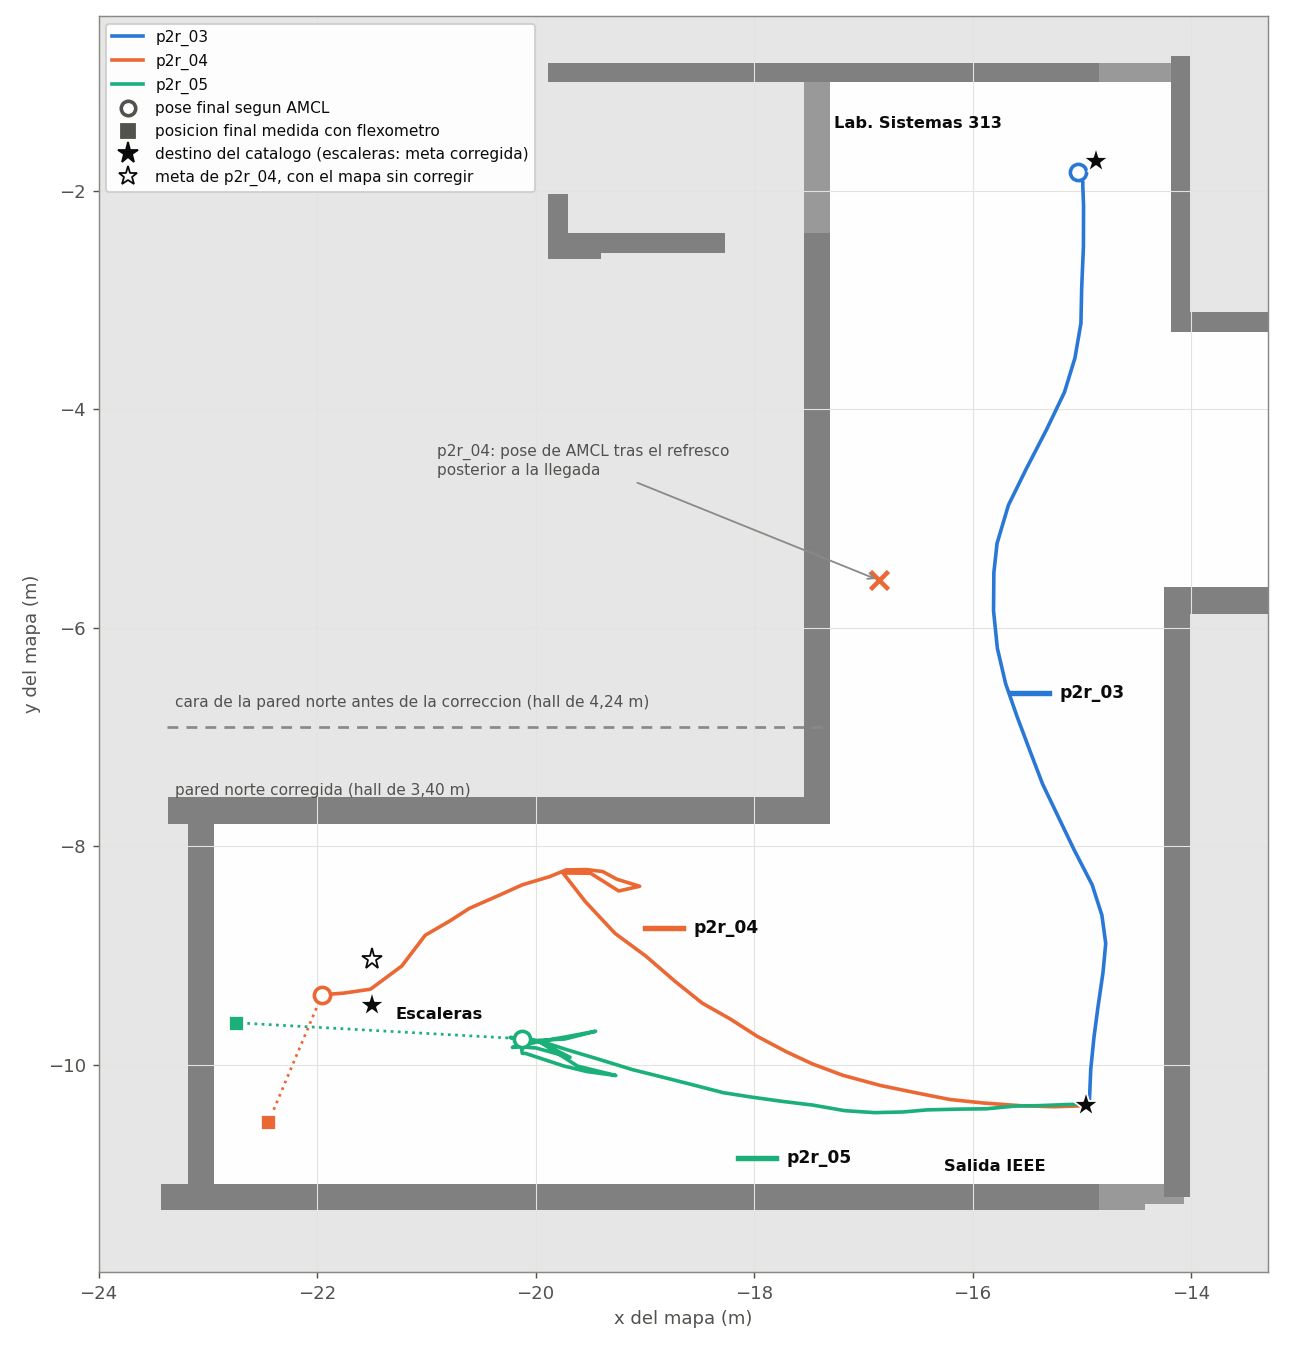
\includegraphics[width=0.6\textwidth]{imagenes/recorridos_hall_piso2.png}
  \caption{Tres recorridos de un agente en el hall del piso 3 del edificio Gregorio. El círculo es la pose que
    reporta la localización al terminar; el cuadrado, la posición real medida con
    flexómetro. La separación entre los dos es el error, y su causa está en la
    odometría, no en el algoritmo de localización.}
  \label{fig:hall}
\end{figure}

Ningún ajuste del algoritmo recupera información que la señal no contiene, y por
eso la solución fue cambiar de entorno. El criterio salió de la misma medida:
hace falta estructura no uniforme dentro del alcance del sensor durante todo el
recorrido. Los pisos 3 y 4 del edificio Calatayud la tienen. Entre las hornacinas de los salones, los
casilleros, la papelera, el ascensor y la escalera suman ocho cambios de perfil en
25~m, uno cada tres metros. Con la misma odometría y sin cambiar un parámetro, el error cayó por debajo del 5~\% (tabla~\ref{tab:odometria}). El cambio de edificio fue la decisión que hizo posible la demostración física, porque en los pasillos de Gregorio ningún ajuste habría dado al agente la información que le faltaba.

\subsection{Los mapas, derivados de medidas y no de SLAM}
\label{sec:mapas}

Los intentos de construir el mapa con SLAM en los propios agentes, en septiembre, no dieron un mapa utilizable en ningún pasillo, por la misma falta de información de avance. La vía que
funcionó fue levantar la planta con flexómetro y derivar de ese levantamiento
tanto el mundo simulado como el mapa de navegación. Así, simulación y edificio
coinciden porque salen de la misma fuente. Esa correspondencia se había dado por
supuesta, y al verificarla por primera vez resultó falsa. El modelo del edificio Gregorio daba el hall del piso 3 0,84~m más ancho de lo que es, 4,24~m frente a 3,40~m, un 25~\% de error. En los pisos 3 y 4 de Calatayud se invirtió el orden: primero se midió y después se modeló.

La herramienta que genera las plantas suma las dos paredes de cada pasillo y
avisa si no cierran dentro del 2~\%. Esa comprobación encontró cinco errores antes
de generar nada, y las dos plantas cierran al 0,32~\% y al 0,62~\%. La
figura~\ref{fig:mapa4} es el mapa del piso 4, con sus cinco puntos de interés:
tres salones, el ascensor y la escalera, que es su punto de transferencia.

\begin{figure}[htbp]
  \centering
  \includegraphics[width=\textwidth]{imagenes/mapa_piso4.png}
  \caption{Mapa de navegación del piso 4, derivado del levantamiento con
    flexómetro. El pasillo corre 25~m del extremo norte al sur; los salones
    quedan al este, y el ascensor y la escalera al oeste.}
  \label{fig:mapa4}
\end{figure}

\subsection{La banda muerta de tracción}
\label{sec:banda-muerta}

Al integrar la cadena de tracción apareció una característica de la plataforma
que condiciona la llegada: el agente no se mueve con velocidades pedidas por
debajo de 0,40~m/s. El puente que traduce la orden al variador las convertía en
tracción nula, sin ningún aviso, y el agente se detenía al entrar en la fase
final del recorrido, intentando moverse a una velocidad que su propia cadena
anulaba. Se subió a 0,40~m/s la velocidad mínima de aproximación del controlador,
y después se modificó el puente para que envíe las órdenes menores con el escalón
de tracción más bajo.

El resultado es que el agente se aproxima a la meta a 0,40~m/s y no tiene
régimen de aproximación fina. Es un límite de la plataforma, que no se corrige
afinando el controlador. Como la tracción funciona en lazo abierto, la relación
entre la orden y la velocidad real tampoco es igual en los dos agentes. Por eso el puente tiene una escala por agente, ajustada en campo: 0,85 en el del piso 3 y
0,9 en el del piso 4. Con la escala 1,0, el del piso 4 iba a 1,36~m/s y se pasaba
de la meta; con 0,9 va a 0,74~m/s.

Ante ese límite, la tolerancia de llegada con los agentes físicos se fijó en 0,5~m antes de las pruebas de navegación, mientras la simulación conserva 0,25~m.

\subsection{La unidad de medición inercial de la tarjeta}
\label{sec:imu}

Al principio el rumbo también salía de la odometría del láser, que en un pasillo
recto pierde los giros igual que el avance. Con el agente quieto, ese rumbo
derivó hasta 5,9$^\circ$ por minuto, y un giro de 90$^\circ$ hecho a mano se
registró como 19,1$^\circ$. La tarjeta incluye una unidad de medición inercial,
una Bosch BMI160 que el software del fabricante no usa. Leída directamente, midió
giros de 90$^\circ$ y 360$^\circ$ con un error de 0,1~\% a 1,3~\%, y quieta no se
desvió más de 0,3$^\circ$ en 60~s.

Se escribió un nodo que la lee y calibra el sesgo del giroscopio al arrancar. Un filtro de Kalman extendido toma de la
odometría del láser el avance y de la unidad inercial el giro; la unidad publica
a 25~Hz y el filtro corre a 15~Hz, para no cargar la tarjeta. En un giro de
90$^\circ$ contra una línea del piso, el filtro midió 90,17$^\circ$ en un agente
y 88,38$^\circ$ en el otro, y con el agente quieto su rumbo se movió
0,3$^\circ$ o menos por minuto. La posición no mejora, porque sigue saliendo del
láser. Con el rumbo estable se redujo de 1,0 a 0,5~m el margen en el que Nav2 da
la meta por alcanzada, y con ese margen se superó la prueba de navegación de un agente.

\subsection{Los dos agentes en la misma red}
\label{sec:dos-vehiculos}

Con los dos agentes encendidos aparecieron tres problemas que con uno solo no
existían. El primero fue de permisos. El software del fabricante se ejecuta con
el usuario administrador, y ROS~2 intercambia los datos entre procesos del mismo
equipo por memoria compartida, a la que solo ese usuario puede escribir. Los
programas lanzados con otro usuario veían los nodos del fabricante pero no podían
intercambiar mensajes con ellos, sin ningún error, y durante tres semanas eso
pareció una avería de uno de los agentes.

El segundo fue de nombres. Los tópicos del fabricante no llevan espacio de
nombres, así que una orden de movimiento llegaba a los dos agentes y la
odometría de cada uno recibía el láser del otro. Cada agente tiene ahora una
partición de comunicaciones propia, y la cadena del proyecto corre con un espacio
de nombres distinto en cada uno.

El tercero apareció en el primer intento de misión con relevo. Con las dos cadenas completas, todos sus procesos se anunciaban unos a otros por la red inalámbrica. La carga de la tarjeta de un agente pasó de 6 a entre 17 y 33, con
el procesador al 84--95~\%, y Nav2 no llegaba a arrancar. La respuesta fue la topología en estrella del diseño: los procesos de
cada agente solo se buscan dentro de él, lo que el coordinador necesita solo se
anuncia al portátil, y los agentes no se ven entre sí. El coordinador y el
grabador pasaron al portátil, en un contenedor con Jazzy, y verifican las
llegadas con la pose que cada agente publica dos veces por segundo.

Con todo el sistema en el laboratorio, las tarjetas quedaron al 54~\% y al 59~\%
de uso en reposo, y al 68~\% y al 74~\% navegando con las ruedas en el aire. El controlador de Nav2, que corre a 10~Hz, no bajó de 5,5~Hz. La red tiene un punto
de acceso de 5~GHz por piso, en la misma subred. Entre los dos agentes, el
tiempo de ida y vuelta de los mensajes tuvo una mediana de 5,99~ms y un percentil
95 de 11,12~ms, sin pérdidas, frente al límite de 100~ms que fija el requisito.

\subsection{La media vuelta en varios tiempos}
\label{sec:media-vuelta}

Como en la operación real, cada misión empieza donde terminó la anterior, y
el siguiente usuario queda a menudo detrás del agente, que en pasillos de 2,5 a
3,2~m de ancho tiene que dar la vuelta en varios tiempos. En el piso 4, a la
salida del pasillo de 2,5~m, la media vuelta de Nav2 abortó dos veces contra la
pared, porque el planificador proponía cada segundo una maniobra distinta.
Además, con la misma orden, el motor retrocedía a 1,7 veces la velocidad de avance, y se añadió
al puente una escala de 0,75 para la marcha atrás.

La media vuelta se escribió como una maniobra propia del agente, en lugar de seguir ajustando Nav2, que en ese caso trabajaba en el borde de lo que su controlador resuelve. La maniobra alterna
marcha atrás y avance con la dirección a tope y empieza hacia el costado con más
espacio. Cada tiempo se corta cuando la huella prevista del agente queda a
menos de 0,10~m de un obstáculo, visto por el láser o marcado en el mapa, donde la
escalera está cerrada porque el láser no ve su borde.

El coordinador la pide antes de una meta que queda a más de 110$^\circ$ del rumbo
del agente y a más de 1,5~m, y si no se completa en 120~s, sigue Nav2. En sus
primeras pruebas giró 160$^\circ$ y 167$^\circ$, en un solo tiempo cada vez, y en la campaña con los agentes físicos se ejecutó 24 veces.

% =====================================================================
\section{Interfaz de interacción con el usuario}
\label{sec:oe3}

\subsection{Una página web, no una aplicación}

El objetivo pide «una interfaz móvil», y se construyó una página web que se abre en el navegador del teléfono. Para el usuario que el proyecto declara, cumple el objetivo mejor que una aplicación, porque un visitante ocasional
no va a instalar nada para preguntar por un salón. La página funciona sin salida
a internet, porque la red del edificio puede no tenerla, y no usa bibliotecas ni
recursos externos. Son un archivo HTML, una hoja de estilo y dos programas en JavaScript, que sirve el propio portátil. Se comunica con
ROS~2 por el puente \textit{rosbridge}, que no tiene autenticación, así que el firewall del portátil solo admite conexiones desde la red de los agentes.

El primer programa es un cliente propio del protocolo del puente, porque la
biblioteca de cliente más difundida implementa las acciones de la primera generación de ROS. El segundo es la lógica de la página. Recibe el catálogo de puntos al conectarse y el estado de la misión una
vez por segundo, pide y cancela con la acción de guiado y publica la
confirmación de cambio de piso.

\subsection{Lo que el usuario ve}

El usuario elige el origen en una lista y el destino en un catálogo con búsqueda
por nombre, donde cada destino muestra su piso y, si queda en el otro nivel, la
marca «con relevo». Durante la misión, la página muestra un título calculado a
partir de la etapa, el texto que redacta el coordinador, el agente que está
guiando, hacia dónde va, el destino final y la distancia restante. Una franja de
cinco pasos (preparando, tramo 1, relevo, tramo 2 y fin) marca el paso actual (figura~\ref{fig:hri}, izquierda).

\begin{figure}[!htbp]
  \centering
  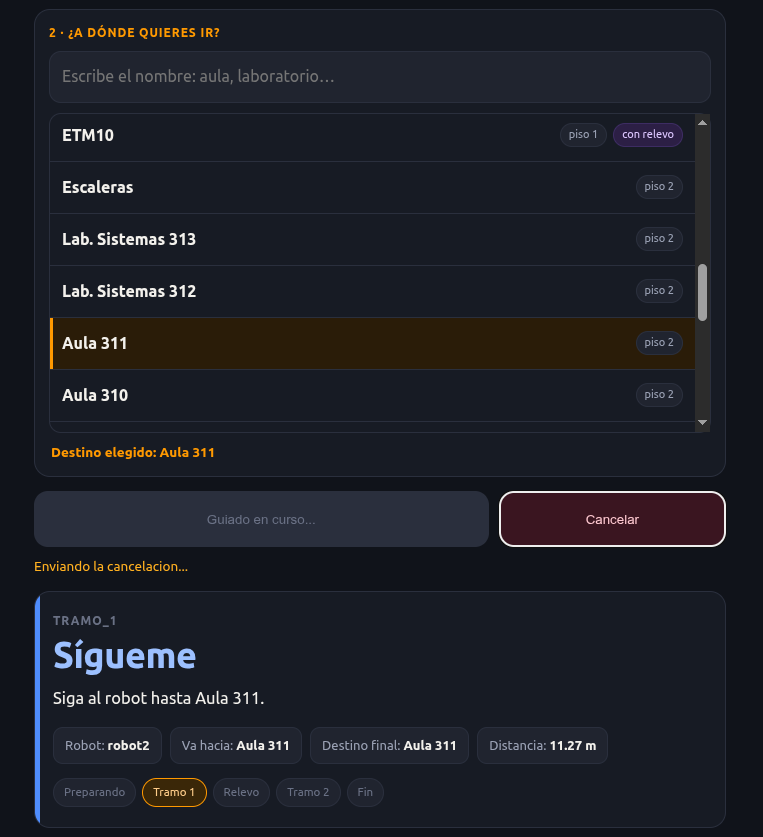
\includegraphics[height=8.4cm]{imagenes/hri_seguimiento.png}\hspace{0.04\textwidth}%
  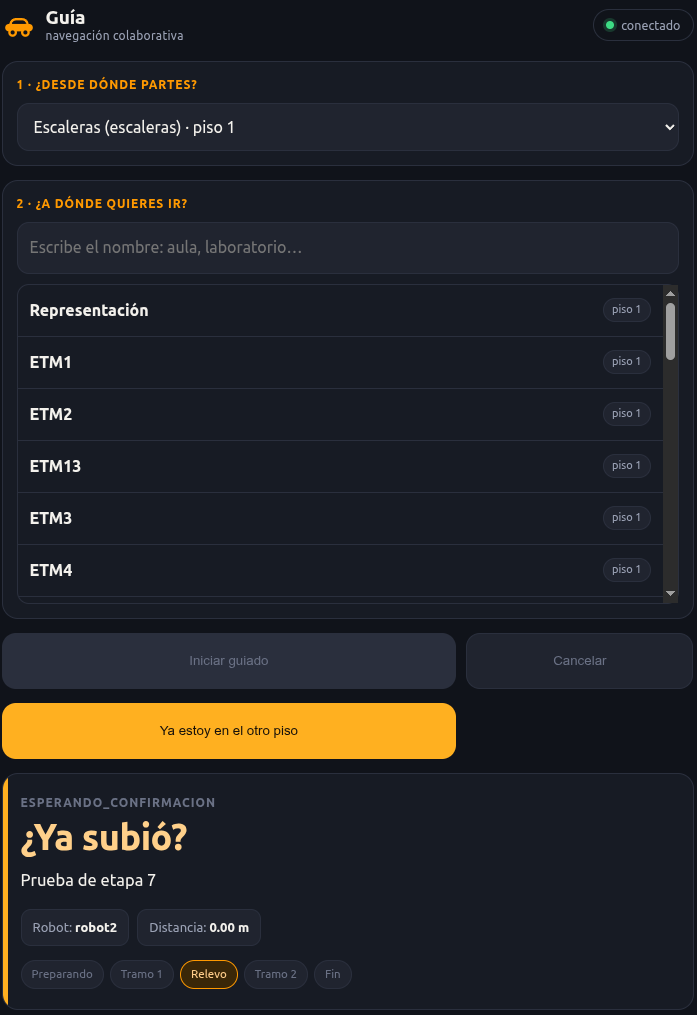
\includegraphics[height=8.4cm]{imagenes/hri_confirmacion_piso.png}
  \caption{Interfaz web. A la izquierda, durante una misión en simulación: el destino elegido, el botón de cancelar y el panel de estado del primer tramo, con el texto del coordinador, el agente activo y la distancia restante. A la derecha, en la etapa de espera de confirmación, durante su prueba automática: el estado lo publica la prueba, con el texto «Prueba de etapa 7», y la página muestra el botón «Ya estoy en el otro piso», de la versión anterior a los ajustes que siguieron a las pruebas con los agentes físicos.}
  \label{fig:hri}
\end{figure}

La interfaz se verificó contra el coordinador real: el catálogo, una misión con
sus etapas, el texto del coordinador mostrado literal y el botón que se reactiva
al terminar. También se operó una misión completa con relevo desde un teléfono
real conectado a la red de los agentes, sin tocar el computador. Las dos
funciones que siguen se añadieron después de ver el sistema en uso.

\subsection{Confirmación de cambio de piso}

En una misión entre niveles, el segundo agente llega a su escalera y espera al
usuario, pero no puede saber si la persona ya subió. Sin una pausa explícita, la
misión podía darse por completada con el usuario todavía en el piso equivocado, y
la instrumentación lo habría registrado como éxito. Por eso, cuando el segundo
agente llega a su punto de transferencia, el coordinador pasa a la etapa de espera de confirmación. La página muestra entonces un botón para confirmar el cambio de
piso, que solo existe en esa etapa (figura~\ref{fig:hri}, derecha). A los 60~s sin
confirmación aparece un aviso, y a los 120~s la misión termina como fallida. Los
plazos se cuentan desde que llega el agente, para que un agente lento no le
consuma tiempo al usuario, y se miden con el reloj del sistema y no con el de la
simulación. Si el usuario confirma antes de que el agente llegue, la
confirmación se retiene y se aplica al llegar.



Se verificó en simulación con una corrida por camino. Confirmar a los pocos segundos termina la misión con éxito, y confirmar pasados los 60~s hace aparecer el aviso en el teléfono. No confirmar deja la misión fallida a los 120~s, con el
motivo redactado.

\subsection{Cancelación}

El botón de cancelar existía pero no hacía nada, y no se había detectado. El
servidor de acción del coordinador no registraba la función que responde a la
cancelación, y ROS~2 rechaza por omisión, sin informar, toda cancelación que no
tenga esa función. Al corregirlo se añadió el comportamiento que faltaba: la
misión pasa por la etapa de cancelación, el agente activo regresa al punto de
transferencia de su piso, y la misión cierra como fallida con un texto que lo
dice. En simulación, con una corrida cancelada y una de control, el agente
quedó a 0,121~m de su punto de regreso.

Con los agentes físicos se cancelaron seis misiones, al menos una en cada etapa, y en
las seis el agente volvió a su escalera, a entre 0,07 y 0,34~m de su punto. Esas
pruebas mostraron un defecto que la simulación no podía mostrar, porque la media
vuelta propia se añadió después. Nav2 conserva durante un tiempo las metas terminadas, y mientras tenía una cancelada en su lista, el agente se declaraba en error y rechazaba la media vuelta. Sin ella, Nav2 intentaba girar
por su cuenta en el pasillo y oscilaba. Ahora la media vuelta solo espera a que no
haya una meta en curso: antes de la corrección se rechazaron ocho de quince
medias vueltas, y después ninguna de diez.

\subsection{Ajustes tras las pruebas con los agentes físicos}
\label{sec:ajustes-campo}

Las pruebas con los agentes físicos mostraron tres defectos de la página. El título de
la etapa de confirmación preguntaba siempre «¿Ya subió?», lo que al subir
resultaba brusco y al bajar del piso 4 al 3 era falso. Ahora sale de comparar el
piso de origen con el del agente que espera, como «Suba con calma al piso 4» o «Baje con calma al piso 3». El botón dice «Ya estoy en el piso 4», o el piso que
corresponda.

Ese cambio se hizo el día de la campaña, antes de correrla, y aun así los
teléfonos mostraron la versión anterior, porque el servidor no le indicaba al
navegador cuándo volver a pedir la página. Ahora la página se sirve con la
indicación de comprobarla cada vez que se abre. El tercer defecto fue de nombres:
los dos ascensores se llamaban igual en la lista y en una misión se eligió el del
piso equivocado, así que los nombres repetidos se muestran ahora con su piso, como
«Ascensor (piso 3)». Los tres ajustes se verificaron con pruebas automáticas y
después con un teléfono y los agentes físicos, en una misión de subida y otra de
bajada.

% =====================================================================
\section{Protocolo experimental e instrumentación}
\label{sec:protocolo}

El protocolo se escribió antes de instrumentar el sistema, a propósito: un protocolo redactado después
de ver los datos tiende a acomodarse a lo que salió, por ejemplo eligiendo el
umbral que deja fuera las corridas malas. El protocolo fija las métricas con su
definición operativa, el criterio de éxito, el tamaño de muestra y una lista
cerrada de causas de descarte, y cada versión queda fechada en el historial del
repositorio.

\subsection{Definiciones operativas}

Una métrica sin un evento de inicio y uno de fin medibles por una máquina no se
puede reportar. La tabla~\ref{tab:metricas} da los dos eventos de cada una. Todas
las marcas salen de un mismo reloj: en simulación, el de la simulación; en los agentes físicos, el del computador que graba.

\begin{table}[htbp]
  \centering\small
  \caption{Definición operativa de las cuatro métricas del anteproyecto.}
  \label{tab:metricas}
  \begin{tabular}{@{}p{0.2\textwidth}p{0.36\textwidth}p{0.36\textwidth}@{}}
    \toprule
    \textbf{Métrica} & \textbf{Inicio} & \textbf{Fin} \\ \midrule
    Tiempo de respuesta & El coordinador acepta la solicitud & Primera de tres muestras seguidas de la odometría del agente asignado con velocidad de al menos 0,02~m/s \\ \addlinespace
    Tiempo de asignación & Primera publicación de la etapa recibida & Primera publicación del primer tramo, con el agente asignado \\ \addlinespace
    Tasa de éxito & \multicolumn{2}{p{0.72\textwidth}}{Proporción de misiones exitosas sobre las corridas válidas} \\ \addlinespace
    Continuidad entre niveles & El primer agente alcanza su punto de transferencia & Primer movimiento del segundo agente \\ \bottomrule
  \end{tabular}
\end{table}

Una misión es exitosa si cumple tres condiciones. La pose final del agente, en
su odometría, está a 0,25~m o menos del destino declarado en el catálogo; en los agentes físicos el umbral es de 0,5~m. La misión llegó a la etapa completada sin pasar
por fallida. Y, si era entre niveles, hubo un relevo.

La regla central del protocolo es que el éxito se mide contra
la odometría del agente, nunca contra el resultado que devuelve Nav2. Una
navegación puede terminar en éxito y haber dejado al agente lejos del destino:
en las primeras pruebas en simulación, una de tres metas devolvió éxito con el
agente a 0,296~m. Aceptar ese resultado sería dejar que el sistema se evalúe a
sí mismo.

El tiempo de asignación resultó menor que el paso de 100~ms del reloj de la
simulación, así que se reporta como una cota por misión y se caracterizó aparte,
en un banco de pruebas con el reloj del sistema. La continuidad se definió primero como una condición binaria, que resultó no poder fallar, y se reemplazó por el intervalo del relevo, una magnitud que sí varía.

\subsection{Diseño de la campaña en simulación}

La campaña en simulación tiene treinta misiones en dos grupos de quince. En las de un mismo piso, el origen y el destino están en el mismo nivel y no hay relevo; sirven de comparación. En las de dos pisos hay un relevo, y son las que responden la pregunta de investigación.

Los pares de origen y destino salen de un sorteo, porque con pares elegidos a mano se corre el riesgo de probar justo los recorridos que funcionan. Se sortean entre los puntos del catálogo menos los dos puntos de transferencia, catorce en el piso 2 y quince en el piso 3, que dan 392 pares posibles dentro de un mismo piso y 420 entre pisos, y ningún par se repite. La semilla del sorteo es la fecha en que se hace, escrita como año, mes y día, y el listado se guarda en el repositorio antes de la primera corrida. Así, nadie puede probar semillas hasta obtener un sorteo conveniente.

Las diez primeras misiones salieron de un sorteo con la semilla 20260822 en el que todas las misiones entre pisos subían del piso 2 al 3 y todas las de un solo piso se quedaban en el 2. El grupo con relevo era el único que navegaba por el piso 3, y una diferencia entre los grupos no habría podido atribuirse al relevo. Las veinte restantes se sortearon de nuevo el 4 de septiembre, con la semilla 20260904, para que cada grupo quedara repartido entre los dos pisos: en el de un mismo piso, ocho misiones en el piso 2 y siete en el 3; en el de dos pisos, ocho de subida y siete de bajada.

Una corrida fallida cuenta como fallo. Solo se descarta si la causa es ajena al sistema y está en una lista cerrada, escrita antes de la campaña, que admite la caída del simulador, un controlador del agente que no
se activa, el factor de tiempo real por debajo de 0,99, un fallo de la máquina
anfitriona o una cancelación por una causa externa anotada antes de conocer el
resultado. Si los descartes superan el 20~\% de las corridas, la campaña no es
válida.

\subsection{Instrumentación}
\label{sec:instrumentacion}

Cada misión deja una grabación de datos de ROS (\textit{rosbag}) con los tópicos
del coordinador y de los dos agentes. Un programa compone a partir de ella el
registro de la misión, en un formato estructurado que se valida contra un esquema versionado. El registro contiene las marcas de cada etapa, la trayectoria de cada agente, la pose
final, el error de llegada y su procedencia. Un segundo programa comprueba la
integridad de los registros y calcula las cuatro métricas con sus intervalos de
confianza. Se escribió antes de la campaña, y encontró dos defectos que después
habrían sido irreparables: la continuidad no tenía campo en el esquema, y el
intervalo que citaba el protocolo no se reproducía con el método declarado.

Con los agentes físicos, el grabador corre en el contenedor con Jazzy, y un programa adapta la grabación al formato que leen las
herramientas de Humble. El registro usa el reloj del computador, la tolerancia de
0,5~m y el mapa de cada piso. La llegada la verifica el coordinador con la pose que publica el agente, 1,5~s después de que Nav2 la da por alcanzada (figura~\ref{fig:instrumentacion}). Nav2 la declara en cuanto el agente entra en su margen, y el agente sigue rodando.
En las llegadas medidas en el piso 4, el agente estaba a entre 0,53 y 0,62~m de
la meta en la última orden de avance, y un segundo después, ya quieto, a entre
0,09 y 0,53~m. La distancia de llegada se guarda con su procedencia, medida con
flexómetro o tomada de la localización del agente, y el analizador advierte cuando no hay medida externa, como ocurrió en la campaña con los agentes físicos.

\begin{figure}[!htbp]
  \centering
  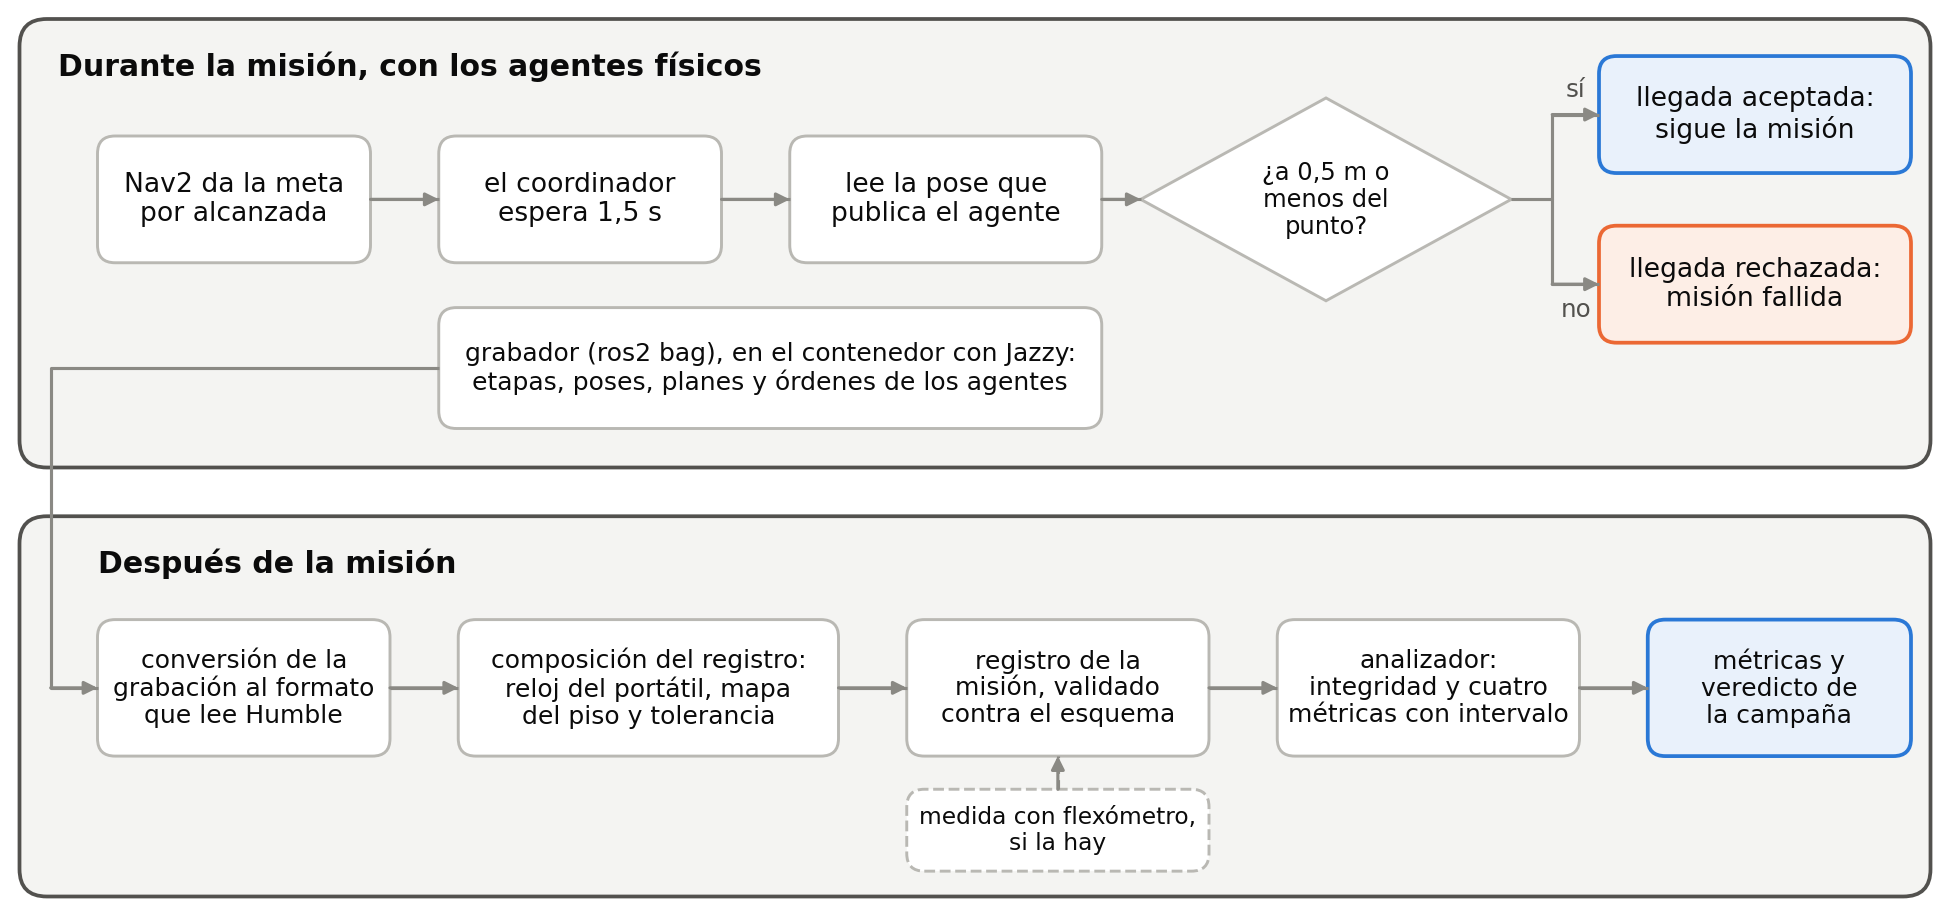
\includegraphics[width=\textwidth]{imagenes/instrumentacion.png}
  \caption{Instrumentación de una misión. Arriba, la verificación de la llegada que hace el coordinador con los agentes físicos; abajo, el camino de la grabación hasta las métricas de la campaña. En simulación el camino es el mismo, sin la conversión de formato y con la tolerancia de 0,25~m.}
  \label{fig:instrumentacion}
\end{figure}

\subsection{Pruebas de verificación de la demostración física}
\label{sec:pruebas-verificacion}

La demostración con los agentes físicos se organizó en seis pruebas de verificación
sucesivas. Cada prueba tiene un criterio escrito antes de correrla y lo que
significa no superarla (tabla~\ref{tab:pruebas-verificacion}). Se fijaron tres
fechas de revisión en octubre, y después de la última, el 16 de octubre, no se
toman más datos.

\begin{table}[htbp]
  \centering\small
  \caption{Pruebas de verificación de la demostración física y su estado al
    cerrar la toma de datos.}
  \label{tab:pruebas-verificacion}
  \begin{tabular}{@{}p{0.24\textwidth}p{0.52\textwidth}p{0.16\textwidth}@{}}
    \toprule
    \textbf{Prueba} & \textbf{Criterio} & \textbf{Estado} \\ \midrule
    Actuación & El agente responde a las órdenes de dirección y tracción & Superada \\ \addlinespace
    Odometría & Error de 10~\% o menos sobre un recorrido conocido de 5~m o más & Superada \\ \addlinespace
    Navegación de un agente & Un agente llega de un punto a otro con Nav2, con la llegada verificada & Superada \\ \addlinespace
    Dos agentes en la misma red & Los dos agentes y el coordinador coexisten sin conflicto de nombres & Superada \\ \addlinespace
    Misión con relevo & Una misión con relevo sobre los dos agentes, con su registro & Superada \\ \addlinespace
    Campaña con los agentes físicos & Entre 5 y 10 repeticiones del protocolo con su registro & Superada \\ \bottomrule
  \end{tabular}
\end{table}

Para la campaña con los agentes físicos se sortearon el 13 de octubre, con la semilla 20261013, diez misiones entre los pisos 3 y 4 del edificio Calatayud: cinco de subida y cinco de bajada. Se corrieron en ese orden y sin reubicar los agentes entre misiones, como ocurriría en la operación real.

% =====================================================================
%  RESULTADOS (versión recortada, para comparar con
%  capitulos/08-resultados.tex)
%
%  Recorte del 2026-10-25:
%   - «Ancho del intervalo de confianza» sale de las limitaciones: repetía lo
%     dicho con la tabla de la campaña en simulación.
%   - La llegada sin flexómetro se explica una sola vez, en la última
%     limitación; las condiciones de las pruebas solo remiten a ella.
%   - Voz de los autores donde se interpreta un resultado; registro
%     impersonal en lo que se reporta.
%   - Figuras y tablas con [htbp].
%  Ninguna cifra de resultado sale del capítulo.
% =====================================================================
\chapter{Resultados}
\label{cap:resultados}

Las dos campañas, en simulación y con los vehículos, se reportan por separado. La de
simulación produce la evidencia estadística, y la de los vehículos demuestra que
el sistema opera sobre la plataforma real.

% ---------------------------------------------------------------------
\section{Evaluación en simulación}
\label{sec:res-sim}

La campaña corrió treinta misiones sorteadas: quince de control, con origen y
destino en el mismo piso, y quince entre pisos, con un relevo. El analizador la
dictaminó válida, sin ningún descarte, frente a un máximo admitido del 20~\%.

\subsection{Tasa de éxito}

Una misión es exitosa si la pose final queda a 0,25~m o menos del destino,
medida contra la odometría y no contra el resultado de Nav2, y si llega a
completarse sin pasar por fallo. La tabla~\ref{tab:exito} da la tasa de cada grupo
con su intervalo de confianza de Wilson al 95~\% \autocite{wilson1927probable}.

\begin{table}[htbp]
  \caption{Tasa de éxito de la campaña en simulación, con intervalo de confianza
    de Wilson al 95~\%.}
  \label{tab:exito}
  \begin{tabular}{@{}lcccc@{}}
    \toprule
    \textbf{Misiones} & \textbf{n} & \textbf{éxitos} & \textbf{tasa} & \textbf{intervalo al 95~\%} \\ \midrule
    Campaña completa & 30 & 26 & 86,7 \% & 70,3 -- 94,7 \% \\
    Mismo piso (control) & 15 & 12 & 80,0 \% & 54,8 -- 93,0 \% \\
    Entre pisos, con relevo & 15 & 14 & 93,3 \% & 70,2 -- 98,8 \% \\ \bottomrule
  \end{tabular}
\end{table}

Lo que podemos afirmar es que la tasa de éxito supera el 70~\%, no que sea del
86,7~\%. Con treinta misiones el intervalo mide 24 puntos porcentuales de ancho, y
ese límite es de diseño: solo se reduce con más muestra. El 86,7~\% es el
estimador puntual y se reporta siempre junto a su intervalo. Los intervalos de
los dos grupos se solapan, así que la comparación entre ellos no sostiene ninguna
conclusión, aunque el estimador puntual apunte en contra de la intuición: las
misiones con relevo salieron mejor que las de control.

\subsection{Causa común de los cuatro fallos}

Las cuatro misiones fallidas quedaron a 0,295, 0,284, 0,311 y 0,347~m del
destino, frente a una tolerancia de 0,25~m. Las cuatro se quedaron cortas:
ninguna se pasó del destino ni terminó en otro sitio. Los cuatro fallos se deben
al límite de precisión de la aproximación final, y ninguno a la coordinación. El
error de llegada del conjunto tiene una mediana de 0,106~m y va de 0,019 a
0,347~m.

\subsection{Tiempo de respuesta y tiempo de asignación}

El tiempo de respuesta se reporta por escalones, y no con media y desviación, por
una razón de instrumento (tabla~\ref{tab:respuesta}).

\begin{table}[htbp]
  \caption{Tiempo de respuesta de las treinta misiones, en escalones del reloj de
    la simulación.}
  \label{tab:respuesta}
  \begin{tabular}{@{}lcccc@{}}
    \toprule
    \textbf{Tiempo de respuesta} & 0,1 s & 0,2 s & 0,3 s & 0,4 s \\ \midrule
    Misiones & 10 & 15 & 4 & 1 \\ \bottomrule
  \end{tabular}
\end{table}

Los cuatro valores son múltiplos exactos de 100~ms, el paso con que avanza el
reloj de la simulación, y la resolución del instrumento vale entre el 25~\% y el
100~\% de la magnitud medida. Una mediana de 0,2~s significa «uno o dos pasos del
reloj», no «doscientos milisegundos», y dar media y desviación sugeriría una
precisión que el reloj no entrega. Lo que sí se sostiene es la cota, que además es
lo que le importa a un usuario: el robot arranca en menos de medio segundo.

El tiempo de asignación quedó por debajo de 100~ms en las treinta misiones,
varios órdenes de magnitud por debajo de un paso del reloj. Por eso se
caracterizó aparte, en un banco de pruebas con el reloj del sistema: mediana
entre 154 y 175~\textmu s y máximo de 306~\textmu s. La
figura~\ref{fig:simulacion} muestra una misión de la campaña.

\begin{figure}[htbp]
  \centering
  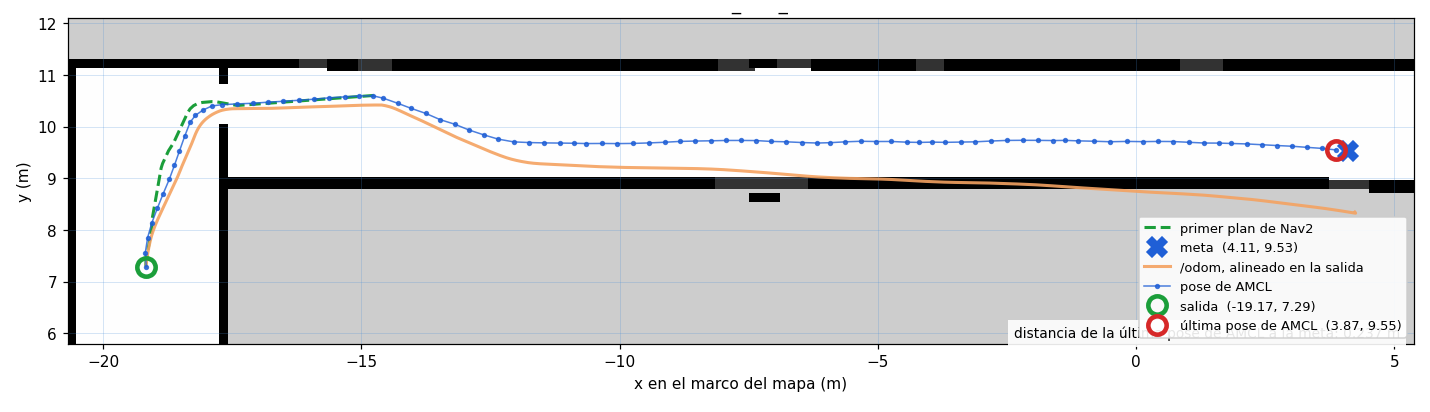
\includegraphics[width=\textwidth]{imagenes/corrida_simulacion.png}
  \caption{Una misión de la campaña en simulación. Se superponen el primer plan
    que calcula el navegador, la pose estimada a lo largo del recorrido y la
    odometría cruda. La separación creciente entre las dos últimas es la deriva
    que la localización corrige contra el mapa.}
  \label{fig:simulacion}
\end{figure}

% ---------------------------------------------------------------------
\section{Evaluación con los vehículos}
\label{sec:res-hw}

\subsection{La odometría del vehículo}

La odometría del vehículo sale de comparar barridos sucesivos del láser, y
durante meses no produjo una medida utilizable. La tabla~\ref{tab:odometria}
reúne lo que se midió en cada entorno, como fracción del avance real medido con
flexómetro.

\begin{table}[H]
  \centering\small
  \caption{Fracción del avance real que registra la odometría, por entorno. El
    criterio de la prueba es un error de 10~\% o menos.}
  \label{tab:odometria}
  \begin{tabular}{@{}lccl@{}}
    \toprule
    \textbf{Entorno} & \textbf{Recorrido} & \textbf{Registrado} & \textbf{Criterio} \\ \midrule
    Pasillo simulado, 46,9 m & largo & 37,9 \% & no cumple \\
    Pasillos de los pisos 1 y 2 & largo & 5,7 \% y 1,3 \% & no cumple \\
    Hall del piso 2 & 6 m & 73 \% & no cumple \\
    Cuarto cerrado, desplazado a mano & 3 m & 96,3 -- 101,9 \% & cumple \\
    Pasillo del piso 4 & 6,68 m & 95,4 \% & cumple \\
    Pasillo del piso 4 & 14,57 m & 103,3 \% & cumple \\
    Pasillo del piso 4, con la unidad inercial & 8,08 m & 101,9 \% & cumple \\
    Pasillo del piso 4, con la unidad inercial & 2,82 m & 104,9 \% & cumple \\ \bottomrule
  \end{tabular}
\end{table}

El estimador es el mismo en todas las filas; lo que cambió fue el entorno. En un
pasillo recto y uniforme la información de avance no está en la señal del
sensor, y ningún ajuste la recupera (sección~\ref{sec:teo-localizacion}). En un
pasillo con hornacinas, casilleros y quiebres, con ocho cambios de perfil en
25~m, la misma odometría queda dentro del $\pm$5~\% sin cambiar un parámetro. Con
las dos mediciones del pasillo del piso 4, de 6,68 y 14,57~m, el director dio por superada la prueba de odometría, de la que dependía todo lo demás
sobre los vehículos. Las dos últimas filas ya incluyen la unidad inercial
(sección~\ref{sec:imu}); el segundo de esos tramos mide 2,82~m, por debajo de los
5~m que pide el criterio, y se incluye como dato de la misma cadena.

\subsection{La navegación y la precisión de llegada}
\label{sec:res-g3}

La prueba de navegación de un vehículo pide un recorrido de punto a punto con Nav2 y la llegada verificada con flexómetro, a 0,5~m o menos del destino. Es la tolerancia que fijó el director para los vehículos reales. En la primera
sesión en el piso 4 las dos llegadas medidas quedaron a 0,57 y 0,62~m, cortas,
porque Nav2 daba entonces la meta por alcanzada a 1,0~m. Con la unidad inercial
integrada (sección~\ref{sec:imu}) ese margen bajó a 0,5~m. En la sesión siguiente, uno de los vehículos recorrió en el piso 4 tres tramos encadenados, sin
que nadie lo tocara entre uno y otro, y después regresó a la salida
(tabla~\ref{tab:g3} y figura~\ref{fig:cadena}).

\begin{table}[htbp]
  \centering\small
  \caption{Cadena de tres tramos en el piso 4 y regreso a la salida: llegada de
    cada tramo.}
  \label{tab:g3}
  \begin{tabular}{@{}llcccl@{}}
    \toprule
    \textbf{Tramo} & \textbf{Destino} & \textbf{Tiempo} & \textbf{Recuperaciones} & \textbf{A la meta} & \textbf{Medida} \\ \midrule
    1 & Salón 403 & 13,5 s & 1 & 0,26 m & estimada \\
    2 & Salón 402 & 27,8 s & 1 & 0,45 m & flexómetro \\
    3 & Salón 401 & 5,2 s & 0 & 0,06 m & flexómetro \\
    Regreso & Salida & 62,8 s & 6 & 0,34 m & flexómetro \\ \bottomrule
  \end{tabular}
\end{table}

Las llegadas medidas quedaron dentro de la tolerancia de 0,5~m, y el director dio por superada la prueba. La llegada al Salón 403 no se midió porque en ese
momento no había flexómetro, y se estimó con el error de los otros dos tramos. El
regreso a la salida incluyó una media vuelta en el tramo ancho frente a los
salones, que Nav2 resolvió con seis recuperaciones.

\begin{figure}[htbp]
  \centering
  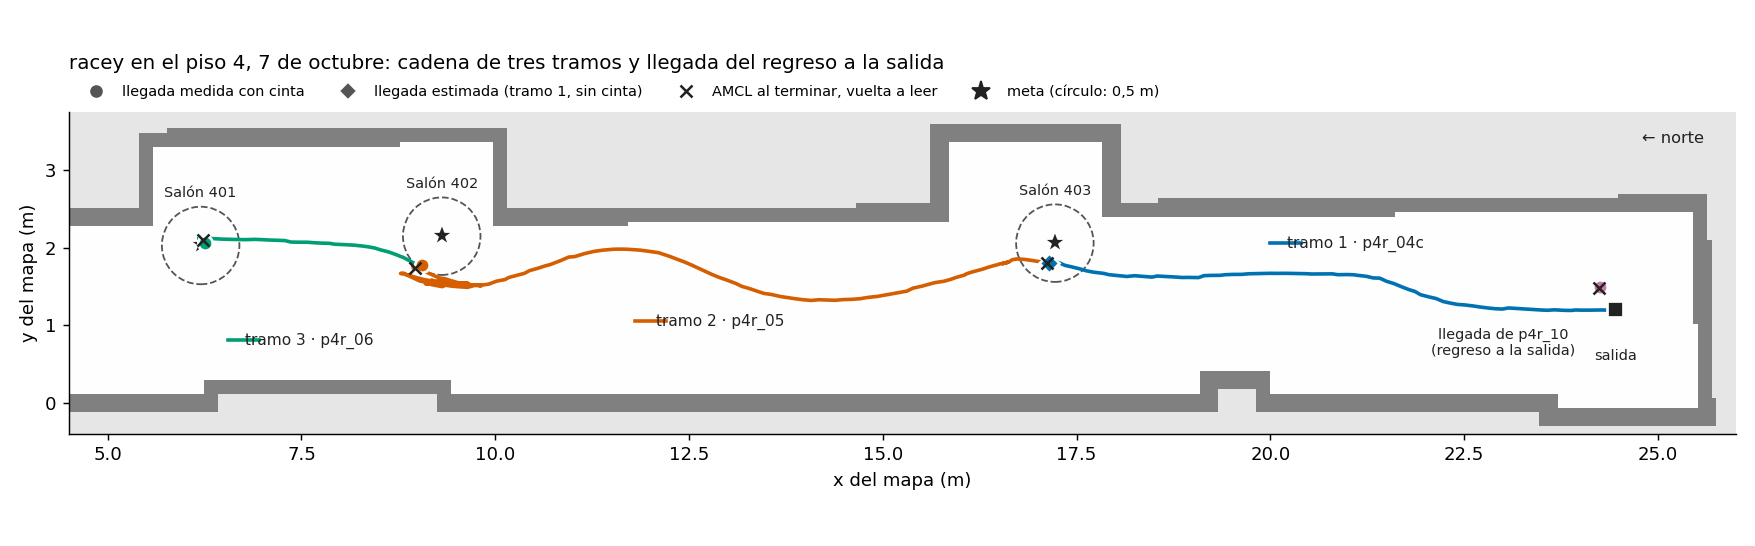
\includegraphics[width=\textwidth]{imagenes/cadena_piso4.png}
  \caption{Cadena de tres tramos en el piso 4 y regreso a la salida: recorrido
    según la localización, llegadas medidas con flexómetro, la llegada estimada
    al Salón 403 y la pose de la localización al terminar cada tramo.}
  \label{fig:cadena}
\end{figure}

Al día siguiente, el otro vehículo recorrió el piso 3 en cinco tramos
encadenados, con dos medias vueltas entre ellos, y los cinco terminaron con éxito
y sin recuperaciones. Esas llegadas no se midieron con flexómetro, y al forzar a la
localización a recalcular su pose al final de cada tramo, esta se desplazó entre 0,61 y 0,86~m. La pose que publica la localización al detenerse el vehículo va atrasada, y por eso la llegada que vale es la medida con flexómetro. Lo que condiciona la precisión de llegada sigue siendo la banda
muerta de tracción (sección~\ref{sec:banda-muerta}): el vehículo se aproxima a la
meta a 0,40~m/s y no tiene régimen de aproximación fina.

% ---------------------------------------------------------------------
\section{Evaluación del sistema completo con los dos vehículos}
\label{sec:res-completo}

El sistema completo funcionó sobre los dos vehículos. La misión con relevo del
Salón 302 al Salón 402 se completó, y de las diez misiones sorteadas para la
campaña, las nueve que llegaron a correr se completaron, todas con relevo. La
décima quedó interrumpida porque el computador portátil se apagó por falta de
batería.

\subsection{Condiciones de las pruebas}

Las pruebas se hicieron en los pisos 3 y 4, con un vehículo en cada piso. El
coordinador y el grabador corrieron en el portátil, y cada misión se pidió desde
la página web en un teléfono conectado a la red de los vehículos. Los autores
hicieron de usuario: pidieron cada misión, acompañaron a los vehículos y
confirmaron el cambio de piso en la página. Los vehículos no se reubicaron entre
misiones, y cuando el destino quedaba detrás del vehículo, el coordinador pidió la
media vuelta en varios tiempos (sección~\ref{sec:media-vuelta}). La llegada se verificó con la localización de cada vehículo y no con flexómetro (sección~\ref{sec:lim-llegada}).

\subsection{La misión con relevo}

La primera prueba del sistema completo fue una misión del Salón 302, en el piso 3,
al Salón 402, en el piso 4. Se completó en 132,5~s, con un relevo y con la llegada
a 0,444~m del destino. Entre la llegada del primer vehículo a la escalera y el
arranque del segundo pasaron 61,1~s. Fue el segundo intento: en el primero, el
coordinador rechazó la llegada del vehículo del piso 3 al Salón 302, adonde iba a
recoger al usuario, porque su localización lo situaba a 0,59~m del punto.

Esa sesión sirvió de ensayo del montaje, y en ella los autores eligieron las
misiones sin seguir el sorteo. De las doce misiones grabadas, siete se completaron
y cinco terminaron fallidas: en cuatro, el coordinador rechazó una llegada con el
vehículo a entre 0,51 y 0,78~m del punto, y en la otra Nav2 abortó la navegación.
Estas misiones no forman parte de la campaña.

\subsection{La campaña con las misiones sorteadas}

Las diez misiones de la campaña se sortearon antes de correr, con una semilla
fija, entre los puntos de interés de los dos pisos: cinco de subida y cinco de
bajada (sección~\ref{sec:pruebas-verificacion}). Corrieron en el orden del
sorteo, y la tabla~\ref{tab:campana-vehiculos} da el resultado de las nueve que
llegaron a correr.

\begin{table}[htbp]
  \centering\small
  \caption{Campaña con los dos vehículos: las nueve misiones sorteadas que
    corrieron, todas completadas con un relevo. La llegada es la de la
    localización del vehículo, con una tolerancia de 0,5~m.}
  \label{tab:campana-vehiculos}
  \begin{tabular}{@{}cllccc@{}}
    \toprule
    \textbf{N.\textsuperscript{o}} & \textbf{Origen} & \textbf{Destino} & \textbf{Tiempo total} & \textbf{Respuesta} & \textbf{Llegada} \\ \midrule
    1 & Ascensor, piso 3 & Salón 403 & 52,3 s & 0,51 s & 0,435 m \\
    2 & Salón 302 & Salón 401 & 90,1 s & 0,27 s & 0,202 m \\
    3 & Salón 401 & Salón 302 & 87,6 s & 3,90 s & 0,143 m \\
    4 & Salón 403 & Salón 303 & 78,9 s & 1,25 s & 0,420 m \\
    5 & Salón 402 & Salón 301 & 105,4 s & 0,66 s & 0,285 m \\
    6 & Salón 301 & Salón 401 & 89,8 s & 2,97 s & 0,226 m \\
    7 & Ascensor, piso 4 & Salón 301 & 81,7 s & 0,87 s & 0,234 m \\
    8 & Salón 302 & Salón 403 & 81,8 s & 0,95 s & 0,214 m \\
    9 & Salón 303 & Salón 402 & 92,6 s & 0,63 s & 0,299 m \\ \midrule
    \multicolumn{3}{@{}l}{Mediana} & 87,6 s & 0,87 s & 0,234 m \\ \bottomrule
  \end{tabular}
\end{table}

Con nueve éxitos en nueve misiones, el intervalo de Wilson al 95~\% va del 70,1 al
100~\%. Lo que podemos afirmar es que la tasa de éxito sobre los vehículos supera
el 70~\%, la misma cota que sostiene la campaña en simulación. Expresado como en
la sección~\ref{sec:teo-evaluacion}, nueve repeticiones sin fallo demuestran una
fiabilidad mínima de 0,81 con un 85~\% de confianza.

El error de llegada tuvo una mediana de 0,234~m y fue de 0,143 a 0,435~m. El
tiempo total, desde la solicitud hasta la llegada verificada, tuvo una mediana de
87,6~s y fue de 52,3 a 105,4~s. El tiempo de respuesta, desde que el coordinador
acepta la solicitud hasta que el vehículo asignado empieza a moverse, tuvo una
mediana de 0,87~s y quedó por debajo de 1,3~s en siete de las nueve misiones. Los
dos valores más altos, 3,90 y 2,97~s, son de misiones en que el vehículo ya estaba
en el punto de origen. El coordinador verificó esa llegada, que no exigía moverse,
con la espera de 1,5~s, y el primer movimiento fue la media vuelta hacia la
escalera. El tiempo de asignación fue de 0,3~ms en las nueve misiones, medido con el reloj del portátil e incluyendo el paso del mensaje hasta el grabador, del mismo orden que el del banco de pruebas
(sección~\ref{sec:res-sim}). En las nueve misiones los vehículos hicieron 24 medias
vueltas, de entre 160 y 171$^\circ$, en uno a cuatro tiempos cada una.

La figura~\ref{fig:campana-vehiculos} descompone el tiempo de cada misión en sus
etapas. Ir a recoger al usuario tomó entre 2,2 y 30,6~s, según dónde había
terminado la misión anterior. El guiado en el piso de origen tuvo una mediana de
24,2~s, y el guiado en el piso de destino, de 24,8~s.

\begin{figure}[htbp]
  \centering
  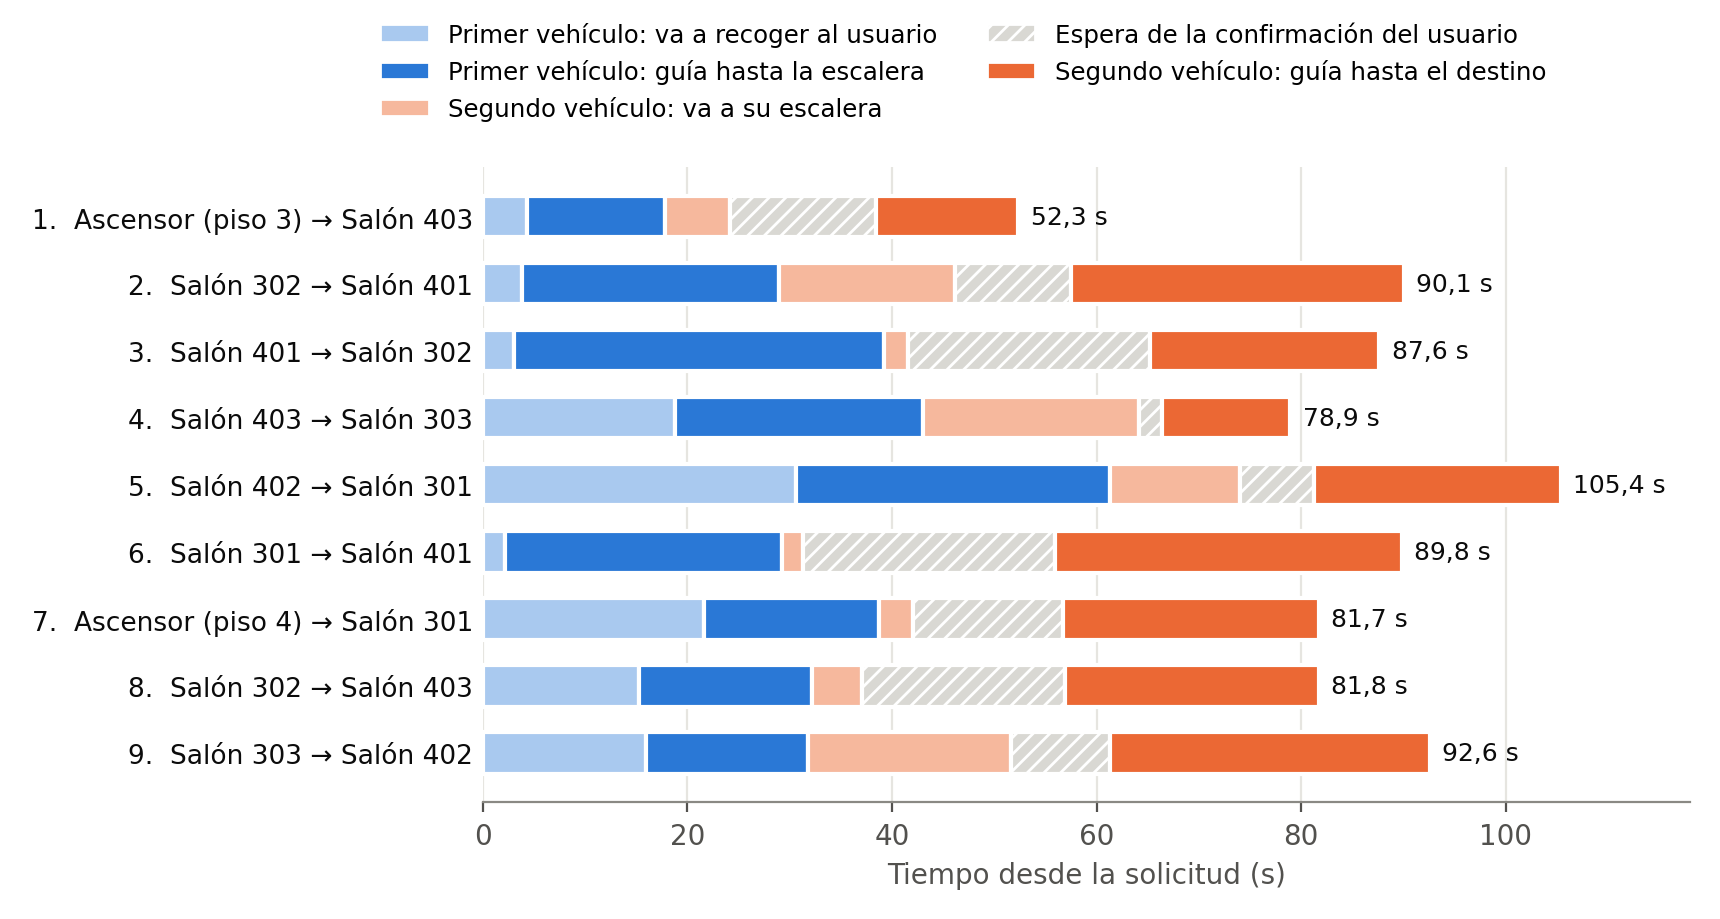
\includegraphics[width=\textwidth]{imagenes/campana_vehiculos_etapas.png}
  \caption{Duración de cada etapa en las nueve misiones de la campaña con los
    vehículos, según las marcas de etapa del coordinador. El tramo rayado es la
    espera de la confirmación de cambio de piso, contada desde que el segundo
    vehículo está en su escalera.}
  \label{fig:campana-vehiculos}
\end{figure}

\subsection{El relevo entre los dos vehículos}

En las nueve misiones el relevo se produjo y el coordinador no pasó por el estado
inactivo ni quedó sin agente asignado. Como en simulación, ese criterio no puede
fallar por la forma en que está construido (sección~\ref{sec:limitaciones}). La medida que informa es el intervalo del relevo: el tiempo desde que el primer
vehículo llega a su escalera hasta el primer movimiento del segundo.

Ese intervalo tuvo una mediana de 1,22~s, pero la cifra junta dos situaciones. En
cinco misiones el segundo vehículo tuvo que desplazarse hasta su escalera, en
cuatro desde el destino de la misión anterior y en una para corregir su posición
unos centímetros, y arrancó en menos de 1,3~s. En las otras cuatro ya estaba en la
escalera, su primer movimiento fue el del guiado final, después de la
confirmación, y el intervalo, de 12,9 a 27,5~s, mide sobre todo cuánto tardó la
persona en confirmar.

Para la persona, lo que cuenta es el tiempo entre la llegada a la escalera del
piso de origen y el arranque del guiado en el piso de destino. En ese tiempo
cambia de piso, el segundo vehículo llega a su escalera si no estaba allí, y la
persona confirma en la página. Tuvo una mediana de 24,8~s y fue de 18,0 a
29,5~s. La confirmación, desde que el segundo vehículo estaba en su escalera, tomó
entre 2,3 y 24,7~s, y el aviso de los 60~s no llegó a mostrarse en ninguna misión.

\subsection{Criterio de conteo e incidencias}

La campaña cuenta, por decisión de los autores, una corrida por misión: la que se
completó. El protocolo, en cambio, cuenta como fallo toda corrida fallida, y por
eso los intentos que no entran en la tasa se declaran aquí. Las misiones 1 y 2 se
completaron en el segundo intento. Los dos primeros intentos fallaron en el tramo
en que el vehículo del piso 3 iba a recoger al usuario. En el de la misión 1, el
coordinador rechazó la llegada al ascensor, con el vehículo a 0,526~m del punto, y
en el de la misión 2 no tenía la pose del vehículo para verificar la llegada.

Antes de esos intentos, la navegación de los dos vehículos dejó de responder.
Ocho intentos de la misión 1 terminaron rechazados o abortados, con las
transformadas de posición detenidas dentro de Nav2. Los dos vehículos llevaban
horas encendidos, con cargas de 10 a 14 en procesadores de dos núcleos. Se
reiniciaron las cadenas de navegación con la pose de salida, y después las nueve
misiones corrieron sin tocar los vehículos. La causa de la detención no se
estableció.

La misión 10 empezó y no terminó: el portátil se apagó por falta de batería unos
30~s después de pedirla, cuando el vehículo del piso 4 ya había llegado a su
escalera. Unos minutos antes se había pedido por error el ascensor del piso 4 como
destino, porque los ascensores de los dos pisos aparecían en la página con el mismo nombre. Ese intento no es una misión del sorteo y no se cuenta. Después de
la campaña, la página muestra el piso junto a los nombres que se repiten
(sección~\ref{sec:ajustes-campo}).

% ---------------------------------------------------------------------
\section{Limitaciones de la medición}
\label{sec:limitaciones}

\subsection{Naturaleza del criterio de continuidad entre niveles}

La continuidad del servicio es la variable de respuesta principal del cuarto
objetivo, y su criterio binario se cumplió en las treinta misiones. Ese resultado,
sin embargo, no es evidencia. El criterio exige que, dentro de la ventana de la
misión, el coordinador nunca esté inactivo ni tenga el agente sin asignar. Los dos únicos puntos del código que producen esos valores ocurren antes de que la
ventana se abra. No existe ejecución posible que lo incumpla, y un criterio que no
puede dar resultado negativo no aporta evidencia, por muchas veces que se
verifique \autocite{popper1959logic}.

No quisimos corregirlo inventando una ruta de fallo, porque eso habría sido
instrumentar el experimento para que pareciera más informativo. La continuidad
se declaró como un invariante estructural del diseño, y la afirmación se apoyó en
una magnitud que sí varía: el intervalo del relevo, entre el final del tramo de un
vehículo y el inicio del tramo del otro. En las quince misiones entre pisos tuvo
una mediana de 0,1~s y un máximo de 0,2~s, es decir, uno o dos pasos del reloj de
la simulación.

\subsection{Espacio desconocido marcado como libre en el mapa}

El mapa con que corrió la campaña en simulación declaraba un umbral que hacía que
10\,908 celdas desconocidas, el 14,5~\% del mapa, se cargaran como espacio libre.
Con ello quedaban desactivadas en la práctica las dos salvaguardas que debían
impedir planificar sobre lo no explorado. Esto no invalida el veredicto de la
campaña: los cuatro fallos fueron de precisión de llegada, no de trazado, y el
pasillo por el que se navegó está libre en el mundo real. Lo que no se sabe es si
alguna trayectoria cruzó una de esas celdas, algo comprobable sobre los registros
conservados. El defecto se corrigió después de la campaña.

\subsection{La llegada en los vehículos, sin medida externa}
\label{sec:lim-llegada}

En la campaña con los vehículos la llegada no tuvo una medida independiente del
sistema. El protocolo la toma con flexómetro sobre marcas en el piso, y en esa
sesión no se midió. El error que se reporta es el de la localización del propio
vehículo contra el punto del catálogo, leído 1,5~s después de que Nav2 diera la
meta por alcanzada, con el vehículo ya detenido. Es la medida con que el coordinador acepta la llegada, así que el sistema verificó su llegada con su
propia estimación, que es lo que la regla principal del protocolo procura evitar
(sección~\ref{sec:protocolo}). Los registros lo declaran con la procedencia de la
medida, y el analizador lo advierte al calcular las métricas.

La única comparación entre la localización y el flexómetro en los vehículos es la
de la cadena de tres tramos en el piso 4 (sección~\ref{sec:res-g3}). Leída de
nuevo al terminar cada tramo, la localización quedó a 0,10~m o menos de la medida
en el sentido del avance y a 5~cm o menos de lado. En el piso 3, en cambio, forzar
a la localización a recalcular su pose al final de cada tramo la desplazó entre
0,61 y 0,86~m. Por eso leemos el resultado de la campaña así: cada vehículo,
según su propia localización, llegó a menos de 0,5~m del destino. Que la
distancia real cumpliera la misma tolerancia no está medido.

% =====================================================================
%  CONCLUSIONES (versión recortada, para comparar con
%  capitulos/09-conclusiones.tex)
%
%  Un párrafo por objetivo específico y uno por la pregunta problema, como
%  sugiere la plantilla. Revisión del 27 de octubre: cada párrafo dice qué se
%  concluye del objetivo, no repite los resultados; las cifras quedan en el
%  capítulo de resultados, salvo la cota de la tasa de éxito. Sin primera
%  persona y sin remisiones a otras secciones.
% =====================================================================
\chapter*{Conclusiones}
\addcontentsline{toc}{chapter}{CONCLUSIONES}

El primer objetivo específico, modelar la arquitectura funcional del sistema, se
cumplió. Un coordinador central con un agente por nivel convierte el cambio de piso en un problema de coordinación y no de locomoción. Ningún agente necesita
subir escaleras ni usar el ascensor, y lo que se traspasa en la escalera es la
responsabilidad de guiar al usuario. Separar la planificación del relevo de
ROS~2 permitió verificarla de forma exhaustiva y sin simulador, y esa
verificación encontró defectos que las corridas no habrían mostrado. La
asignación de tareas resulta trivial por la estructura del problema, con un solo
agente admisible por nivel; la dificultad está en coordinar dos agendas que
dependen una de otra durante el relevo, y ahí está el aporte del trabajo.

El segundo objetivo, la plataforma robótica con los dos agentes, se cumplió. El
AWS DeepRacer sirve como agente de un sistema de guiado en interiores, con tres
condiciones que este trabajo hizo explícitas. Su odometría depende del entorno:
sin codificadores en las ruedas, el avance solo se mide si el pasillo tiene
estructura, y por eso la elección del sitio de operación es parte del diseño y
no un detalle de la prueba. Su tracción no responde por debajo de 0,40~m/s, lo
que fija la precisión de llegada en 0,5~m. Y su tarjeta de dos núcleos obliga a
repartir el cómputo, con la navegación a bordo y la coordinación en un
computador aparte. Queda abierta la estabilidad en sesiones de varias horas.

El tercer objetivo, la interfaz de interacción con el usuario, se cumplió. Una
página web servida en la red local basta para pedir, seguir, confirmar y
cancelar una misión desde cualquier teléfono, sin instalación y sin salida a
internet. La confirmación de cambio de piso y la cancelación, añadidas al ver el
sistema en uso, son las funciones que más lo acercan a una operación real. La primera impide dar por terminada una misión con el usuario en el piso
equivocado, y la segunda devuelve al agente a su escalera en cualquier etapa.

El cuarto objetivo, la evaluación experimental, se cumplió en simulación y con
los agentes físicos. La campaña en simulación permite afirmar, con 95~\% de
confianza, que la tasa de éxito del sistema supera el 70~\%, y la campaña física
muestra que el sistema completo funciona en un edificio real con la misma cota.
Los fallos de las dos campañas estuvieron en la precisión de llegada de los
agentes y no en la coordinación. La evaluación dejó además una conclusión de
método: decidir qué mide cada criterio fue más difícil que construir el sistema.
Un criterio que no puede fallar, un reloj sin resolución para la magnitud que
mide o un modelo del edificio sin verificar producen resultados que parecen evidencia y no lo son. Ninguno de esos casos habría aparecido corriendo más experimentos.

Sobre la pregunta problema, cómo asistir la orientación de usuarios dentro de
entornos interiores con múltiples pisos utilizando sistemas robóticos, se
concluye que un esquema de relevo entre dos agentes, uno por nivel, es una
respuesta viable. Los agentes se reparten el guiado de una persona que cambia
de piso sin que ninguno atraviese la zona de transición y sin modificar el
edificio. Queda sin medir la experiencia de la persona guiada, que corresponde a
un estudio con usuarios.

% =====================================================================
%  TRABAJOS FUTUROS (versión recortada, para comparar con
%  capitulos/10-trabajos-futuros.tex)
%
%  Revisión del 27 de octubre: las cinco líneas que pidieron los autores
%  (navegación, cómputo, evasión de obstáculos, otro controlador e interacción
%  por voz). Las seis anteriores, de campañas más grandes a evaluación con
%  usuarios, se quitaron por indicación de los autores.
% =====================================================================
\chapter*{Trabajos futuros}
\addcontentsline{toc}{chapter}{TRABAJOS FUTUROS}

\paragraph{Una navegación más precisa.} La navegación de los agentes se puede
mejorar en dos frentes. El primero es la tracción: el agente no se mueve por
debajo de 0,40~m/s, y calibrar el variador o cambiar la relación de transmisión
le daría el régimen lento que hoy le falta para la aproximación final. El
segundo es la medida del avance: codificadores en las ruedas, u odometría visual
con las cámaras que el agente ya lleva, darían una medida que no depende de que
el pasillo tenga estructura. Con las dos, la tolerancia de llegada podría volver
a 0,25~m y el sistema dejaría de depender del entorno para localizarse.

\paragraph{Más capacidad de cómputo.} La tarjeta original, de dos núcleos,
queda entre el 54 y el 59~\% de uso en reposo con la navegación completa, y su
carga se dispara cuando los procesos de los dos agentes se anuncian en la red.
Adaptar la plataforma a una Raspberry Pi~4 o~5, de cuatro núcleos, daría margen
para la navegación, para un controlador más exigente y para la evasión de
obstáculos. Para la Raspberry Pi~4, la comunidad del DeepRacer ya publica el
software del vehículo.

\paragraph{Evasión de obstáculos.} Las pruebas se hicieron con los pasillos
despejados. En un edificio en uso, el agente tiene que esquivar a las personas
que se cruzan y los objetos que cambian de sitio, y no solo detenerse ante
ellos. Integrar la evasión de obstáculos en movimiento, y probarla con
personas que caminan por el pasillo, es el paso previo a operar en horario de
clases.

\paragraph{Un controlador predictivo.} El seguimiento de trayectorias usa
Regulated Pure Pursuit, que sigue la ruta punto a punto y cuya guarda de
seguridad anula la curvatura cuando una inversión de marcha queda cerca de la
meta. Un controlador predictivo, como el MPPI que incluye Nav2 y que admite
cinemática tipo automóvil, optimiza el movimiento varios pasos hacia adelante y
tiene en cuenta los obstáculos. Con él, la media vuelta podría volver a Nav2 y
la aproximación final sería más precisa. Exige más cómputo, y por eso va de la
mano de la línea anterior.

\paragraph{Interacción por voz.} La interfaz pide elegir el origen y el destino
en listas. Con reconocimiento de voz a texto y un modelo de lenguaje, el usuario
podría pedir el servicio hablando, por ejemplo «lléveme al Salón 402», y el
sistema le explicaría cada etapa en voz alta. Como la red del edificio puede no
tener salida a internet, los dos modelos tendrían que correr en el computador del coordinador. El de lenguaje solo traduciría la petición a un origen y un
destino del catálogo, sin decidir el recorrido, que sigue a cargo del
planificador.


% =====================================================================
%  REFERENCIAS
% =====================================================================
\ustaseccion{Referencias bibliográficas}
\printbibliography[heading=none]

\end{document}
